\documentclass{classrep}
\usepackage[utf8]{inputenc}
\usepackage{color}
\usepackage{graphicx}
\usepackage{float}

\studycycle{Informatyka, studia dzienne, I st.}
\coursesemester{VI}

\coursename{Komputerowe systemy rozpoznawania}
\courseyear{2018/2019}

\courseteacher{dr inż. Marcin Kacprowicz}
\coursegroup{poniedziałek, 14:10}

\author{
\studentinfo{Justyna Hubert}{210200} \and
\studentinfo{Karol Podlewski}{210294}
}

\title{Zadanie 1: Ekstrakcja cech, miary podobieństwa, klasyfikacja}
\svnurl{https://github.com/hubjust/KSR}

\begin{document}
\maketitle

\section{Cel}
Celem zadania było stworzenie aplikacji do klasyfikacji tekstów metodą k-NN, korzystając z różnych sposób ekstrakcji wektorów cech oraz istniejących miar podobieństwa porównać kategorie do tych przypisanych przez aplikację.

\section{Wprowadzenie}	
Zagadnieniem, jakim zajmowaliśmy się w ramach projektu jest klasyfikacja statystyczna, która jest rodzajem algorytmu statystycznego przydzielającego elementy do klas, bazując na cechach tych elementów. W ramach przeprowadzanego eksperymentu zaimplementowaliśmy klasyfikator k-najbliższych sąsiadów. \newline

Algorytm k najbliższych sąsiadów, nazywany także algorytmem k-NN, należy do grupy algorytmów leniwych, czyli takich, które nie tworzą wewnętrznej reprezentacji danych uczących, lecz szukają rozwiązania dopiero w momencie pojawienia się wzorca testującego. Przechowuje wszystkie wzorce uczące, względem których wyznacza odległość wzorca testowego [2]. Metoda k-NN wyznacza k sąsiadów, do których badany element ma najmniejszą odległość w danej metryce, a następnie wyznacza wynik w oparciu o najczęstszy element, wśród k najbliższych. W przypadku naszego projektu odległość definiujemy jako skalę podobieństwa tekstów. \newline

W ramach zadania zostały użyte następujące metody ekstrakcji cech: \newline

\begin{itemize}

\item Term frequency - metoda polegająca na zliczeniu częstości występowania danego słowa w dokumencie. Obliczana jest z poniższego wzoru:
$$
tf_{i,j}
= \frac{n_{i,j}}{\sum_{k}n{k,j}}
$$

\item Inverse document frequency - metoda polegająca na wyznaczeniu, czy dane słowo występuje powszechnie we wszystkich dokumentach. Jest to logarytmicznie skalowana odwrotna część dokumentów zawierających wybrane słowo (uzyskana poprzez podzielenie całkowitej liczby dokumentów przez liczbę dokumentów zawierających ten termin). Obliczana jest z poniższego wzoru:
$$
idf_{i}
= \log\frac{|D|}{|\{d : t_{i} \in d\}|}
$$

\item Ekstrakcja cech charakterystycznych tekstu - w tym celu tworzymy wektor cech, który opisuje tekst na podstawie następujących cech:
\begin{enumerate}
	\item Liczba słów,
	\item Liczba słów, których długość nie przekracza 3 znaków,
	\item Liczba słów, których długość zawiera się w zakresie 4-7 znaków,
	\item Liczba słów, których długość przekracza 8 znaków,
	\item Liczba unikalnych słów,
	\item Liczba słów napisanych wielką literą,
	\item liczba słów rozpoczynających się wielką literą. 
\end{enumerate}
Wektor cech będzie miał postać:
$ v = [c_{1}, c_{2}, c_{3}, c_{4}, c_{5}, c_{6}, c_{7}] $.
\newline
\end{itemize}

Do obliczenia odległości tekstów posłużyliśmy się 3 metrykami: \newline

\begin{itemize}
\item metryka Euklidesowa - w celu obliczenia odległości $ d_{e}(x,y) $ między dwoma punktami $ x, y $ należy obliczyć pierwiastek kwadratowy z sumy drugich potęg różnic wartości współrzędnych o tych samych indeksach, zgodnie ze wzorem:
$$
d_{e}(x,y)= \sqrt{ (y_{1} - x_{1})^2 + \cdots + (y_{n} - x_{n})^2 }
$$

\item metryka uliczna (Manhattan, miejska) - w celu obliczenia odległości $ d_{e}(x,y) $ między dwoma punktami $ x, y $ należy obliczyć sumę wartości bezwzględnych różnic współrzędnych punktów $ x $ oraz $ y $, zgodnie ze wzorem:
$$
d_{m}(x,y)= \sum_{k=1}^{n} | x_{k} - y_{k} |
$$

\item metryka Czebyszewa - w celu obliczenia odległości $ d_{e}(x,y) $ między dwoma punktami $ x, y $ należy obliczyć maksymalną wartość bezwzględnych różnic współrzędnych punktów $ x $ oraz $ y $, zgodnie ze wzorem:
$$
d_{ch}(x,y)= \max_{i} |x_{i} - y_{i}|
$$
\newline
\end{itemize}

\section{Opis implementacji}
Program został stworzony w języku C\#. Graficzny interfejs użytkownika został stworzony przy  wykorzystaniu Windows Presentation Foundation. Logika aplikacji została odseparowana od GUI, w zgodzie ze wzorcem projektowym Model-view-viewmodel (MVVM), poprzez implementacje trzech projektów (Logic, ViewModel i GUI).

\subsection{Logic}
Klasy Chebyshev, Euclidean oraz Manhattan odpowiadają za prawidłowe obliczenia odległości tekstów. Dziedziczą one z klasy abstrakcyjnej Metric. \newline

Klasa Article odwzorowuje artykuły wczytane do programu. Przechowuje informacje o dokumencie takie jak: tytuł, tekst, kategorie, przypisane etykiety, wektor cech, odległość. \newline

Klasy znajdujące się w folderze Extractors odpowiedzialne są za ekstrakcje cech. Sprawdzają one liczbę słów, liczbę słów, których długość nie przekracza 3 znaków, liczbę słów, których długość zawiera się w zakresie 4-7 znaków, liczbę unikalnych słów, liczbę słów napisanych wielką literą, liczbę słów rozpoczynających się wielką literą, zliczanie częstości danego słowa w dokumencie oraz oznaczanie wybranych słów jako powszechne lub rzadkie na podstawie wszystkich dokumentów.  \newline

Klasa FileReader odpowiada za poprawne wczytywanie plików do programu - wyselekcjonowanie wybranych przez nas informacji (tytuł, teksy, przypisane etykiety) i na ich podstawie stworzenie obiektu klasy Article. Z wczytanego tekstu usuwane są słowa, które występują w wykorzystanej przez nas stop liście [3]. Ten zabieg ma za zadanie wykluczyć terminy, które nie wnoszą kluczowych, dla nas, informacji. Następnie, tekst zostaje poddane stemizacji, czyli usunięciu ze słowa końcówki fleksyjnej pozostawiając tylko rdzeń wyrazu. Do tego także wykorzystujemy zewnętrzną bibliotekę [4]. \newline

Klasa KnnAlgorithm odpowiada za implementację algorytmu k-najbliższych sąsiadów. W tym miejscu wyliczane są wystąpienia słów w podanych dokumentach. \newline

Klasa Sets odpowiedzialna jest za podział wczytanych artykułów na dane testowe oraz treningowe. \newline

Klasa CategoryCompatibilityChecker ma za zadanie sprawdzić, czy dany artykuł zawiera jedną etykietę z danej kategorii, oraz czy ta etykieta jest brana pod uwagę przy analizowaniu danej kategorii.

\begin{figure}[H]
	\centering
	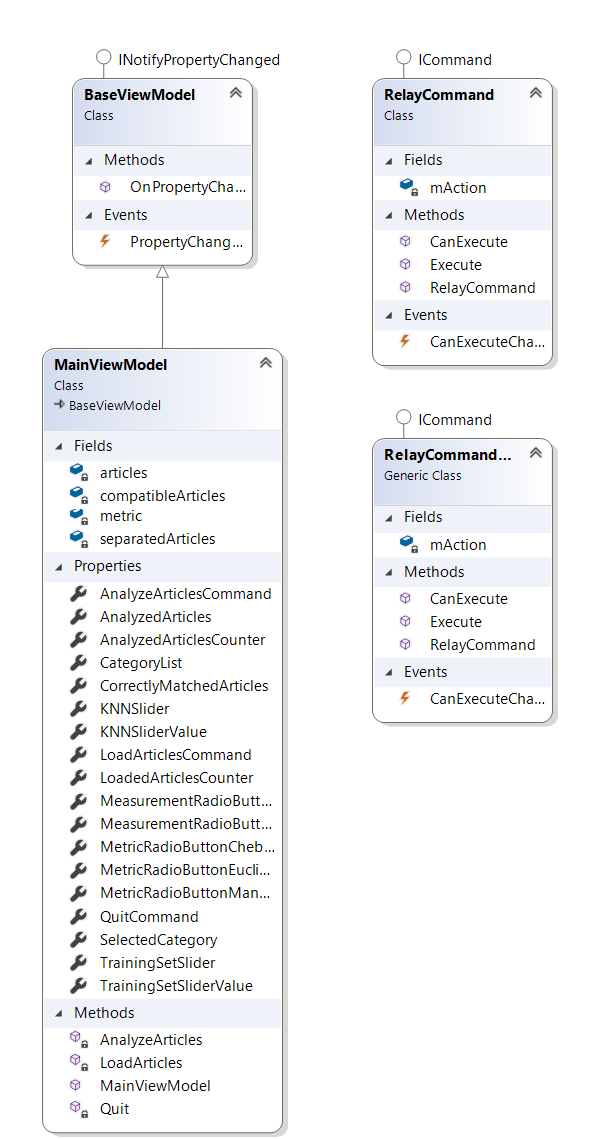
\includegraphics[width=1\textwidth]{{Rysunki/DiagramLogic.png}}
	\caption{Diagram UML wygenerowany dla projektu Logic}
\end{figure}

\subsection{ViewModel}
Projekt ViewModel ma za zadanie odseparować logikę programu od interfejsu graficznego. \newline

Klasa MainViewModel przyjmuje dane wejściowe od użytkownika i reaguje na jego poczynania wywołując wybrane akcje z logiki programu oraz odpowiada za odświeżanie widoków w interfejsie graficznym.

\begin{figure}[H]
	\centering
	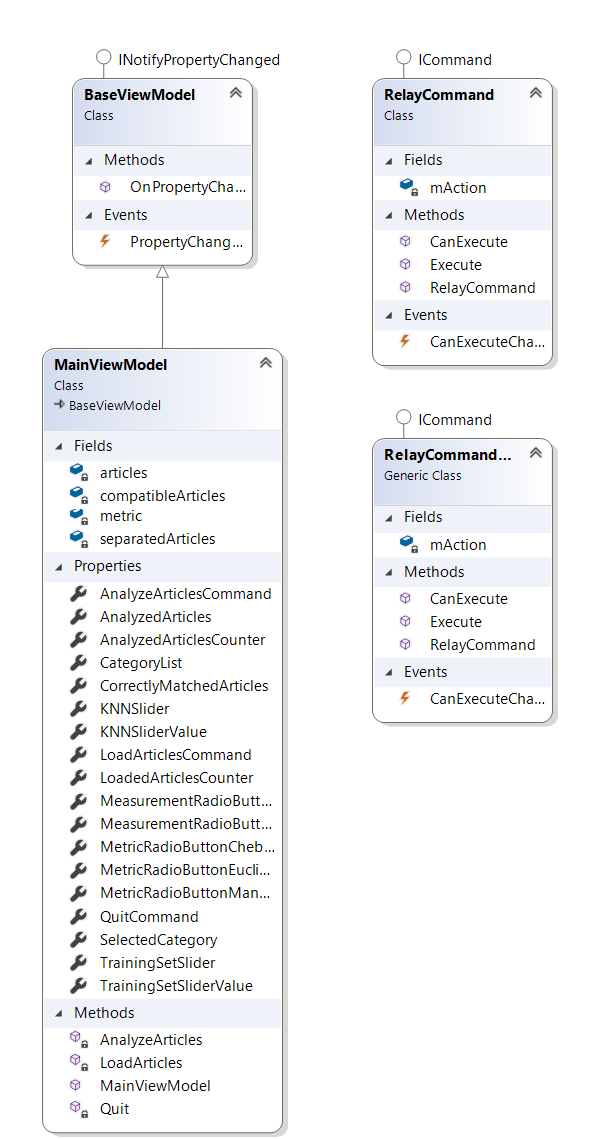
\includegraphics[width=0.9\textwidth]{{Rysunki/DiagramViewModel.png}}
	\caption{Diagram UML wygenerowany dla projektu MainViewModel}
\end{figure}

\subsection{GUI}
Projekt GUI (graphical user interface) implementuje przejrzysty oraz łatwy w obsłudze graficzny interfejs użytkownika. 

\begin{figure}[H]
	\centering
	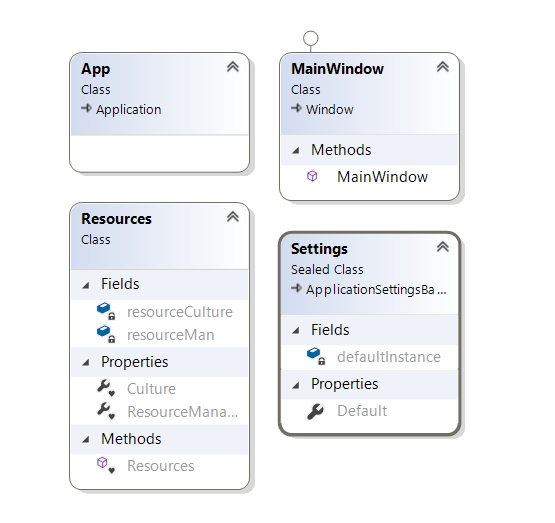
\includegraphics[width=1\textwidth]{{Rysunki/DiagramGUI.png}}
	\caption{Diagram UML wygenerowany dla projektu GUI}
\end{figure}

\section{Materiały i metody}

Klasyfikacja dotycząca lokalizacji przeprowadzana była jedynie na danych, których pole places przyjmowało jedną z wartości: west-germany, usa, france, uk, canada, japan. \newline

Klasyfikacja dotycząca tematów przeprowadzana była jedynie na danych, które pole topics przyjmowało jedną z wartości: gold, cocoa, sugar, coffe, grain. \newline

Danymi jakie sami przygotowaliśmy do analizy były teksty piosenek znanych artystów. Posiadały one jedną kategorię - author. Przyjmowało ono jedną z wartości: taylor swift, macklemore, twenty one pilots, eminem, ed sheeran, black eyed peas.

\subsection{Wpływ liczby k sąsiadów oraz wyboru metryki na klasyfikację}

Klasyfikacja tekstów została wykonana wszystkimi dostępnymi metodami ekstrakcji cech dla wszystkich trzech metryk. Dla każdego przypadku testowego dokonano klasyfikacji tekstu dla k $\in$ \{2, 3, 5, 7, 10, 15, 20\} najbliższych sąsiadów. Zbiór treningowy stanowił zawsze 60\% artykułów, zaś zbiór testowy 40\% artykułów. \newline

\subsection{Wpływ podziału tekstów na zbiory treningowe i testowe na klasyfikację}

Klasyfikacja tekstów została wykonana przy pomocy Term frequency oraz własnych charakterystyk dla metryki Euklidesowej. Dla każdego przypadku testowego dokonano klasyfikacji tekstu dla najodpowiedniejszych k dla danego sposobu ekstrakcji cech oraz metryki. Zbiór treningowy w kolejnych próbach stanowił, 80\% 60\% oraz 40\% artykułów. \newline

\subsection{Wpływ konkretnych cech na klasyfikację}
Klasyfikacja tekstów została wykonana przy pomocy ekstrakcji cech charakterystycznych dla metryki Euklidesowej oraz dla zbioru treningowego stanowiącego 80\% artykułów przy $k = 7$. Badania zostały przeprowadzone na tekstach z tagami topics oraz author. Pierwszy test został przeprowadzony przy wyłączeniu jednej cechy, drugi przy stosowaniu tylko jednej cechy, a trzeci konkretnego zestawu cech. Za każdym razem porównano te wyniki z przypadkiem kiedy wszystkie cechy były włączone.

\section{Wyniki}

Poniższej umieszczone tabele oraz wykresy są wynikami przeprowadzonych przez nas eksperymentów.

\subsection{Wpływ liczby k sąsiadów oraz wyboru metryki na klasyfikację}

\begin{table}[H]
	\centering
	\begin{tabular}{c c c c} 
		\hline
		\textbf{k} & \textbf{places [\%]} & \textbf{topics [\%]} &  \textbf{authors [\%]} \\ [0.5ex] 
		\hline
		\hline 
		2 & 74.4 & 53.7 & 43.9 \\ 
		3 & 78.5 & 52.2 & 43.9 \\
		5 & 80.2 & 52.2 & 36.6 \\
		7 & 81.0 & 53.7 & 26.8 \\
		10 & 81.5 & 60.4 & 24.4 \\
		15 & 81.6 & 62.7 & 29.3 \\
		20 & 81.4 & 61.2 & 31.7 \\ 
		\hline
	\end{tabular}
	\caption{Skuteczność klasyfikacji dla metryki Euklidesowej dla pierwszego sposobu ekstrakcji}
\end{table}

\begin{table}[H]
	\centering
	\begin{tabular}{c c c c} 
		\hline
		\textbf{k} & \textbf{places [\%]} & \textbf{topics [\%]} &  \textbf{authors [\%]} \\ [0.5ex] 
		\hline
		\hline 
		2 & 75.4 & 56.7 & 36.6 \\ 
		3 & 79.4 & 56.7 & 39.0 \\
		5 & 81.0 & 61.2 & 36.6 \\
		7 & 81.3 & 59.0 & 31.7 \\
		10 & 81.9 & 64.9 & 24.4 \\
		15 & 82.0 & 64.9 & 29.3 \\
		20 & 82.1 & 63.4 & 29.3 \\ 
		\hline
	\end{tabular}
	\caption{Skuteczność klasyfikacji dla metryki ulicznej dla pierwszego sposobu ekstrakcji}
\end{table}

\begin{table}[H]
	\centering
	\begin{tabular}{c c c c} 
		\hline
		\textbf{k} & \textbf{places [\%]} & \textbf{topics [\%]} &  \textbf{authors [\%]} \\ [0.5ex] 
		\hline
		\hline 
		2 & 80.3 & 14.9 & 17.1 \\ 
		3 & 80.3 & 44.0 & 17.1 \\
		5 & 80.3 & 44.0 & 17.1 \\
		7 & 80.3 & 44.0 & 17.1 \\
		10 & 80.3 & 44.0 & 17.1 \\
		15 & 80.3 & 44.0 & 17.1 \\
		20 & 80.3 & 44.0 & 17.1 \\ 
		\hline
	\end{tabular}
	\caption{Skuteczność klasyfikacji dla metryki Czebyszewa dla pierwszego sposobu ekstrakcji}
\end{table}

\begin{figure}[H]
	\centering
	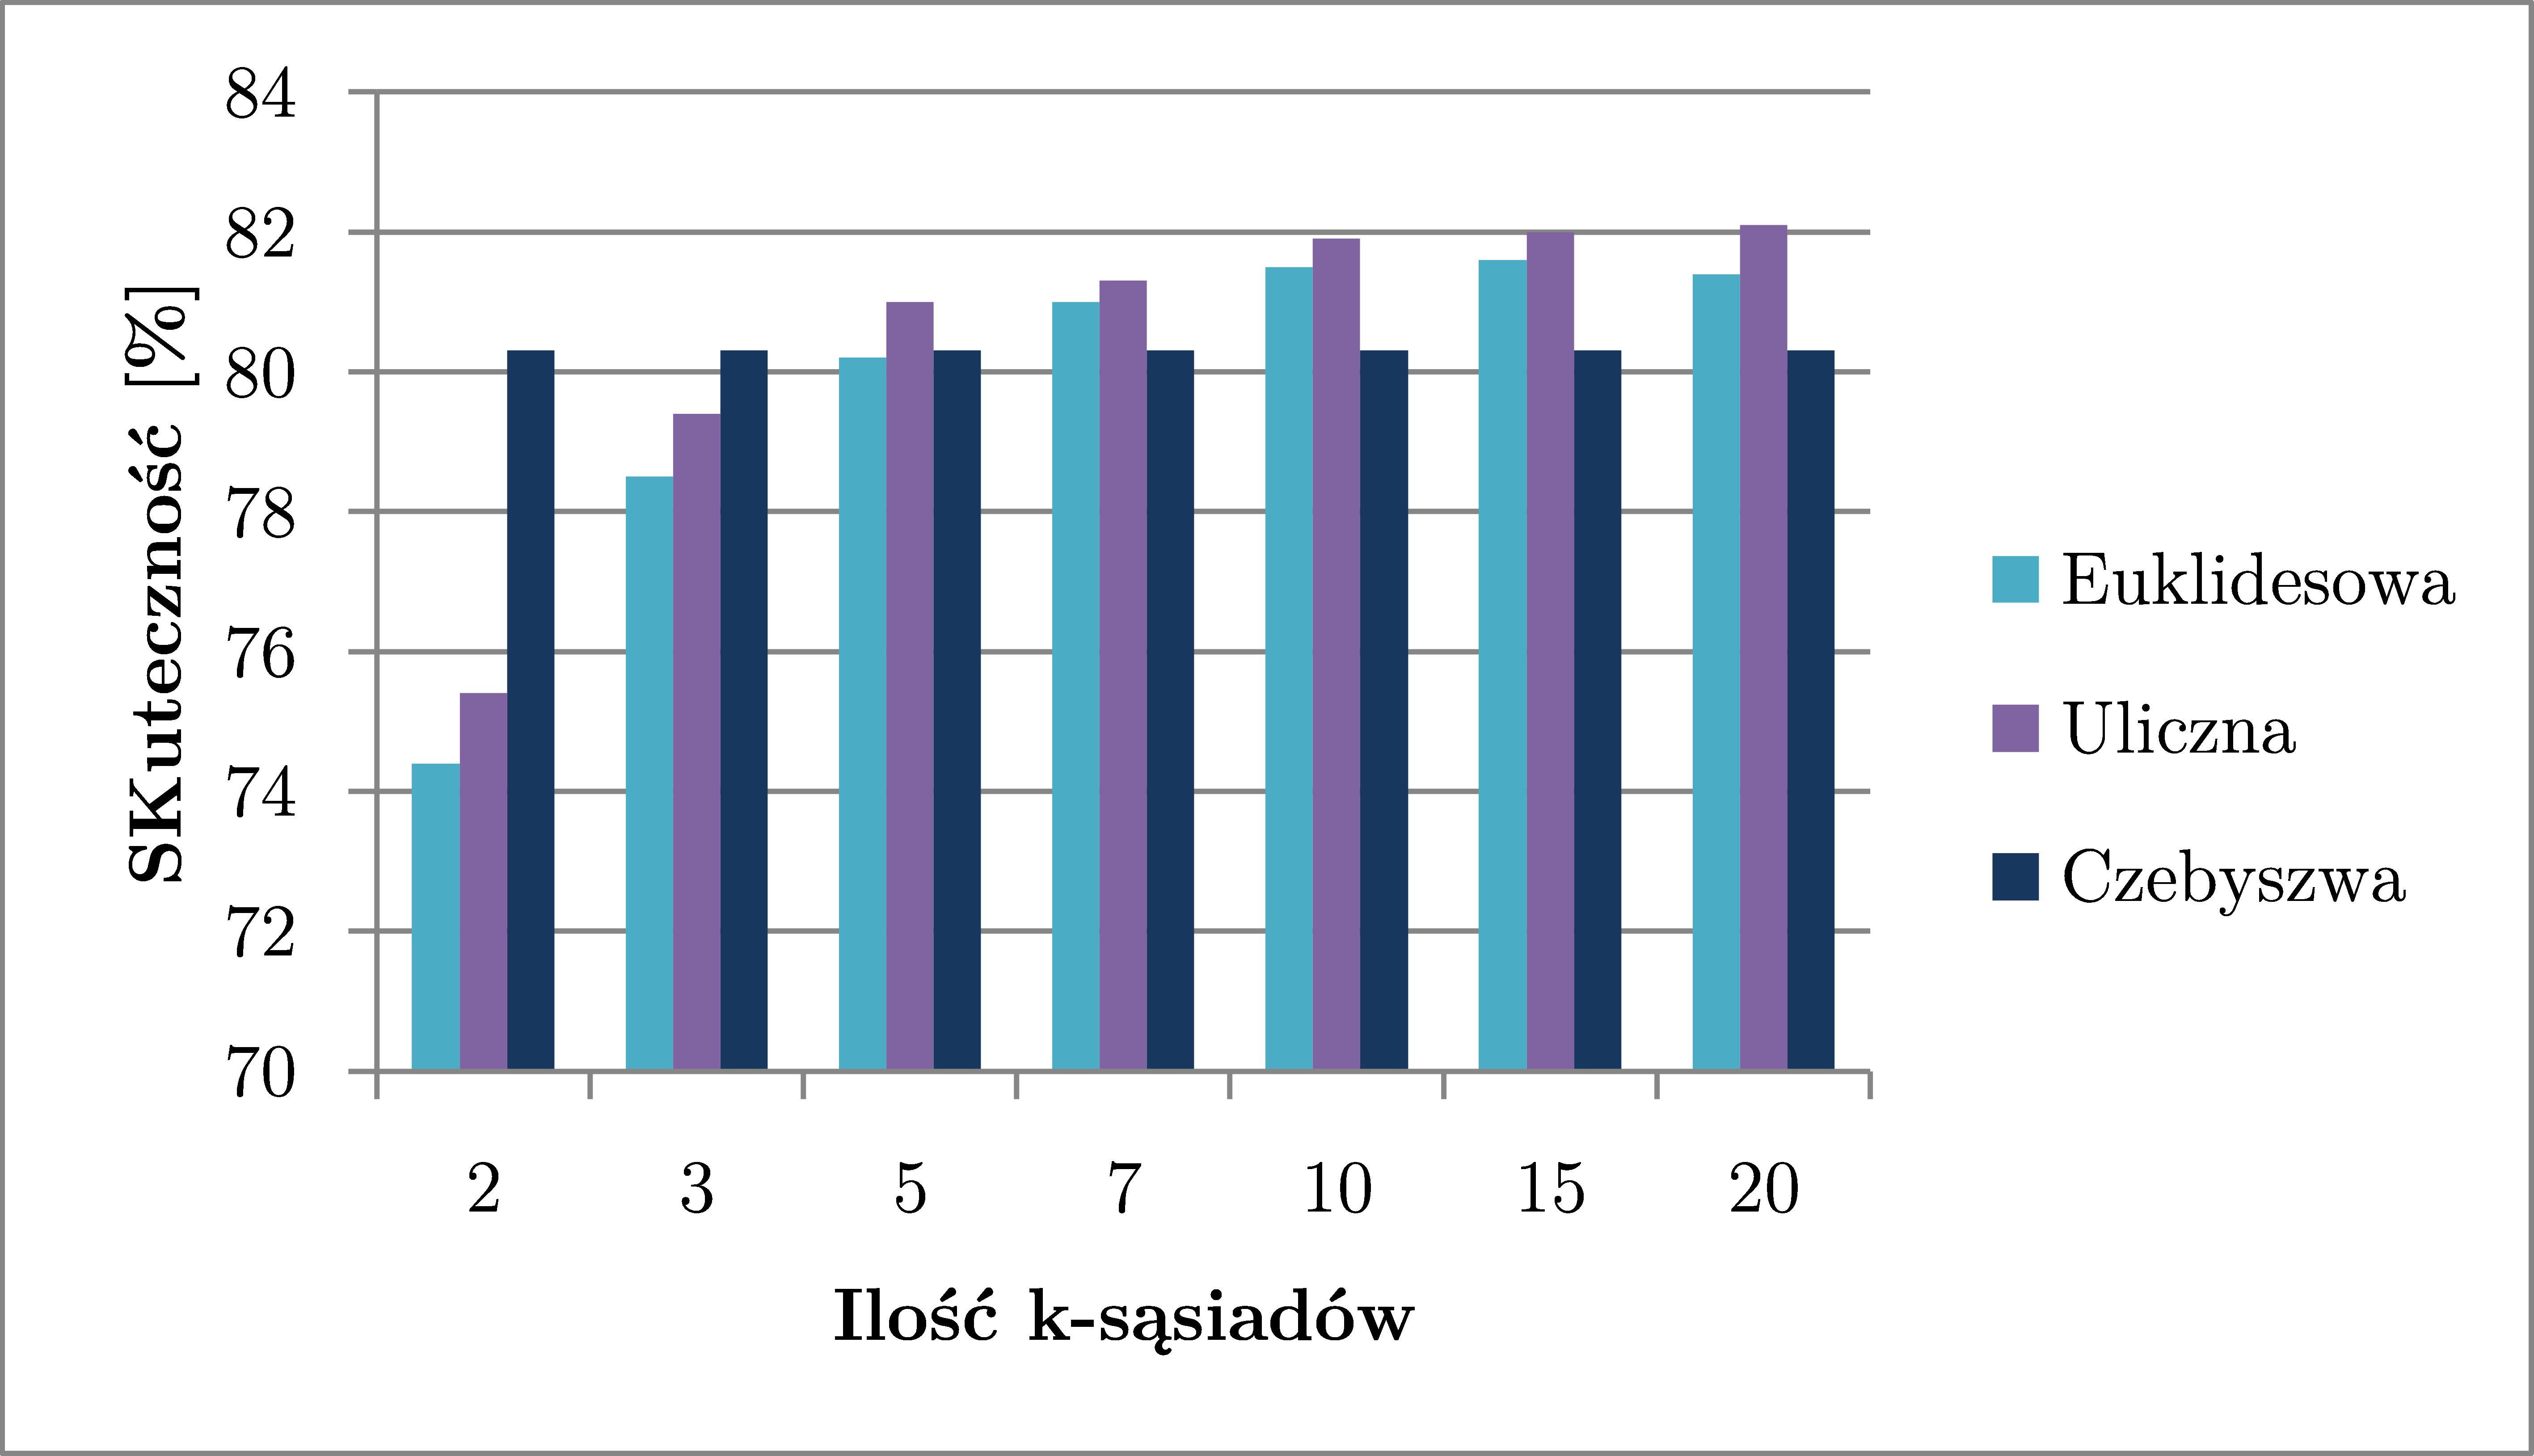
\includegraphics[width=0.9\textwidth]{{Rysunki/TF-places.png}}
	\caption{Dane z Tabel 1-3 dla kategorii places}
\end{figure}

\begin{figure}[H]
	\centering
	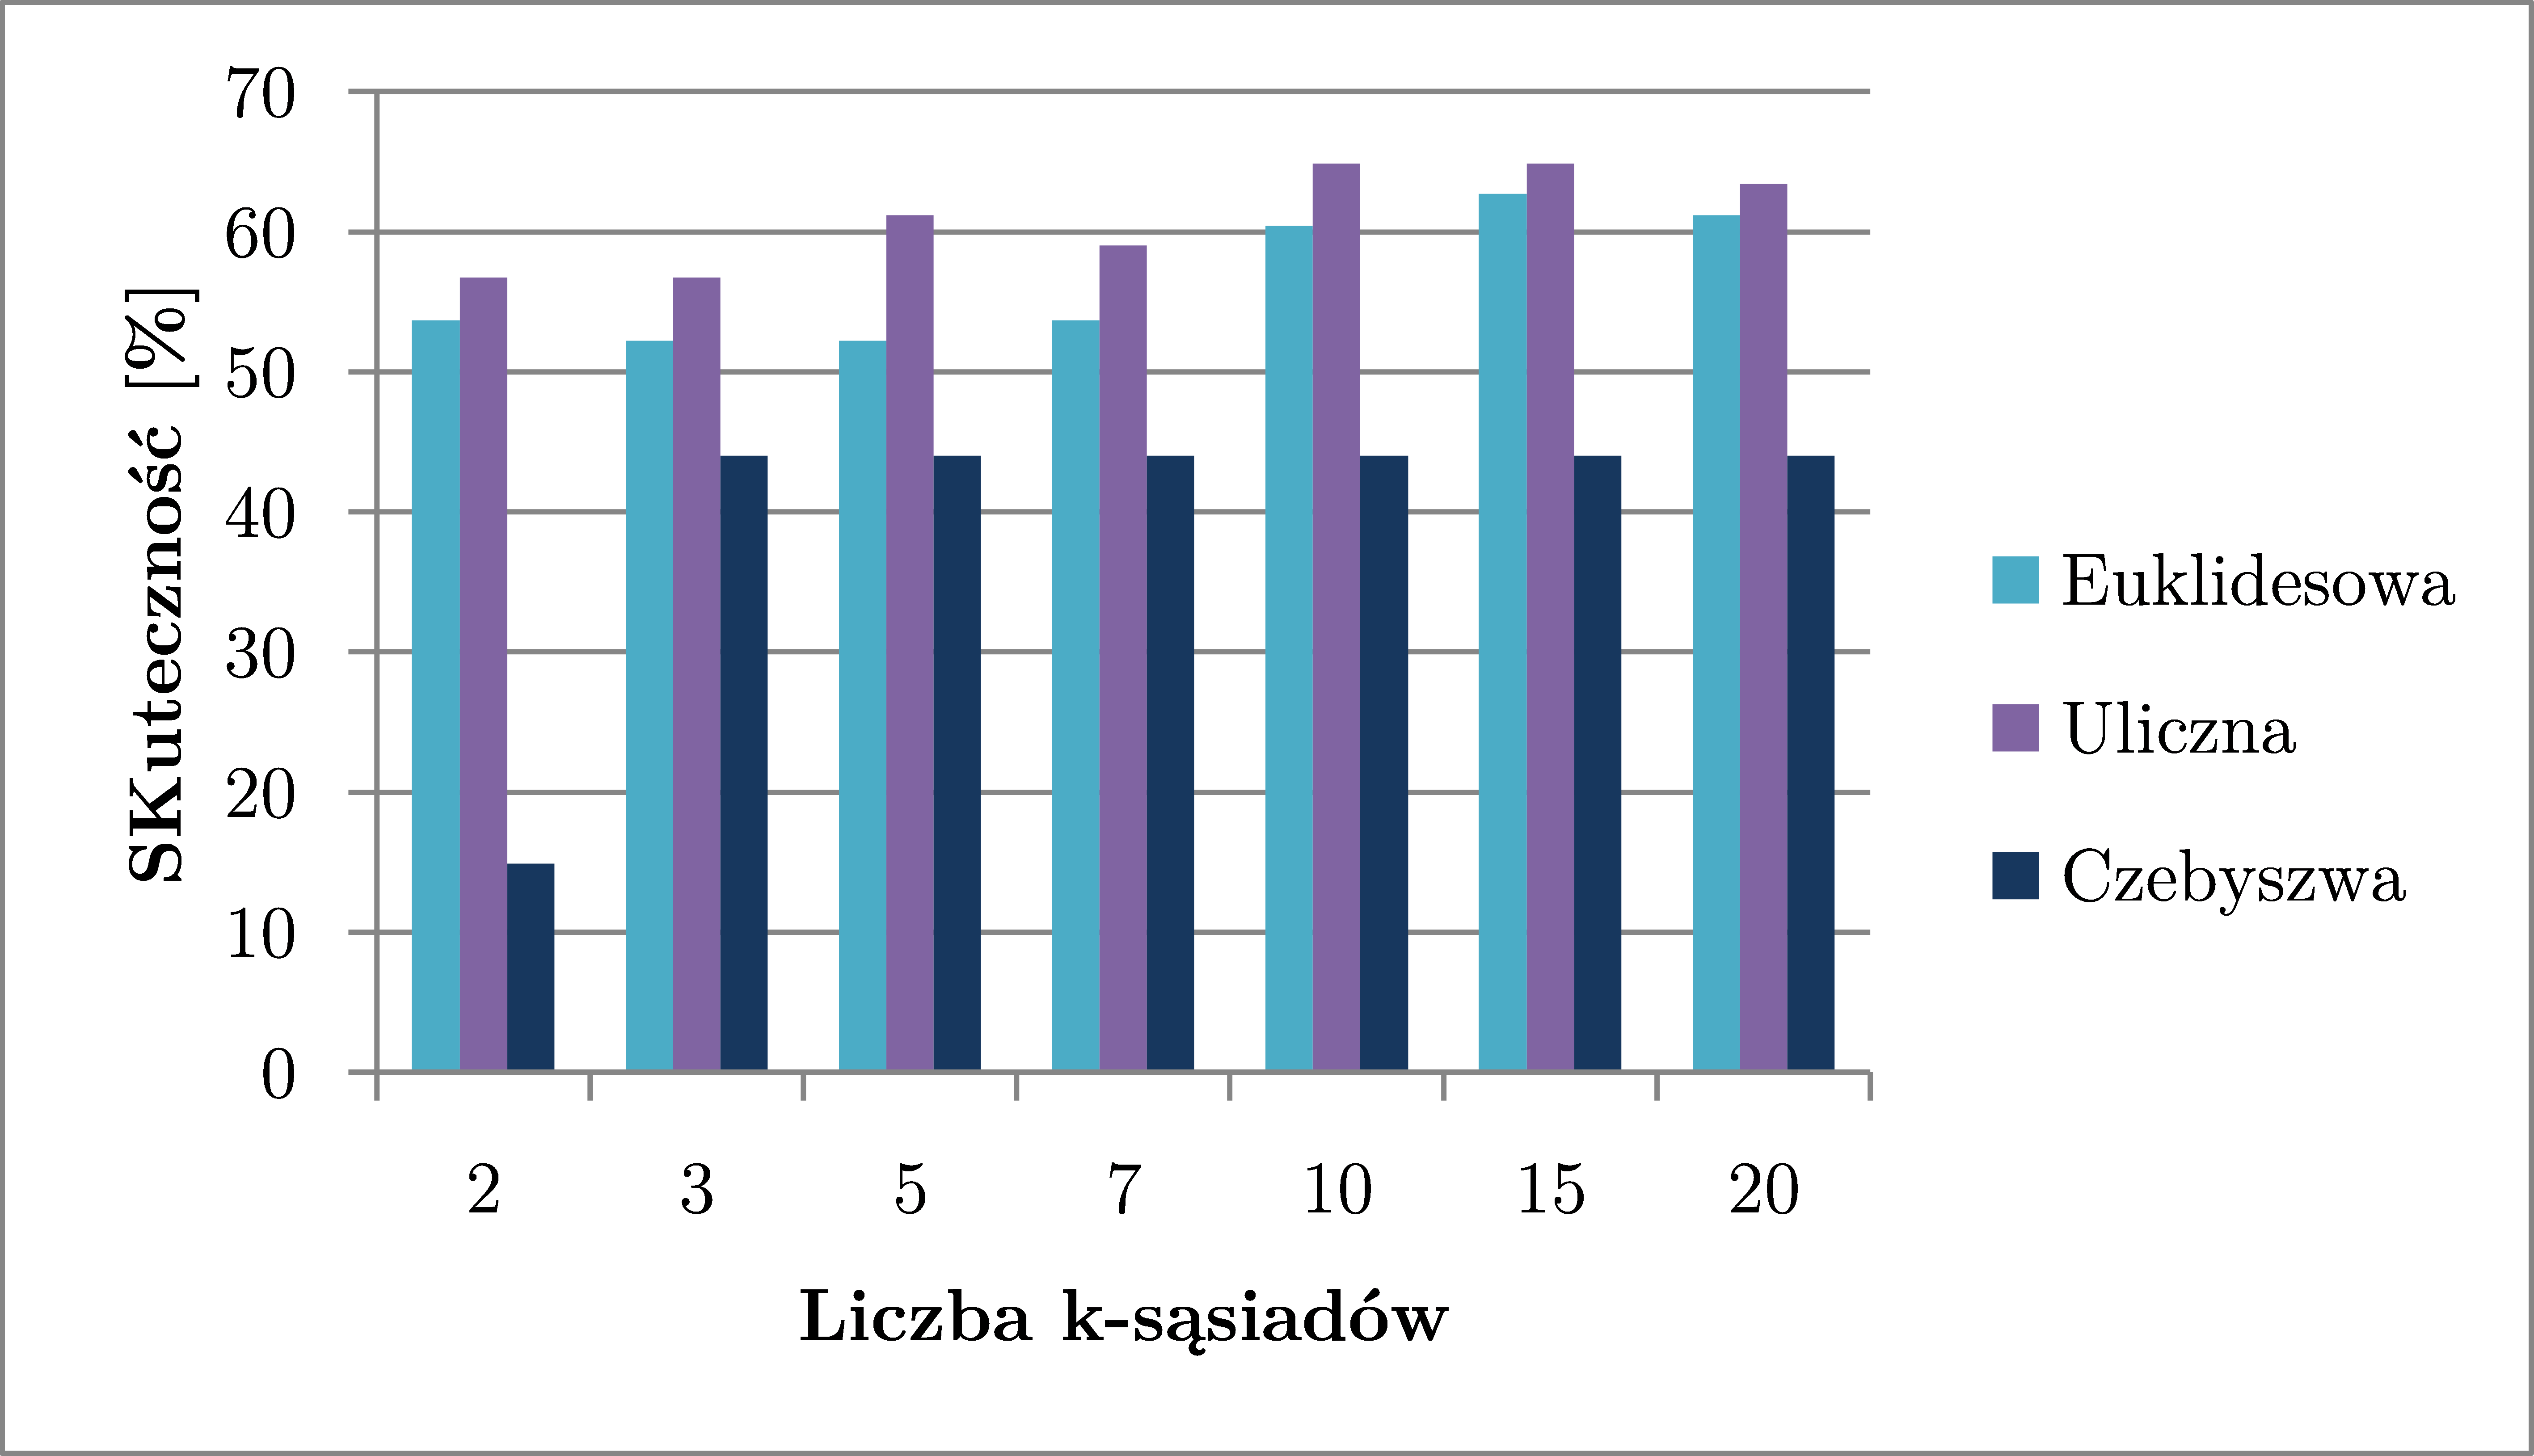
\includegraphics[width=0.9\textwidth]{{Rysunki/TF-topics.png}}
	\caption{Dane z Tabel 1-3 dla kategorii topics}
\end{figure}

\begin{figure}[H]
	\centering
	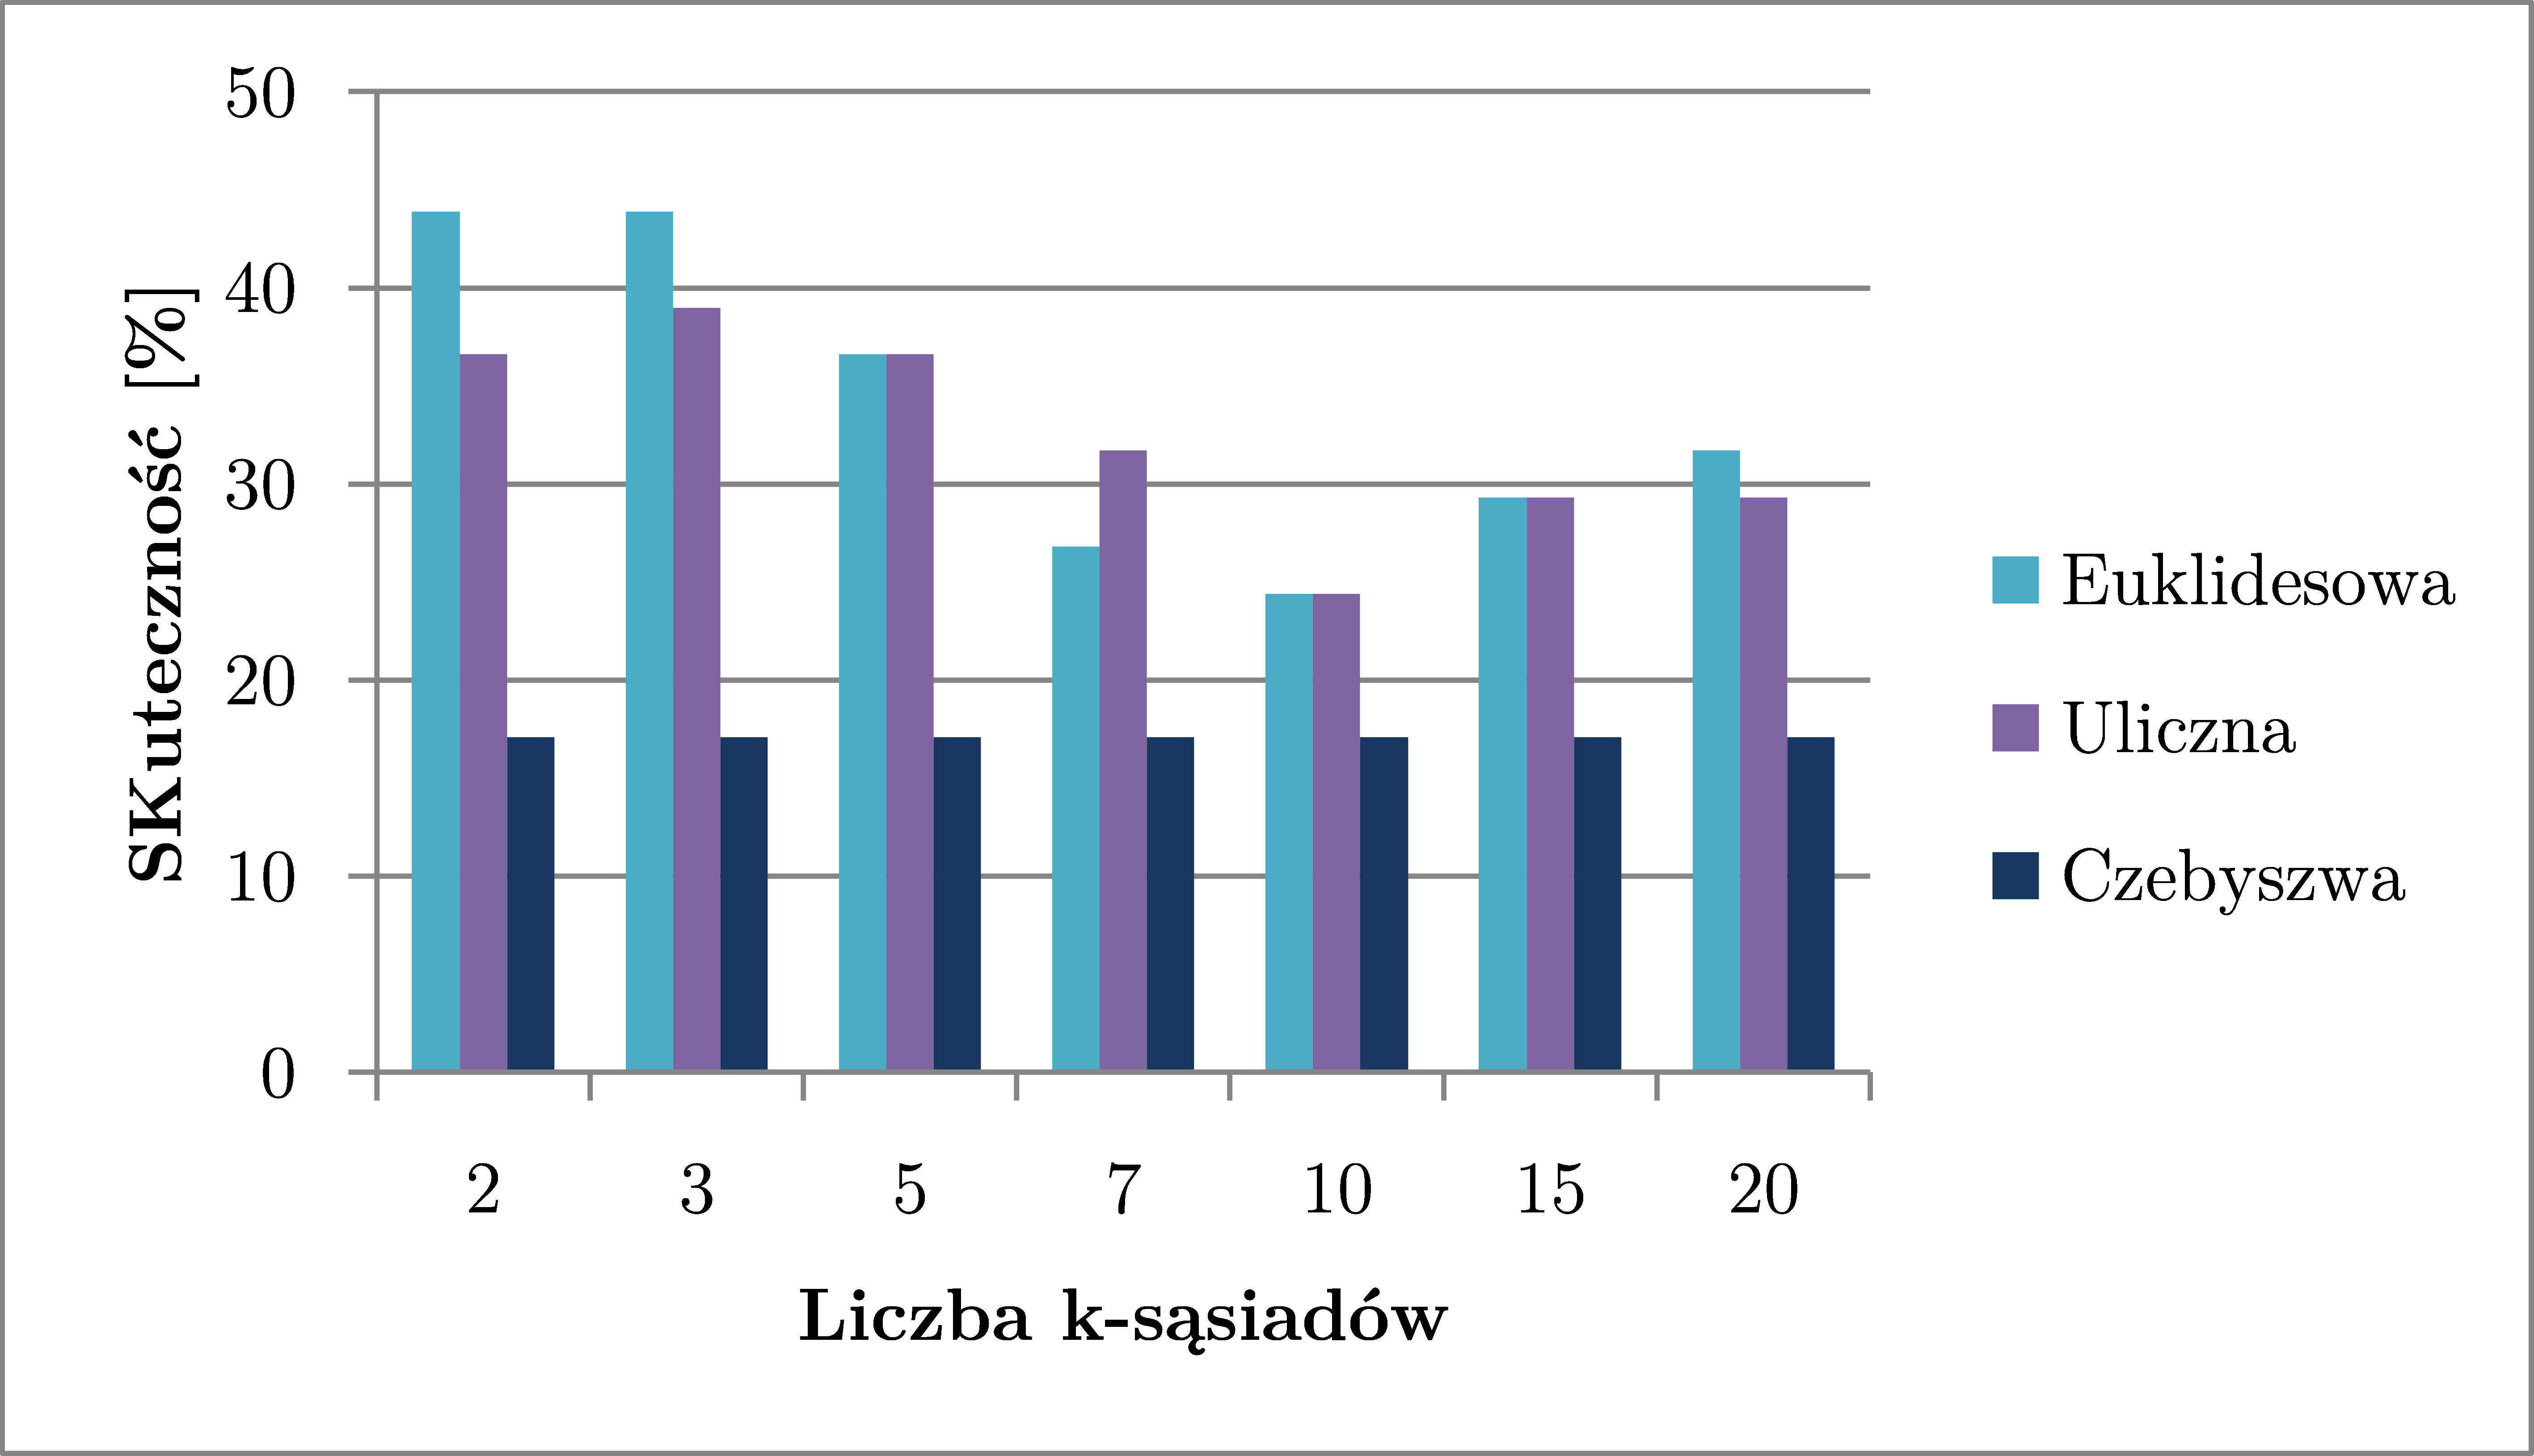
\includegraphics[width=0.9\textwidth]{{Rysunki/TF-authors.png}}
	\caption{Dane z Tabel 1-3 dla kategorii authors (własne teksty)}
\end{figure}

\begin{table}[H]
	\centering
	\begin{tabular}{c c c c} 
		\hline
		\textbf{k} & \textbf{places [\%]} & \textbf{topics [\%]} &  \textbf{authors [\%]} \\ [0.5ex] 
		\hline
		\hline 
		2 & 79.0 & 63.4 & 22.0 \\ 
		3 & 82.0 & 64.2 & 19.5 \\
		5 & 82.1 & 59.0 & 29.3 \\
		7 & 83.3 & 62.1 & 22.0 \\
		10 & 82.0 & 64.9 & 26.8 \\
		15 & 81.9 & 67.9 & 24.4 \\
		20 & 81.1 & 67.1 & 17.1 \\ 
		\hline
	\end{tabular}
	\caption{Skuteczność klasyfikacji dla metryki Euklidesowej dla drugiego sposobu ekstrakcji}
\end{table}

\begin{table}[H]
	\centering
	\begin{tabular}{c c c c} 
		\hline
		\textbf{k} & \textbf{places [\%]} & \textbf{topics [\%]} &  \textbf{authors [\%]} \\ [0.5ex] 
		\hline
		\hline 
		2 & 80.2 & 59.7 & 22.0 \\ 
		3 & 82.4 & 65.7 & 19.5 \\
		5 & 82.6 & 67.2 & 29.3 \\
		7 & 83.3 & 67.2 & 22.0 \\
		10 & 82.6 & 67.2 & 26.8 \\
		15 & 82.1 & 67.2 & 24.4 \\
		20 & 81.6 & 67.9 & 17.1 \\ 
		\hline
	\end{tabular}
	\caption{Skuteczność klasyfikacji dla metryki ulicznej dla drugiego sposobu ekstrakcji}
\end{table}

\begin{table}[H]
	\centering
	\begin{tabular}{c c c c} 
		\hline
		\textbf{k} & \textbf{places [\%]} & \textbf{topics [\%]} &  \textbf{authors [\%]} \\ [0.5ex] 
		\hline
		\hline 
		2 & 77.0 & 14.9 & 17.1 \\ 
		3 & 77.0 & 44.0 & 17.1 \\
		5 & 77.0 & 44.0 & 17.1 \\
		7 & 77.0 & 44.0 & 17.1 \\
		10 & 77.0 & 44.0 & 17.1 \\
		15 & 77.0 & 44.0 & 17.1 \\
		20 & 77.0 & 44.0 & 17.1 \\ 
		\hline
	\end{tabular}
	\caption{Skuteczność klasyfikacji dla metryki Czebyszewa dla drugiego sposobu ekstrakcji}
\end{table}

\begin{figure}[H]
	\centering
	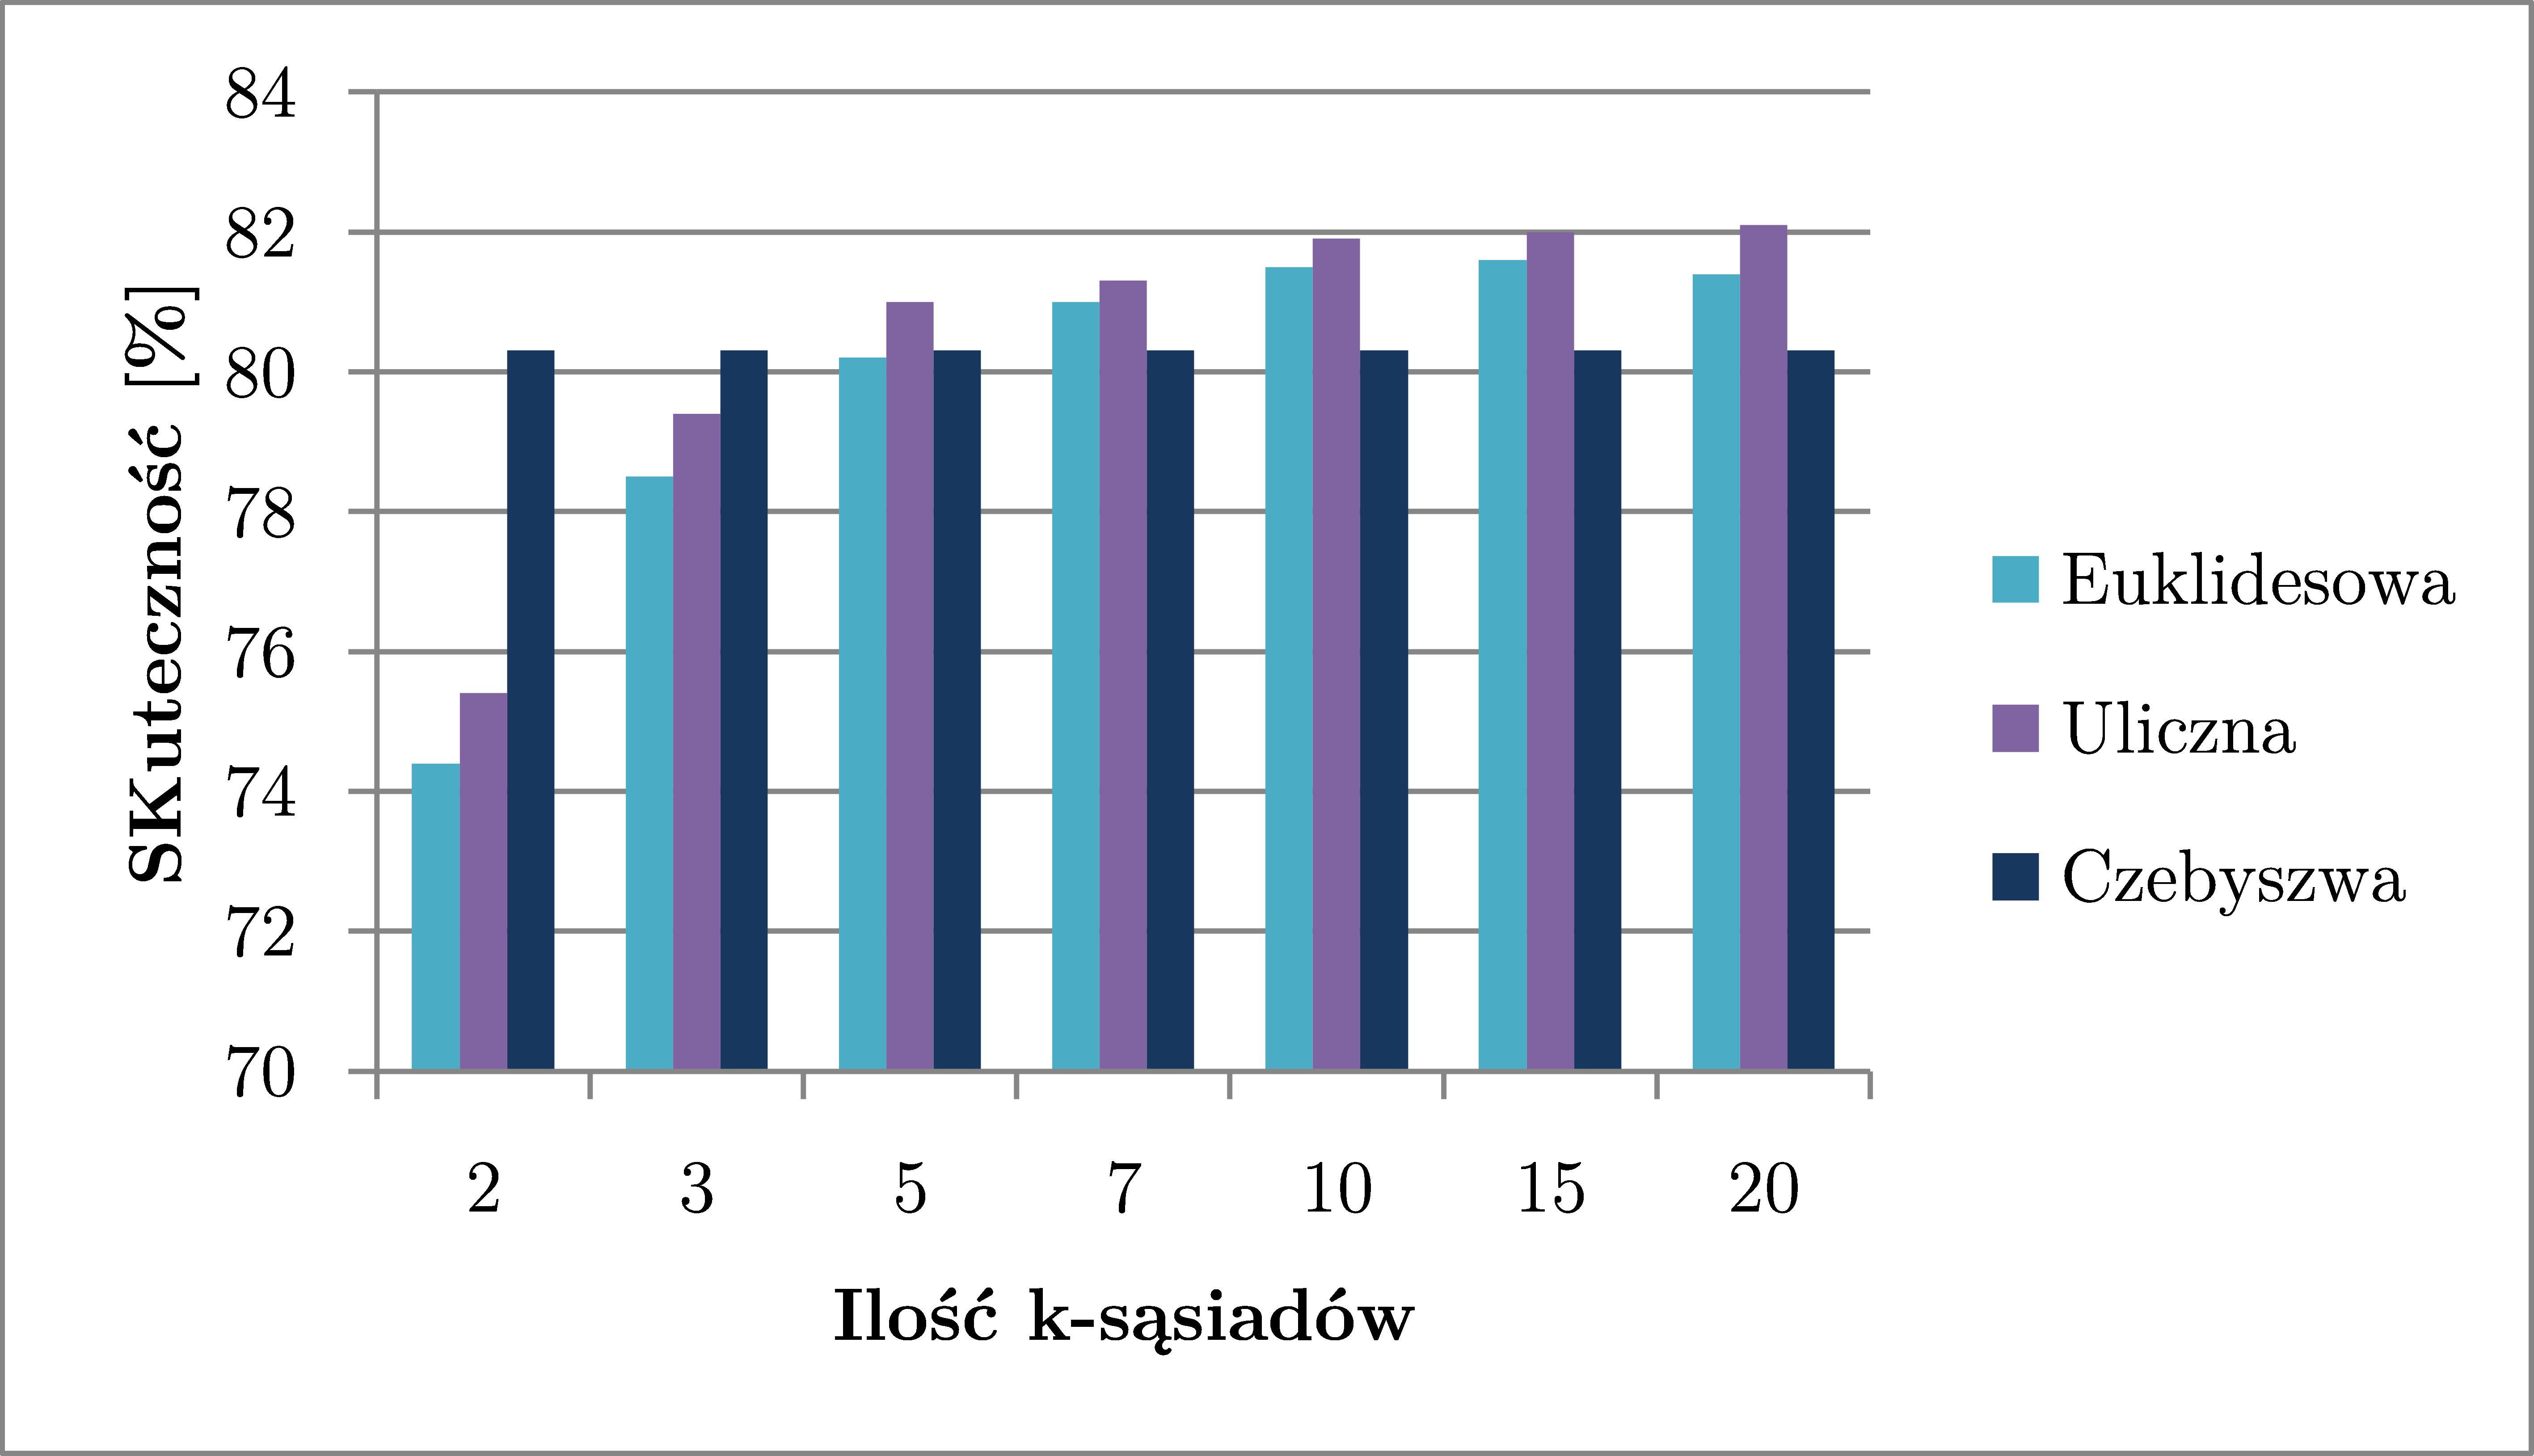
\includegraphics[width=0.9\textwidth]{{Rysunki/TF-places.png}}
	\caption{Dane z Tabel 4-6 dla kategorii places}
\end{figure}

\begin{figure}[H]
	\centering
	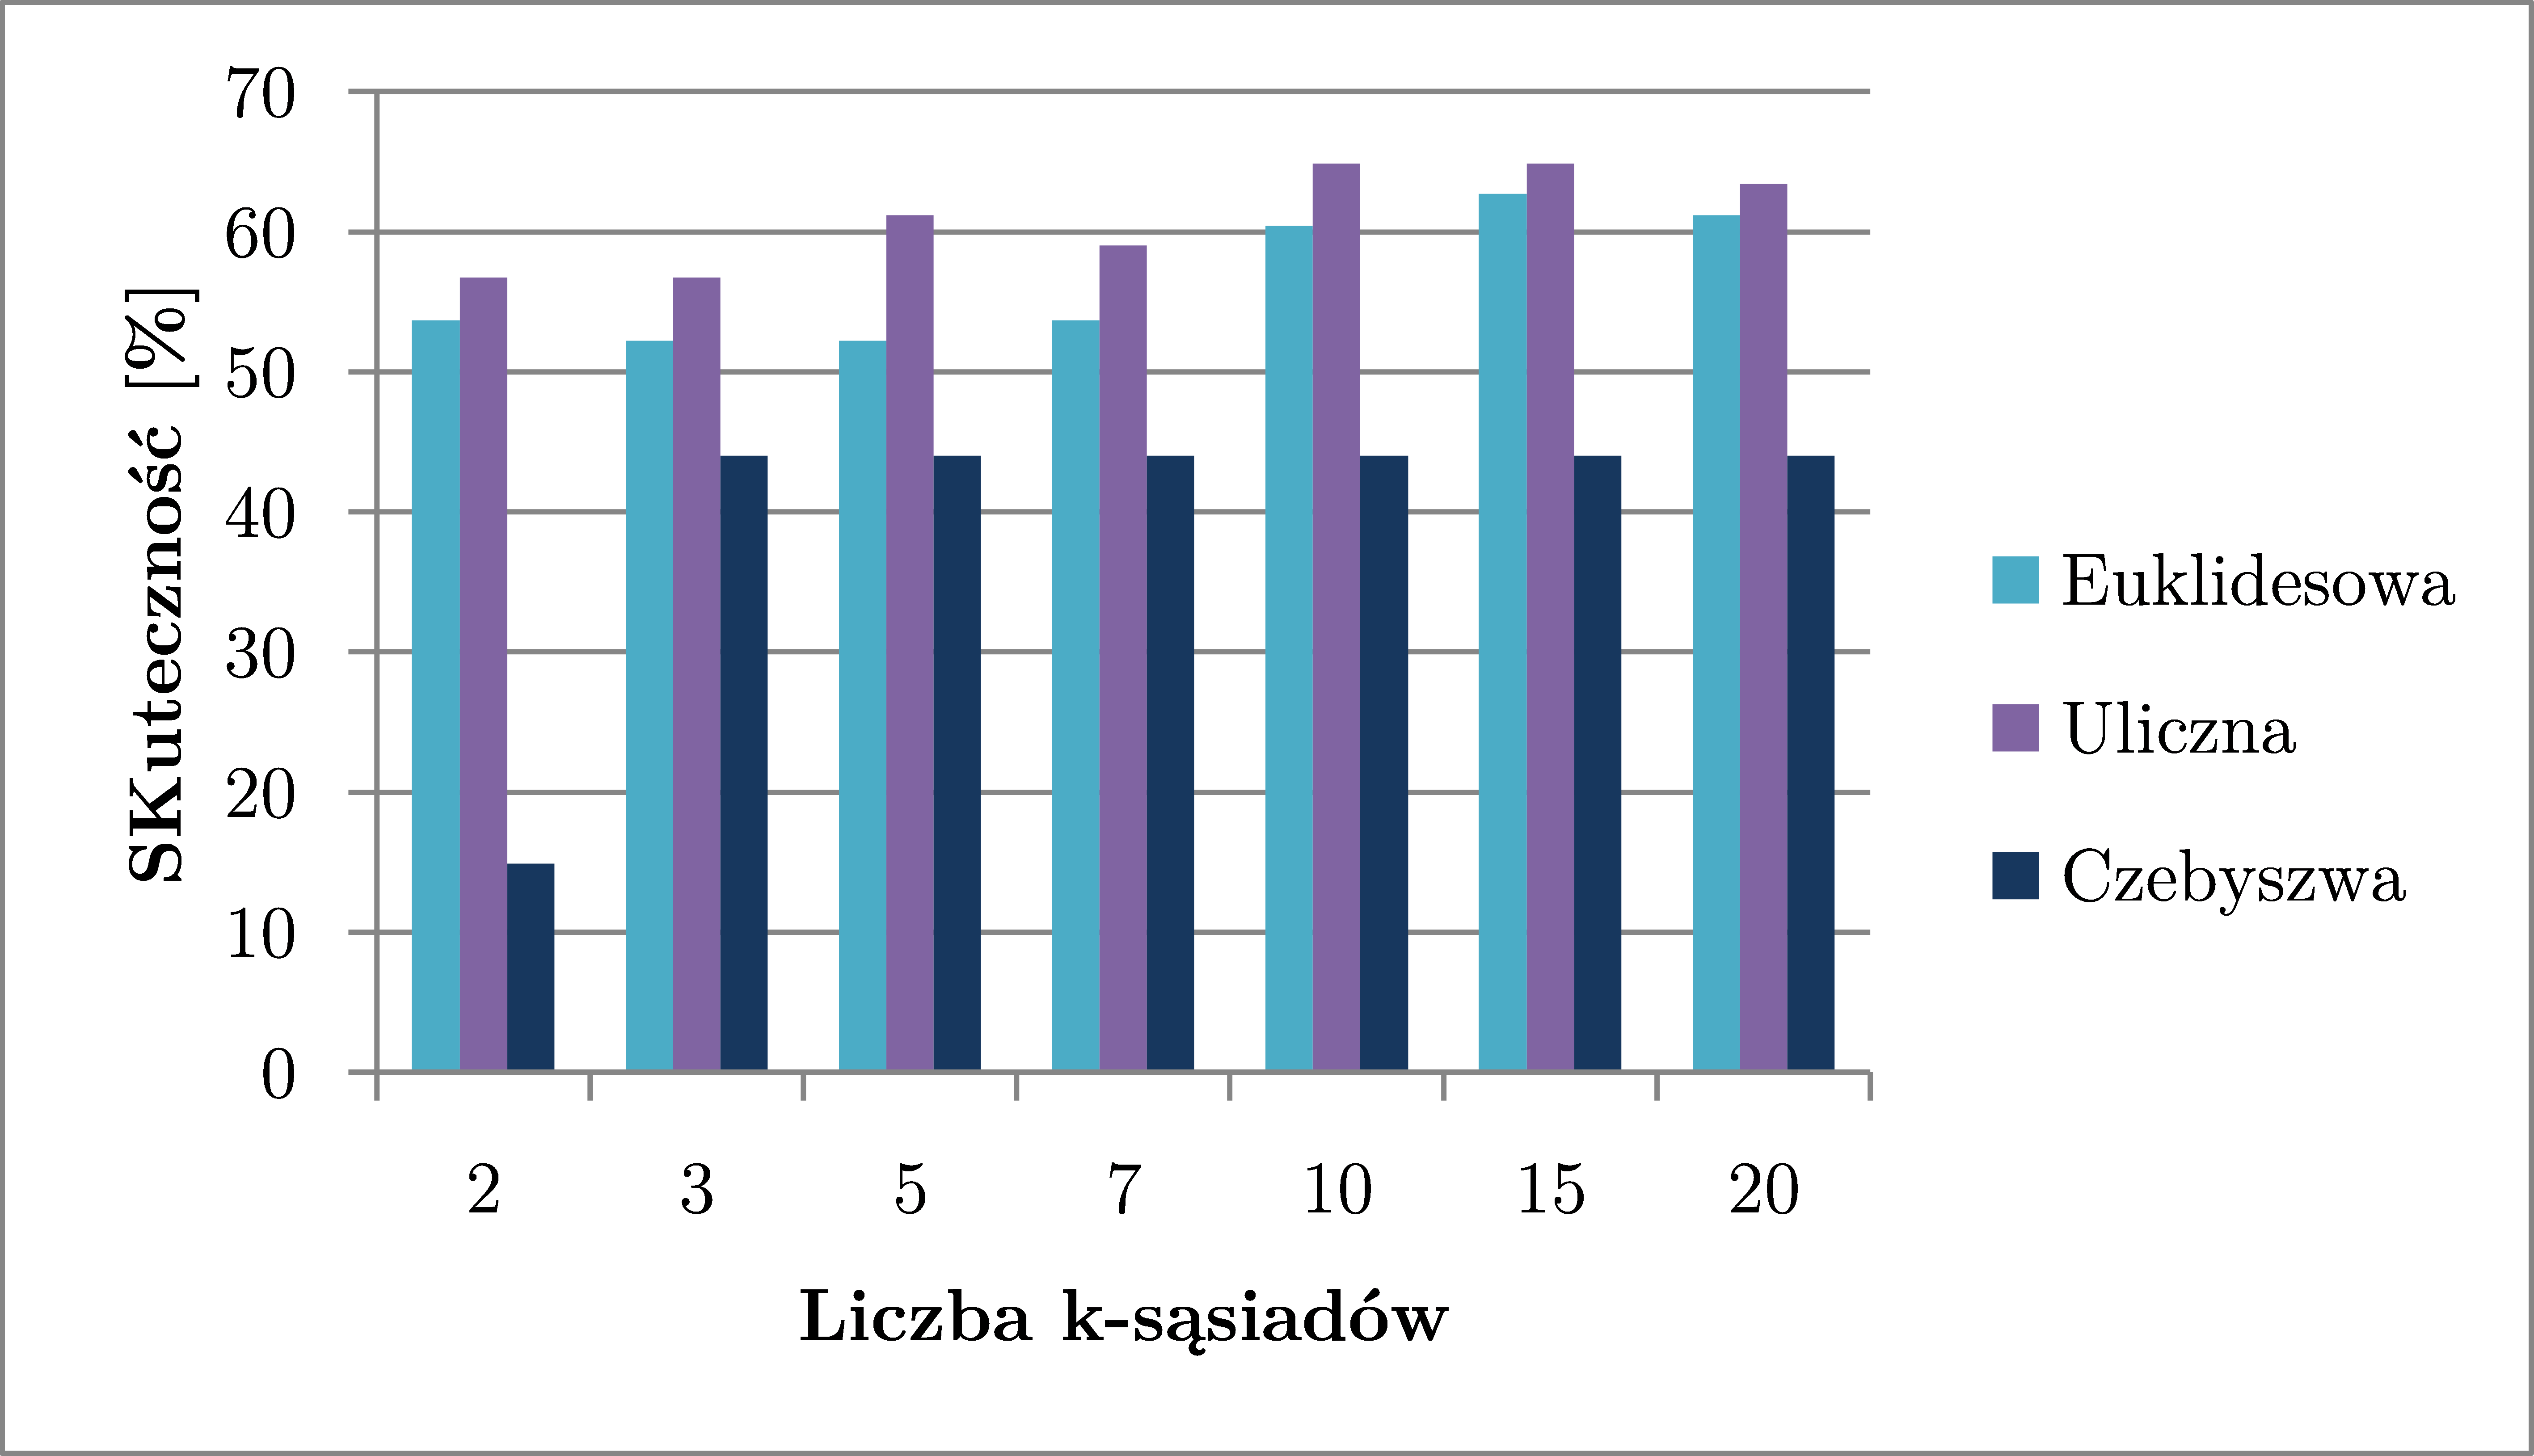
\includegraphics[width=0.9\textwidth]{{Rysunki/TF-topics.png}}
	\caption{Dane z Tabel 4-6 dla kategorii topics}
\end{figure}

\begin{figure}[H]
	\centering
	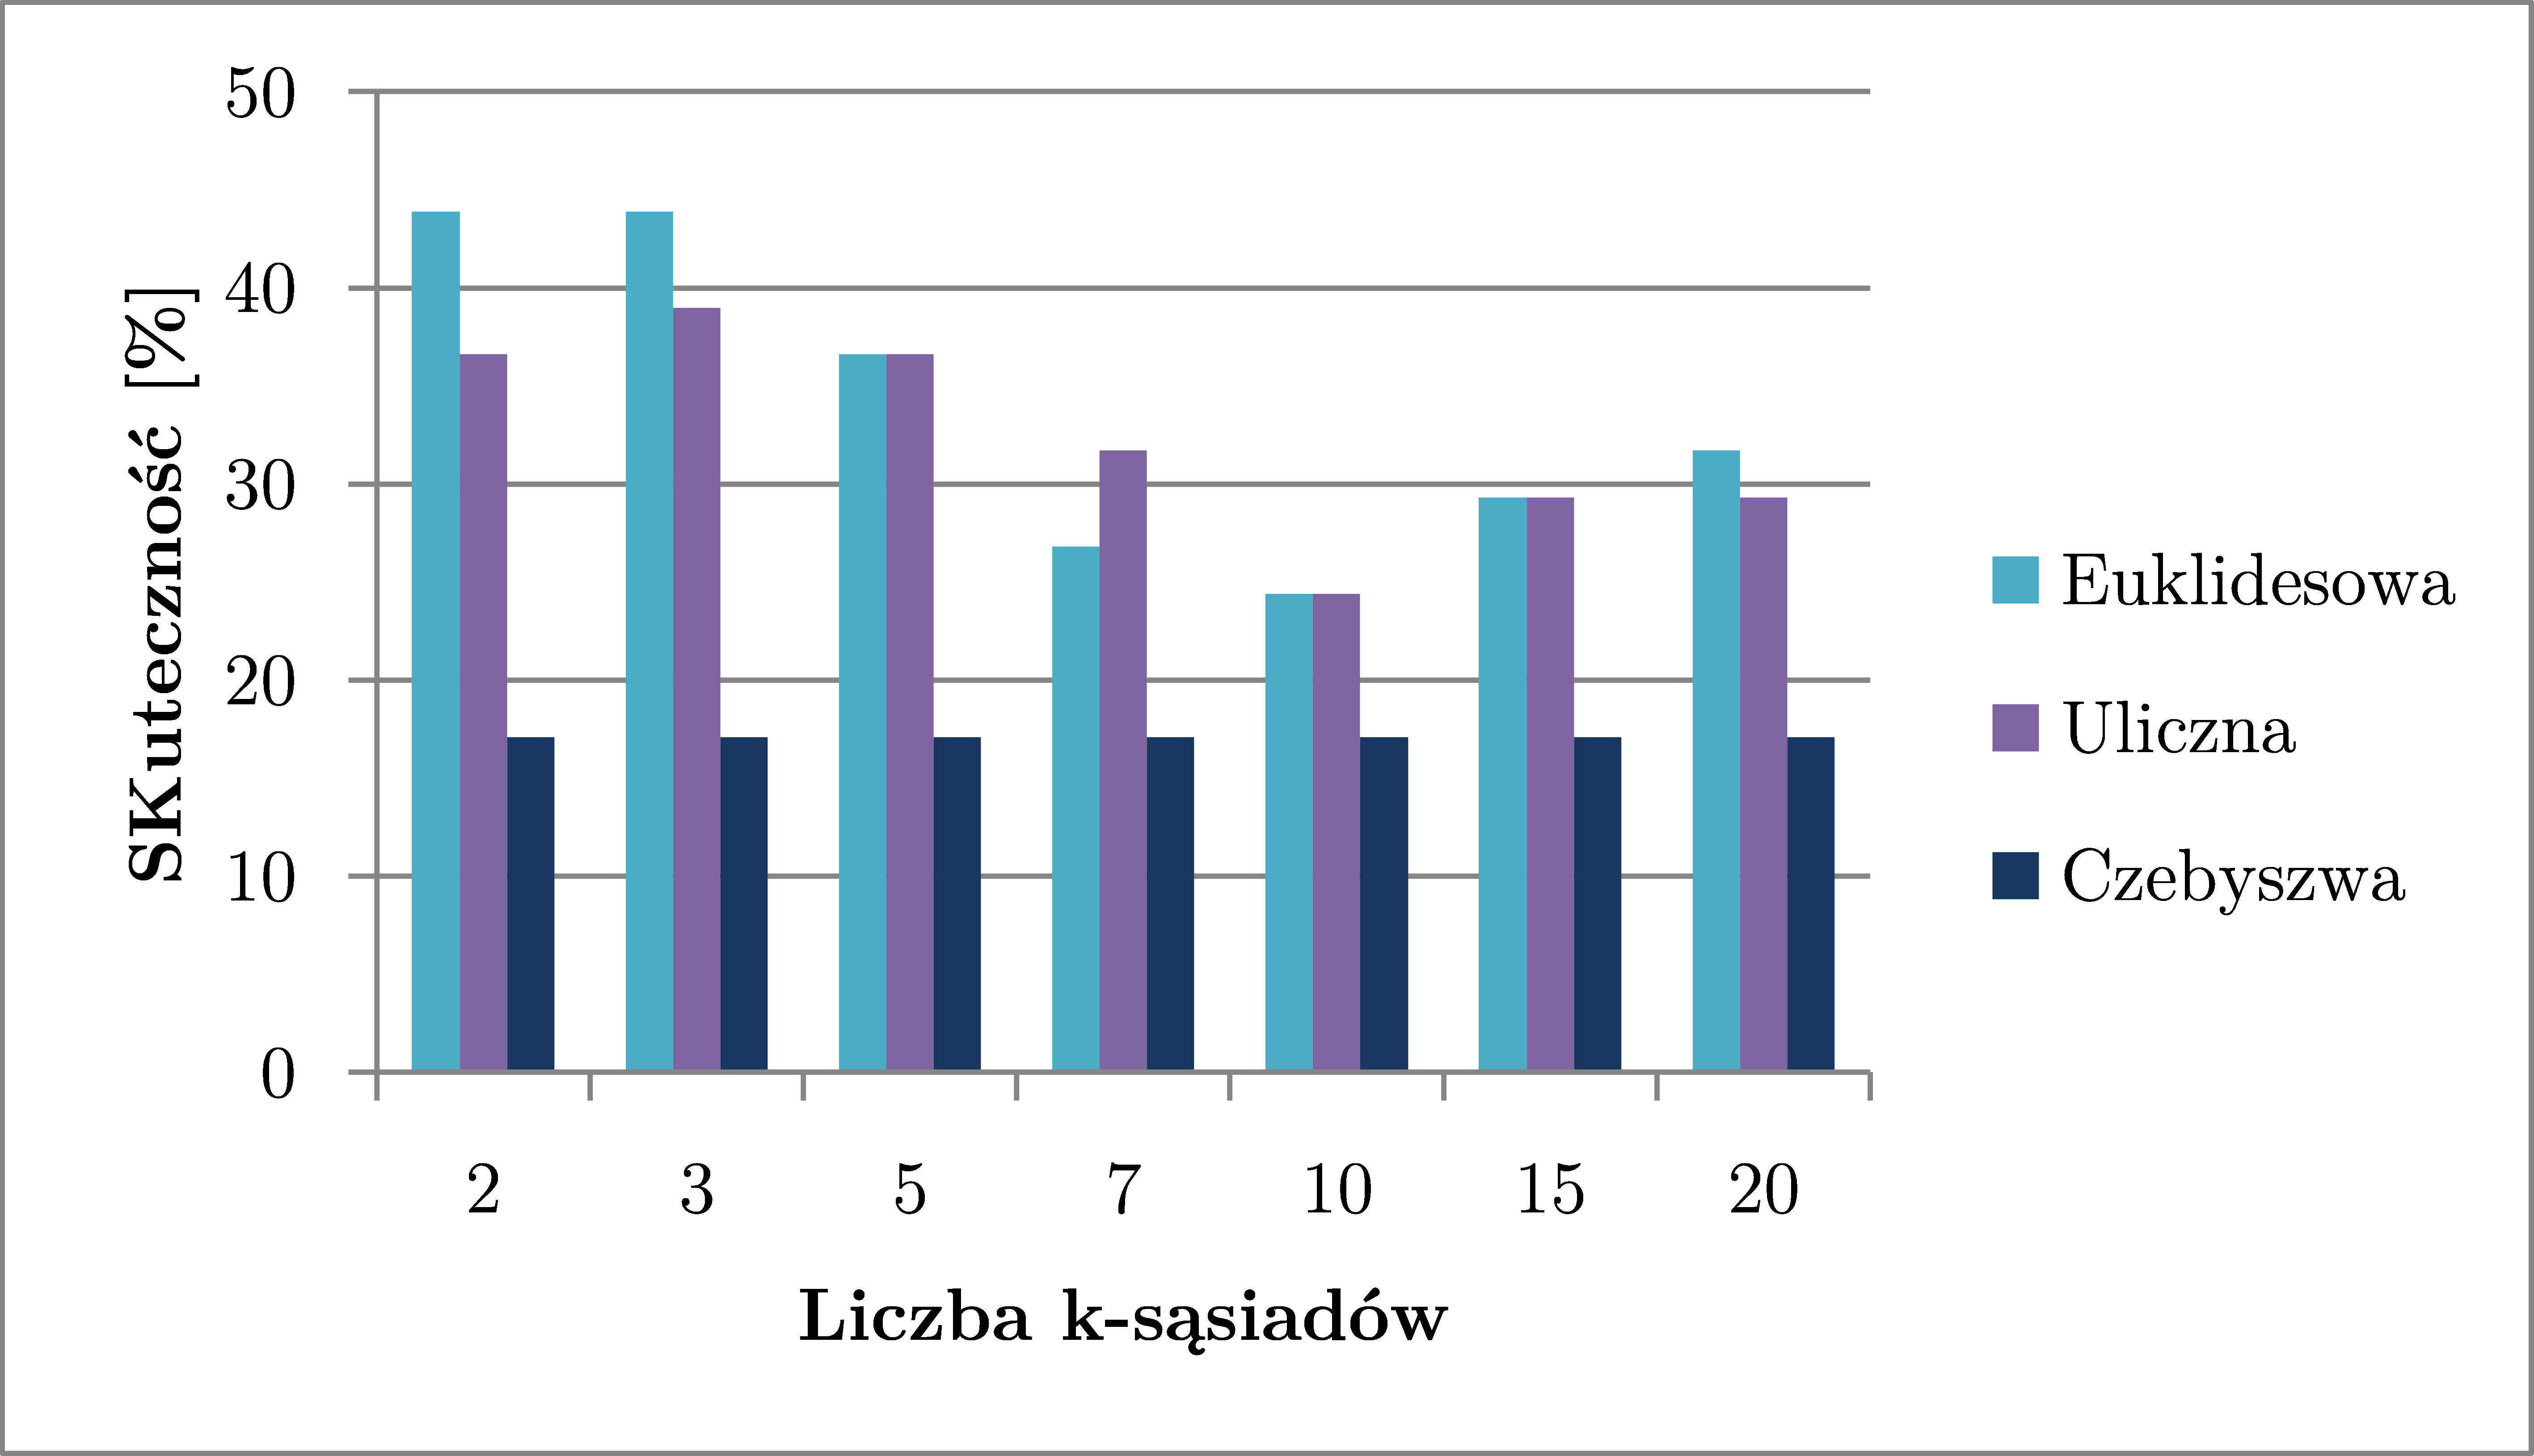
\includegraphics[width=0.9\textwidth]{{Rysunki/TF-authors.png}}
	\caption{Dane z Tabel 4-6 dla kategorii authors (własne teksty)}
\end{figure}

\begin{table}[H]
	\centering
	\begin{tabular}{c c c c} 
		\hline
		\textbf{k} & \textbf{places [\%]} & \textbf{topics [\%]} &  \textbf{authors [\%]} \\ [0.5ex] 
		\hline
		\hline 
		2 & 69.5 & 47.8 & 44.8 \\ 
		3 & 75.3 & 53 & 53.7 \\
		5 & 78.3 & 47 & 48.8 \\
		7 & 79.4 & 48.5 & 63.4 \\
		10 & 80.2 & 49.3 & 63.4 \\
		15 & 80.5 & 47.8 & 58.5 \\
		20 & 80.7 & 44.8 & 53.7 \\ 
		\hline
	\end{tabular}
	\caption{Skuteczność klasyfikacji dla metryki Euklidesowej dla trzeciego sposobu ekstrakcji}
\end{table}

\begin{table}[H]
	\centering
	\begin{tabular}{c c c c} 
		\hline
		\textbf{k} & \textbf{places [\%]} & \textbf{topics [\%]} &  \textbf{authors [\%]} \\ [0.5ex] 
		\hline
		\hline 
		2 & 69 & 49.3 & 56.1 \\ 
		3 & 75.1 & 47 & 56.1 \\
		5 & 78.2 & 47 & 48.8 \\
		7 & 79.3 & 46.3 & 58.5 \\
		10 & 80 & 51.5 & 61 \\
		15 & 80.5 & 45.5 & 58.5 \\
		20 & 80.7 & 45.5 & 56.1 \\ 
		\hline
	\end{tabular}
	\caption{Skuteczność klasyfikacji dla metryki ulicznej dla trzeciego sposobu ekstrakcji}
\end{table}

\begin{table}[H]
	\centering
	\begin{tabular}{c c c c} 
		\hline
		\textbf{k} & \textbf{places [\%]} & \textbf{topics [\%]} &  \textbf{authors [\%]} \\ [0.5ex] 
		\hline
		\hline 
		2 & 80.3 & 14.9 & 17.1 \\ 
		3 & 80.4 & 44 & 17.1 \\
		5 & 80.5 & 44 & 17.1 \\
		7 & 80.6 & 44 & 17.1 \\
		10 & 80.7 & 44 & 17.1 \\
		15 & 80.8 & 44 & 17.1 \\
		20 & 80.9 & 44 & 17.1 \\ 
		\hline
	\end{tabular}
	\caption{Skuteczność klasyfikacji dla metryki Czebyszewa dla trzeciego sposobu ekstrakcji}
\end{table}

\begin{figure}[H]
	\centering
	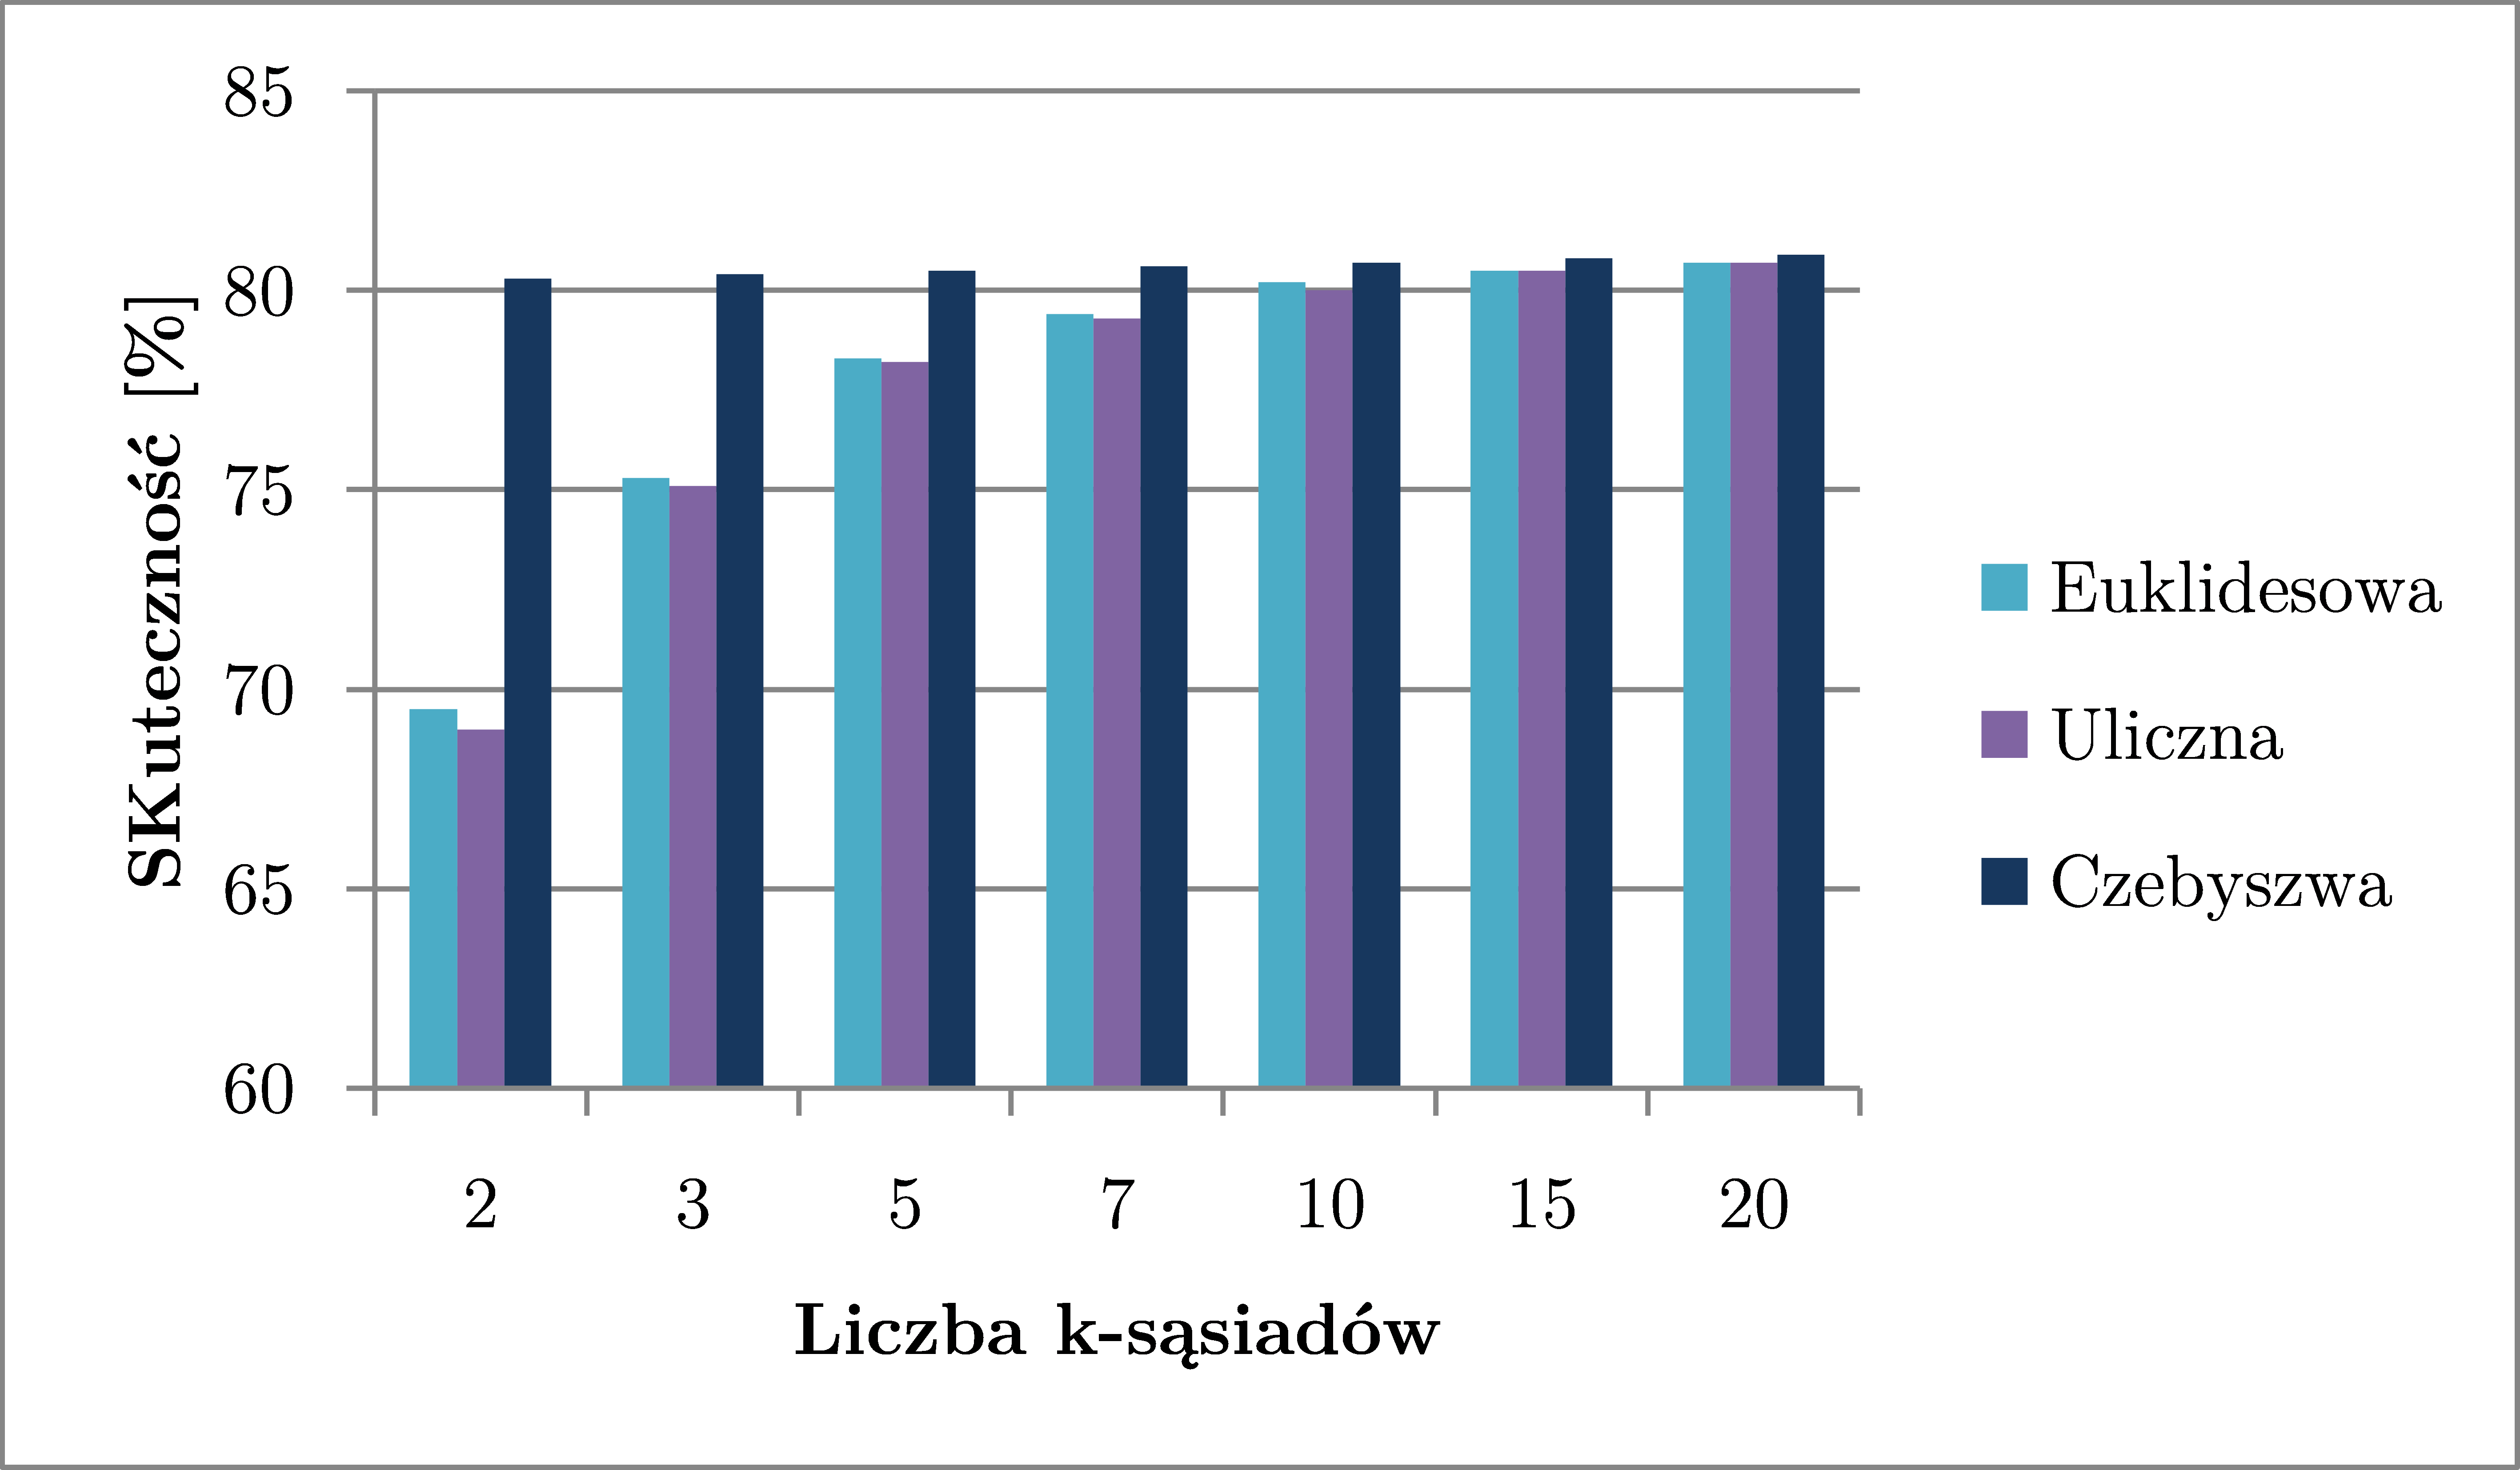
\includegraphics[width=0.9\textwidth]{{Rysunki/OWN-places.png}}
	\caption{Dane z Tabel 7-9 dla kategorii places}
\end{figure}

\begin{figure}[H]
	\centering
	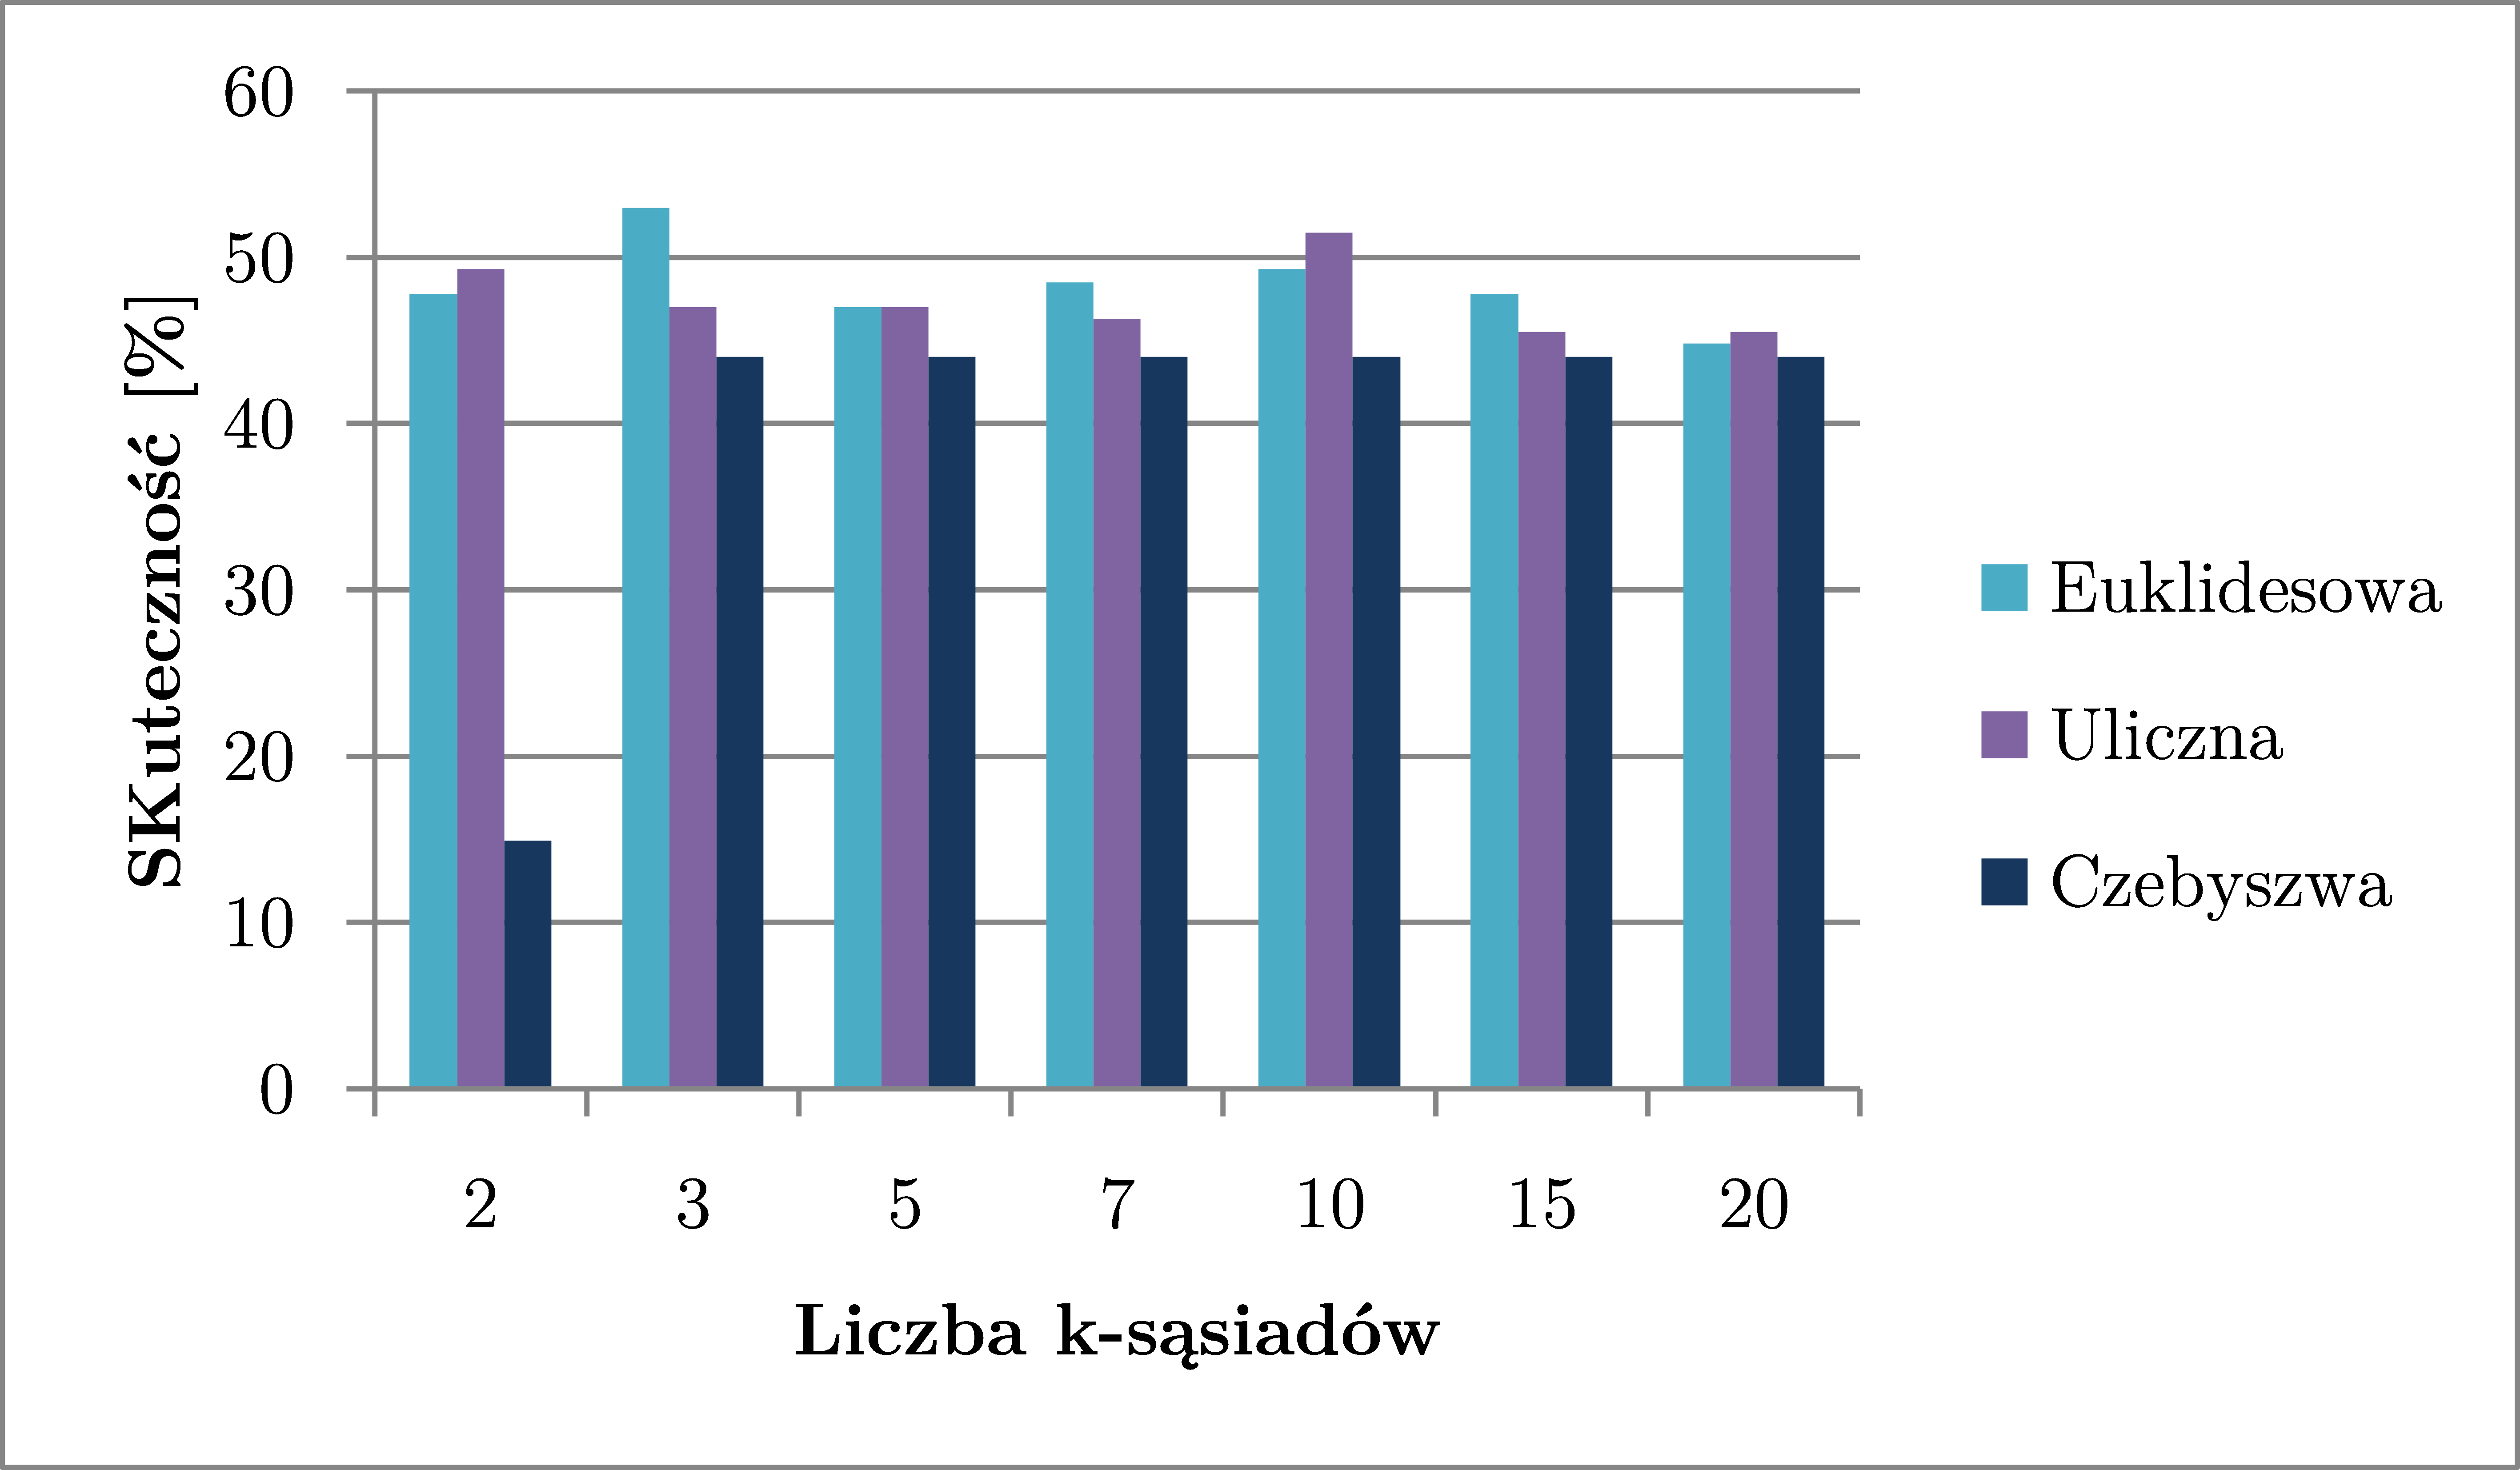
\includegraphics[width=0.9\textwidth]{{Rysunki/OWN-topics.png}}
	\caption{Dane z Tabel 7-9 dla kategorii topics}
\end{figure}

\begin{figure}[H]
	\centering
	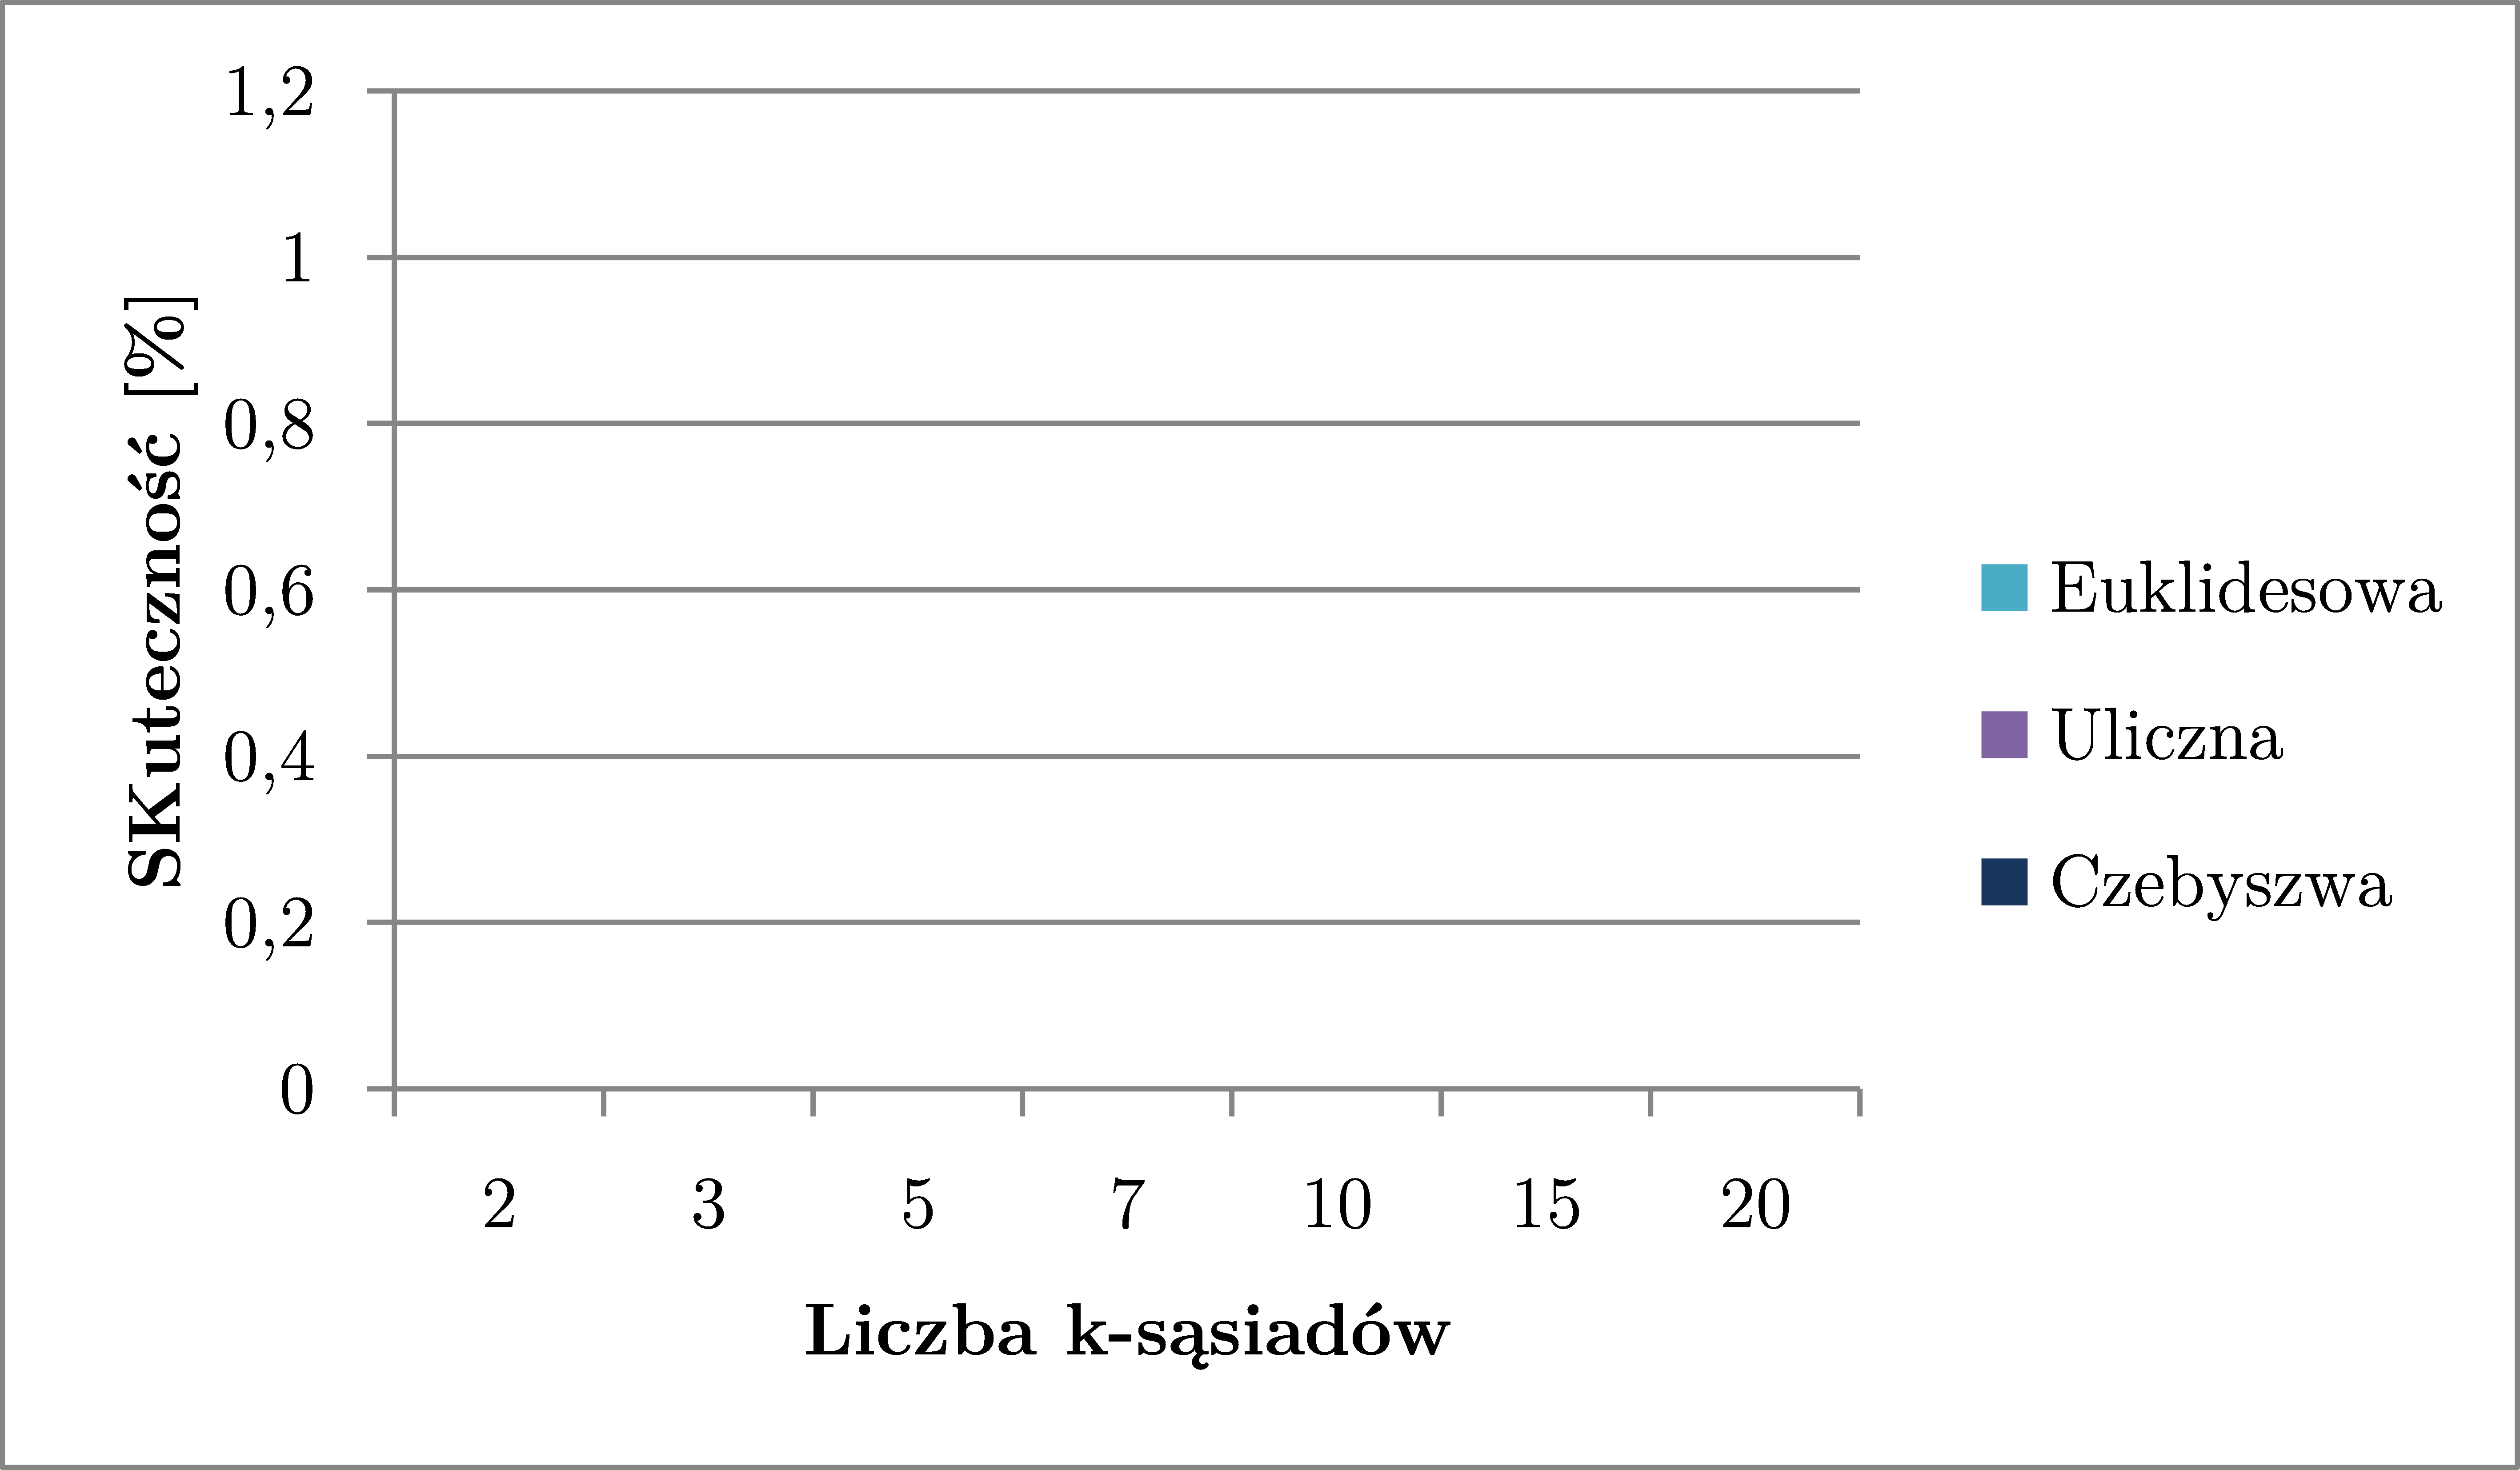
\includegraphics[width=0.9\textwidth]{{Rysunki/OWN-authors.png}}
	\caption{Dane z Tabel 7-9 dla kategorii authors (własne teksty)}
\end{figure}

\subsection{Wpływ podziału tekstów na zbiory treningowe i testowe na klasyfikację}

\begin{table}[H]
	\centering
	\begin{tabular}{c c c c} 
		\hline
		\textbf{k} & \textbf{80\%} & \textbf{60\%} &  \textbf{40\%} \\ [0.5ex] 
		\hline
		\hline 
		5 & 82.7 & 80.2 & 78.4 \\
		7 & 83.3 & 81.0 & 79.9 \\
		10 & 84.2 & 81.5 & 80.4 \\
		15 & 83.9 & 81.6 & 80.4 \\
		\hline
	\end{tabular}
	\caption{Skuteczność klasyfikacji dla pierwszego sposobu ekstrakcji, dla kategorii places}
\end{table}

\begin{figure}[H]
	\centering
	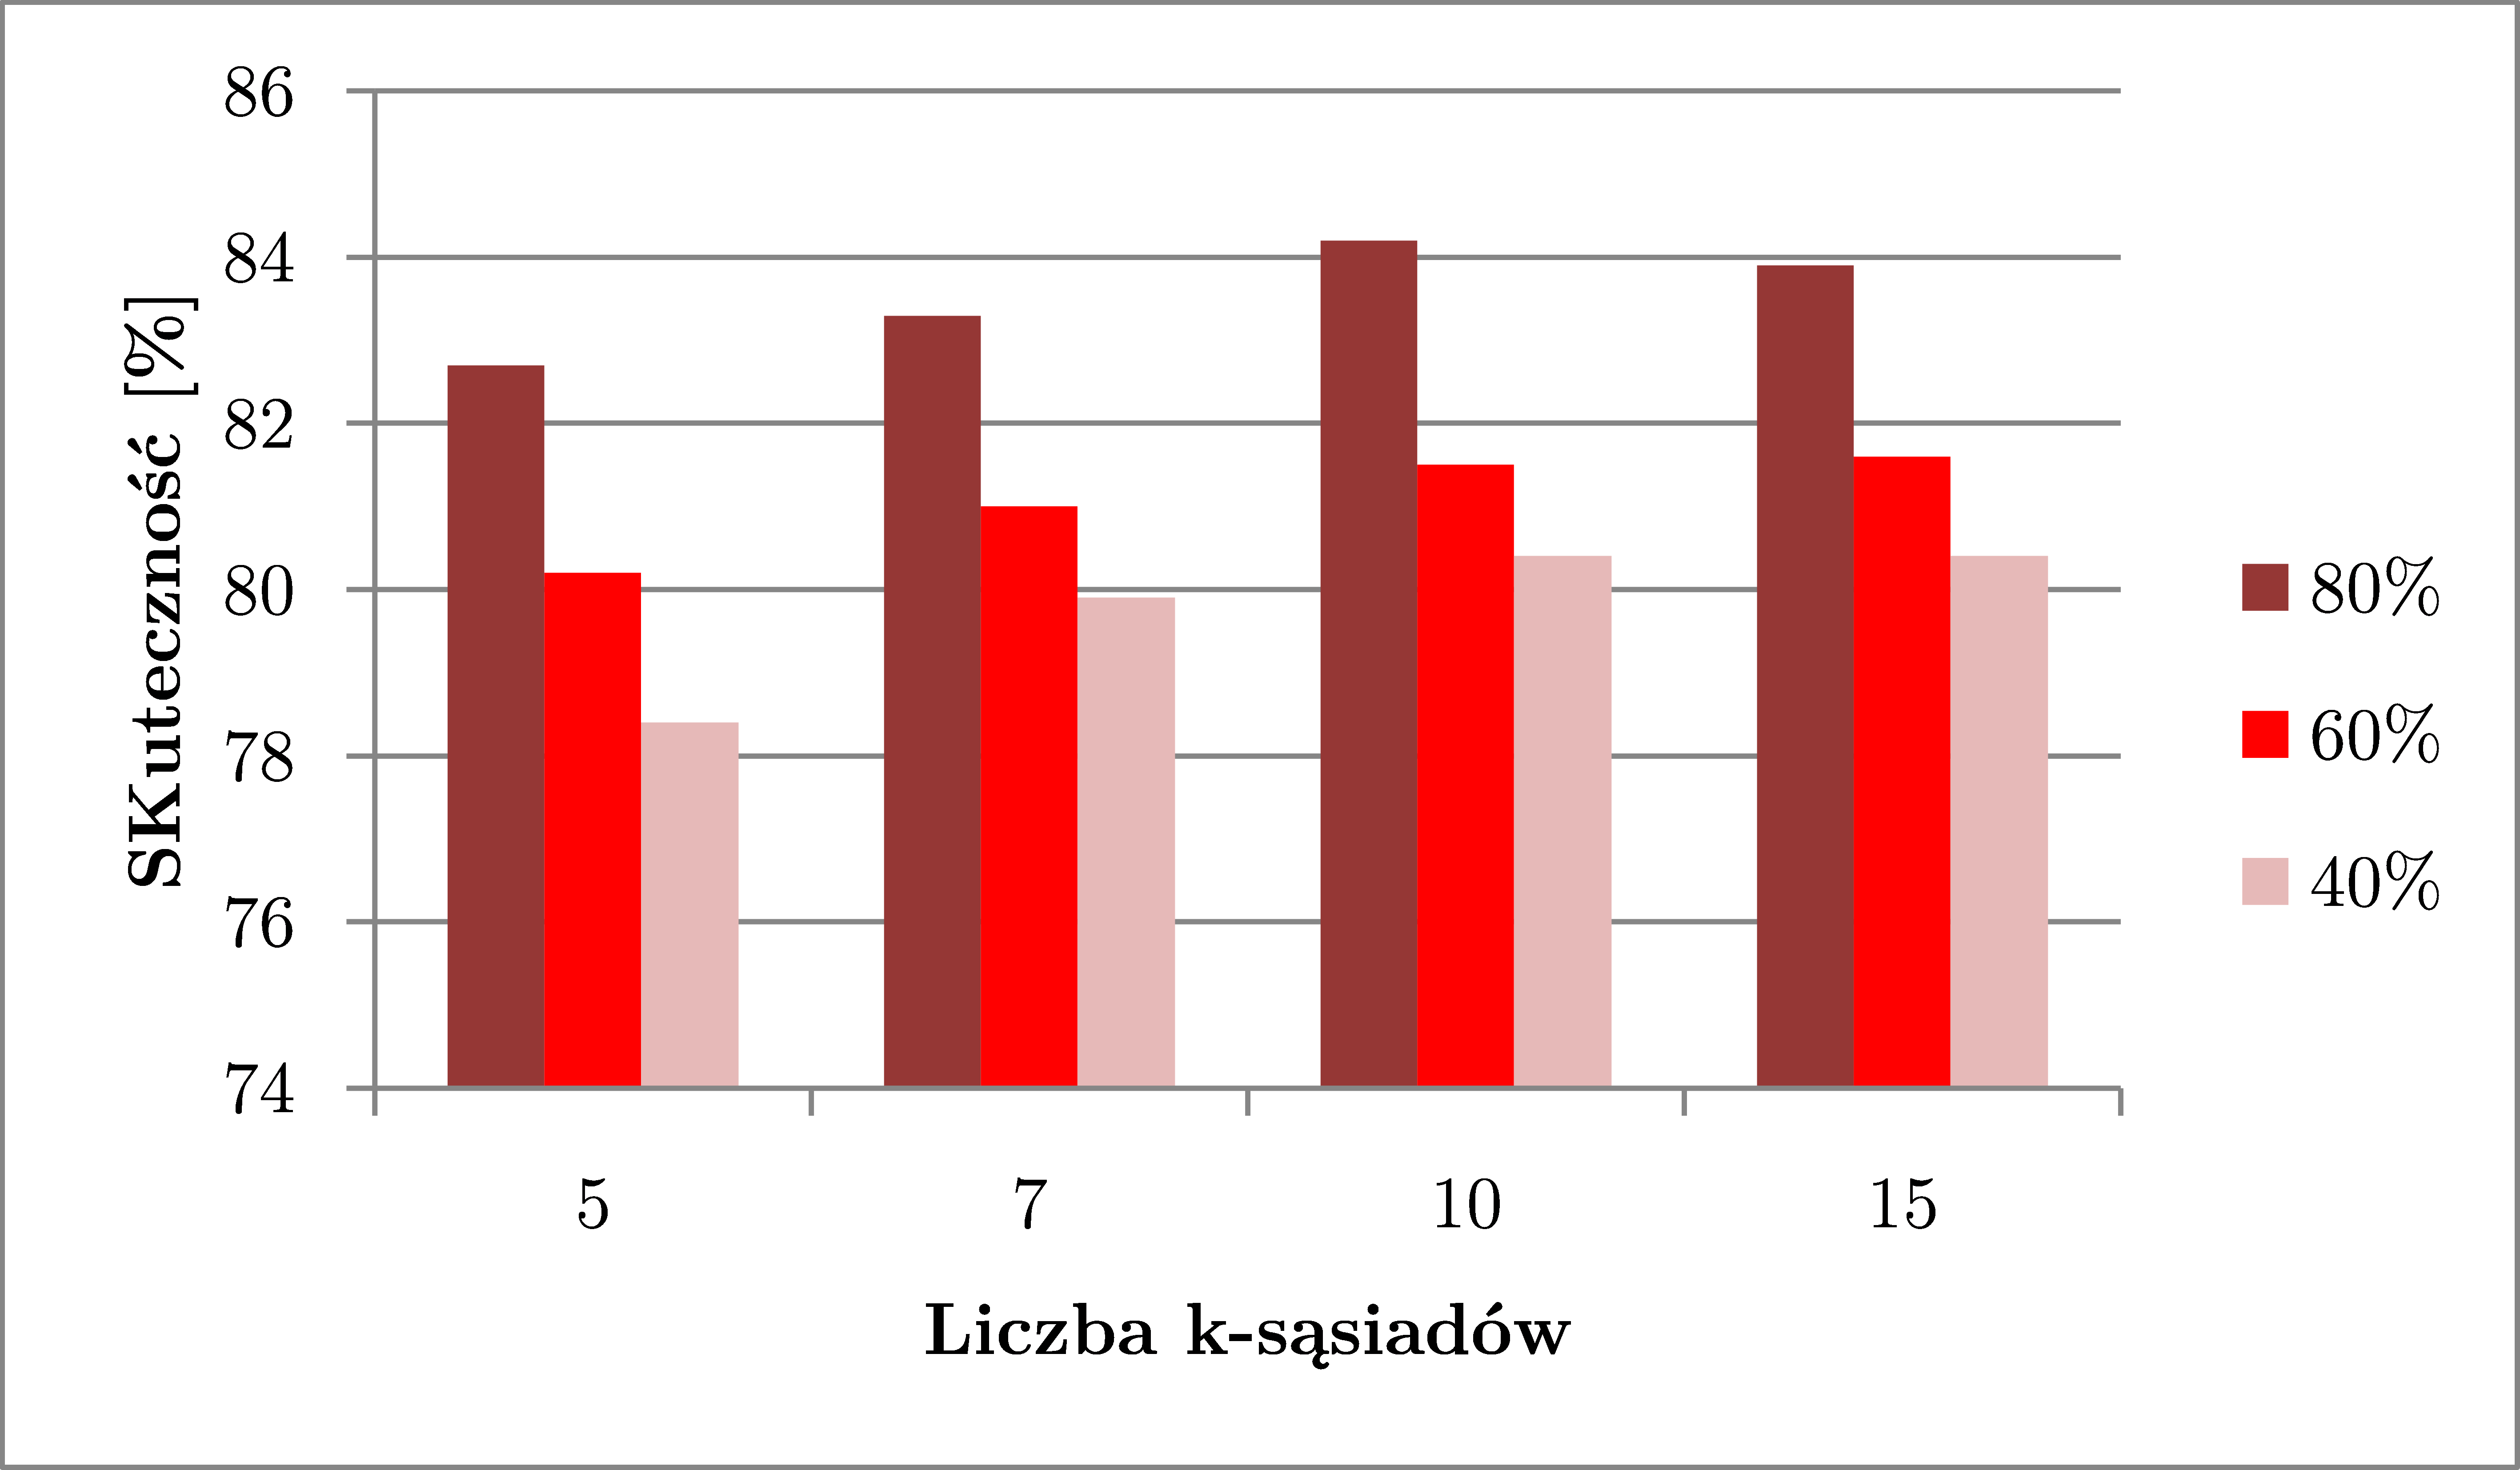
\includegraphics[width=0.9\textwidth]{{Rysunki/TF-80-60-40-places.png}}
	\caption{Skuteczność klasyfikacji dla pierwszego sposobu ekstrakcji, dla kategorii places}
\end{figure}

\begin{table}[H]
	\centering
	\begin{tabular}{c c c c} 
		\hline
		\textbf{k} & \textbf{80\%} & \textbf{60\%} &  \textbf{40\%} \\ [0.5ex] 
		\hline
		\hline 
		7 & 56.7 & 53.7 & 62.7 \\
		10 & 59.7 & 60.4 & 62.2 \\
		15 & 58.2 & 62.7 & 64.7 \\
		20 & 62.7 & 61.2 & 64.7 \\
		\hline
	\end{tabular}
	\caption{Skuteczność klasyfikacji dla pierwszego sposobu ekstrakcji, dla kategorii topics}
\end{table}

\begin{figure}[H]
	\centering
	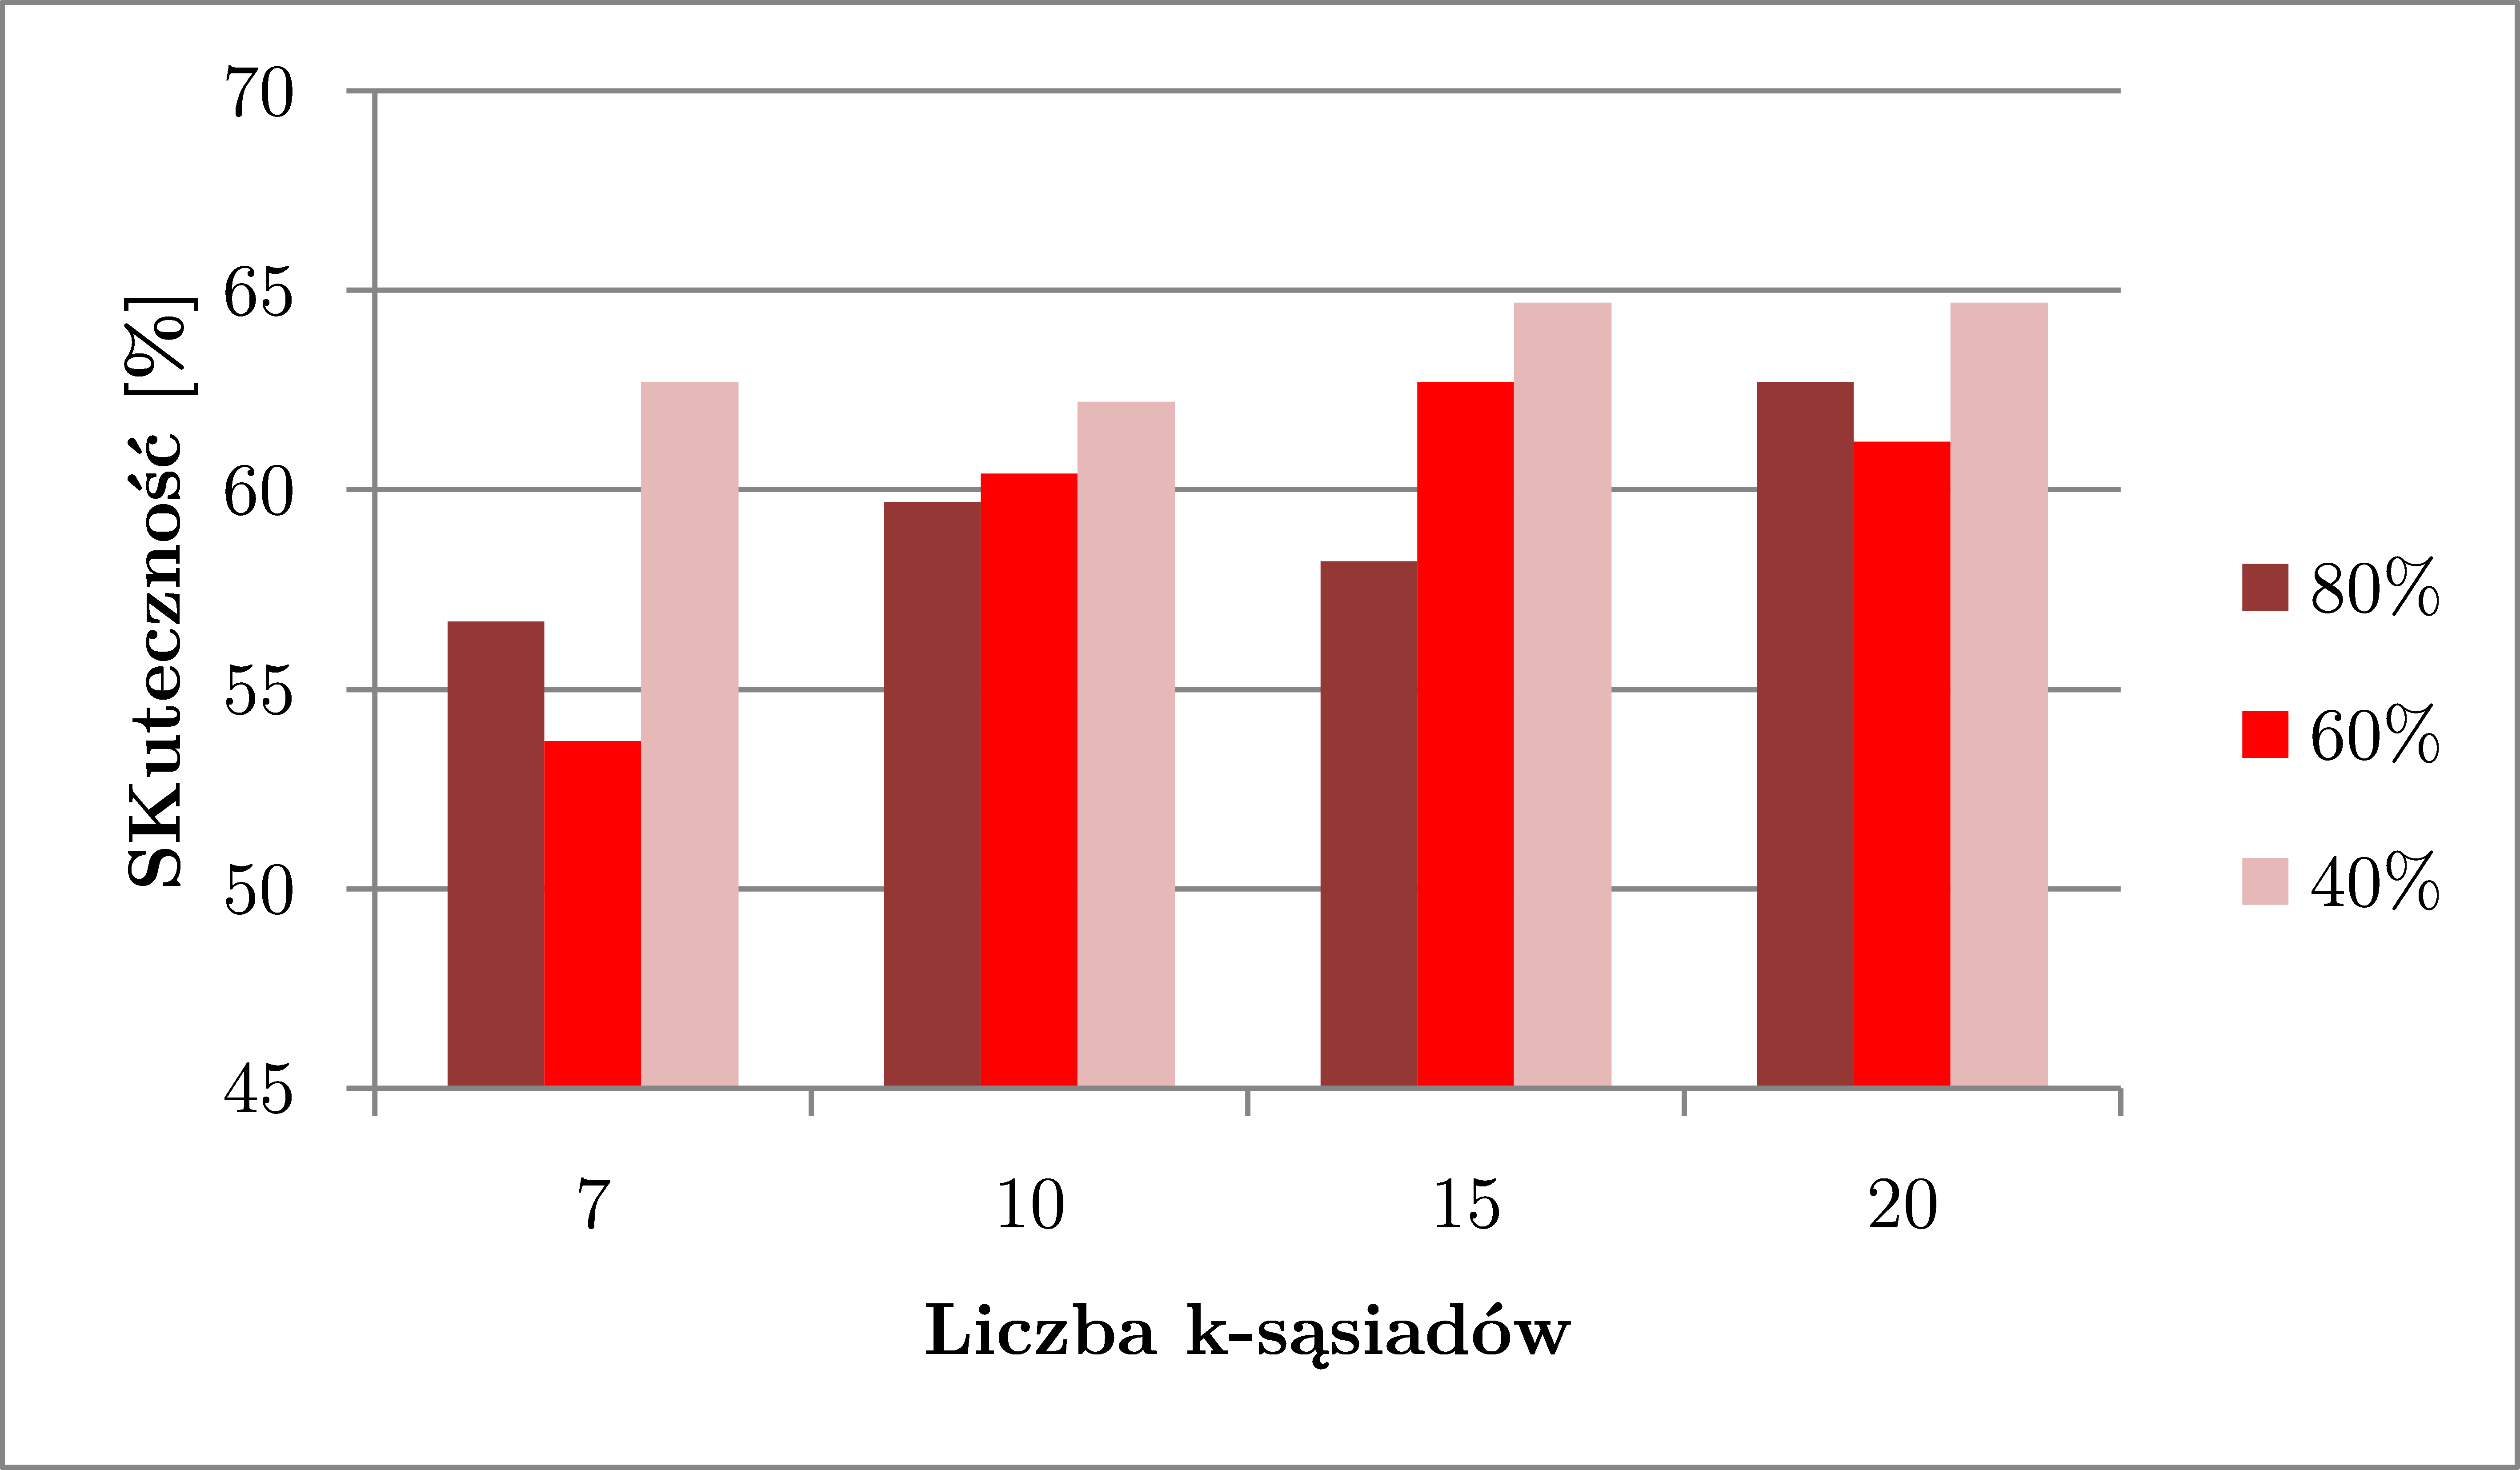
\includegraphics[width=0.9\textwidth]{{Rysunki/TF-80-60-40-topics.png}}
	\caption{Skuteczność klasyfikacji dla pierwszego sposobu ekstrakcji, dla kategorii topics}
\end{figure}

\begin{table}[H]
	\centering
	\begin{tabular}{c c c c} 
		\hline
		\textbf{k} & \textbf{80\%} & \textbf{60\%} &  \textbf{40\%} \\ [0.5ex] 
		\hline
		\hline 
		2 & 19.0 & 43.9 & 38.7 \\
		3 & 19.0 & 43.9 & 37.1 \\
		5 & 23.8 & 36.6 & 29.0 \\
		7 & 14.3 & 26.8 & 32.3 \\
		\hline
	\end{tabular}
	\caption{Skuteczność klasyfikacji dla pierwszego sposobu ekstrakcji, dla kategorii authors}
\end{table}

\begin{figure}[H]
	\centering
	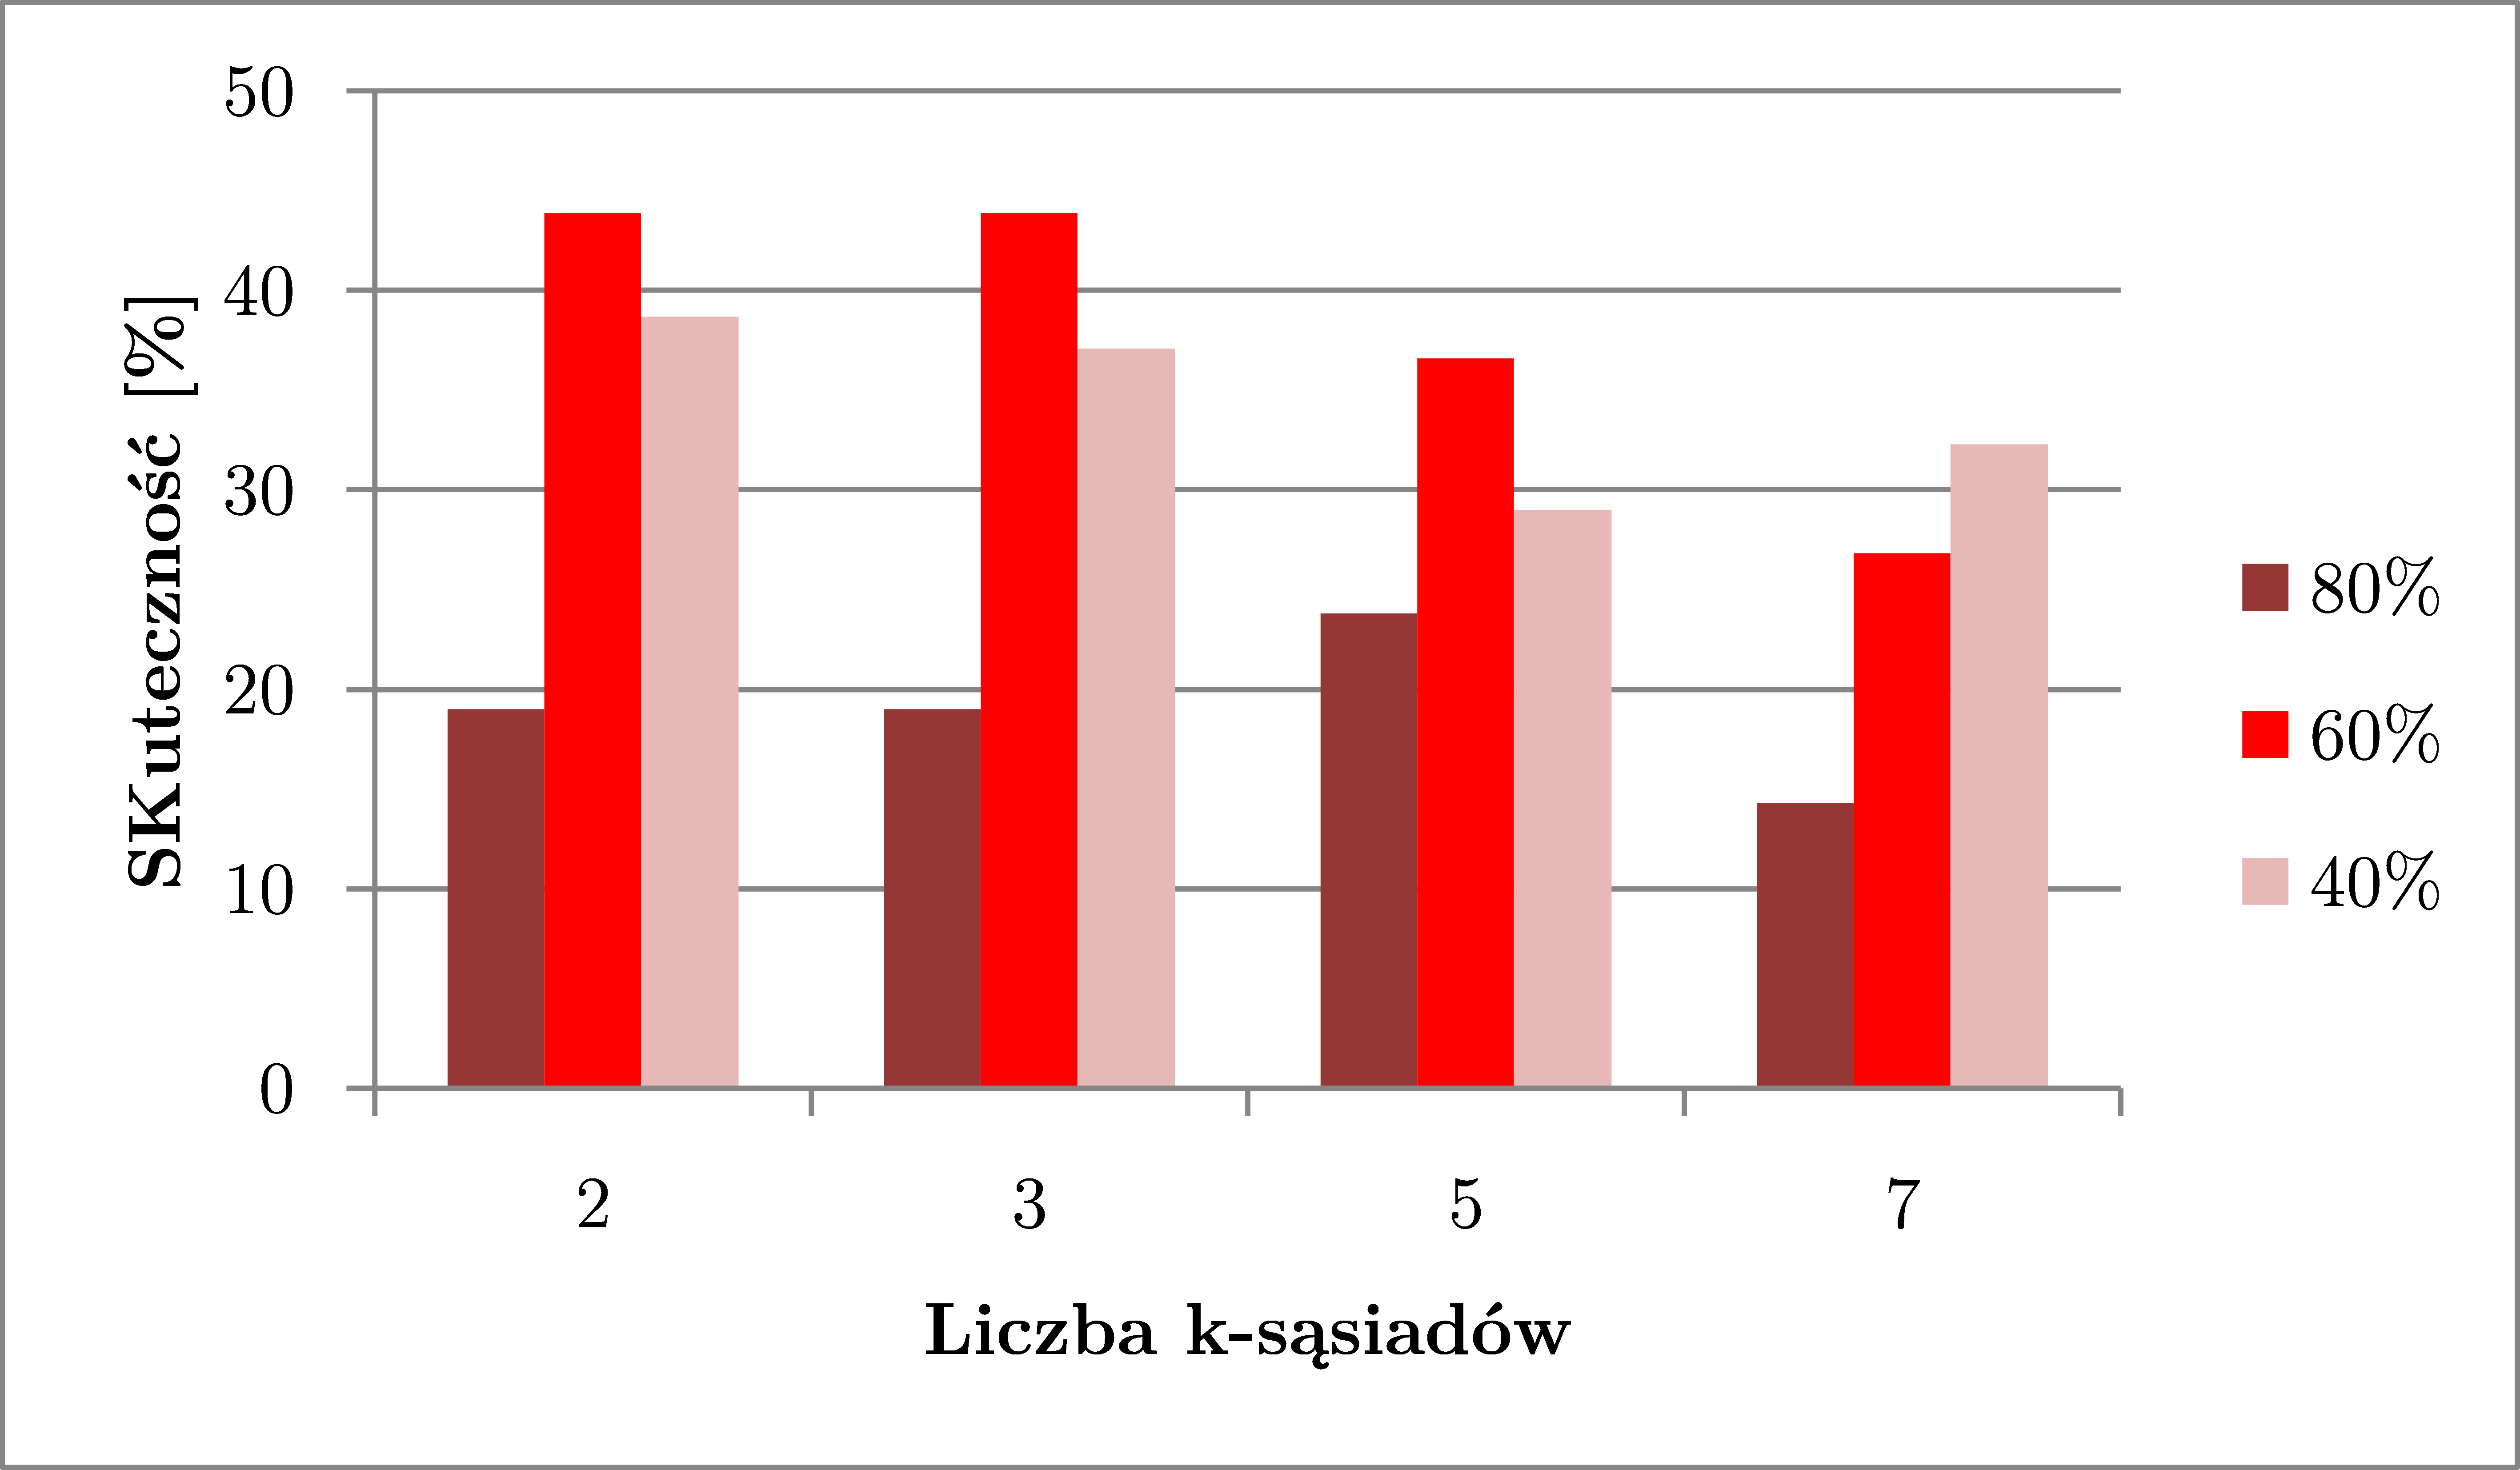
\includegraphics[width=0.9\textwidth]{{Rysunki/TF-80-60-40-authors.png}}
	\caption{Skuteczność klasyfikacji dla pierwszego sposobu ekstrakcji, dla kategorii authors}
\end{figure}


\begin{table}[H]
	\centering
	\begin{tabular}{c c c c} 
		\hline
		\textbf{k} & \textbf{80\%} & \textbf{60\%} &  \textbf{40\%} \\ [0.5ex]
		\hline
		\hline 
		7 & 82.6 & 79.4 & 78.5 \\
		10 & 83.1 & 80.2 & 79.2 \\
		15 & 83.5 & 80.5 & 79.6 \\
		20 & 83.3 & 80.7 & 79.7 \\
		\hline
	\end{tabular}
	\caption{Skuteczność klasyfikacji dla drugiego sposobu ekstrakcji, dla kategorii places}
\end{table}

\begin{figure}[H]
	\centering
	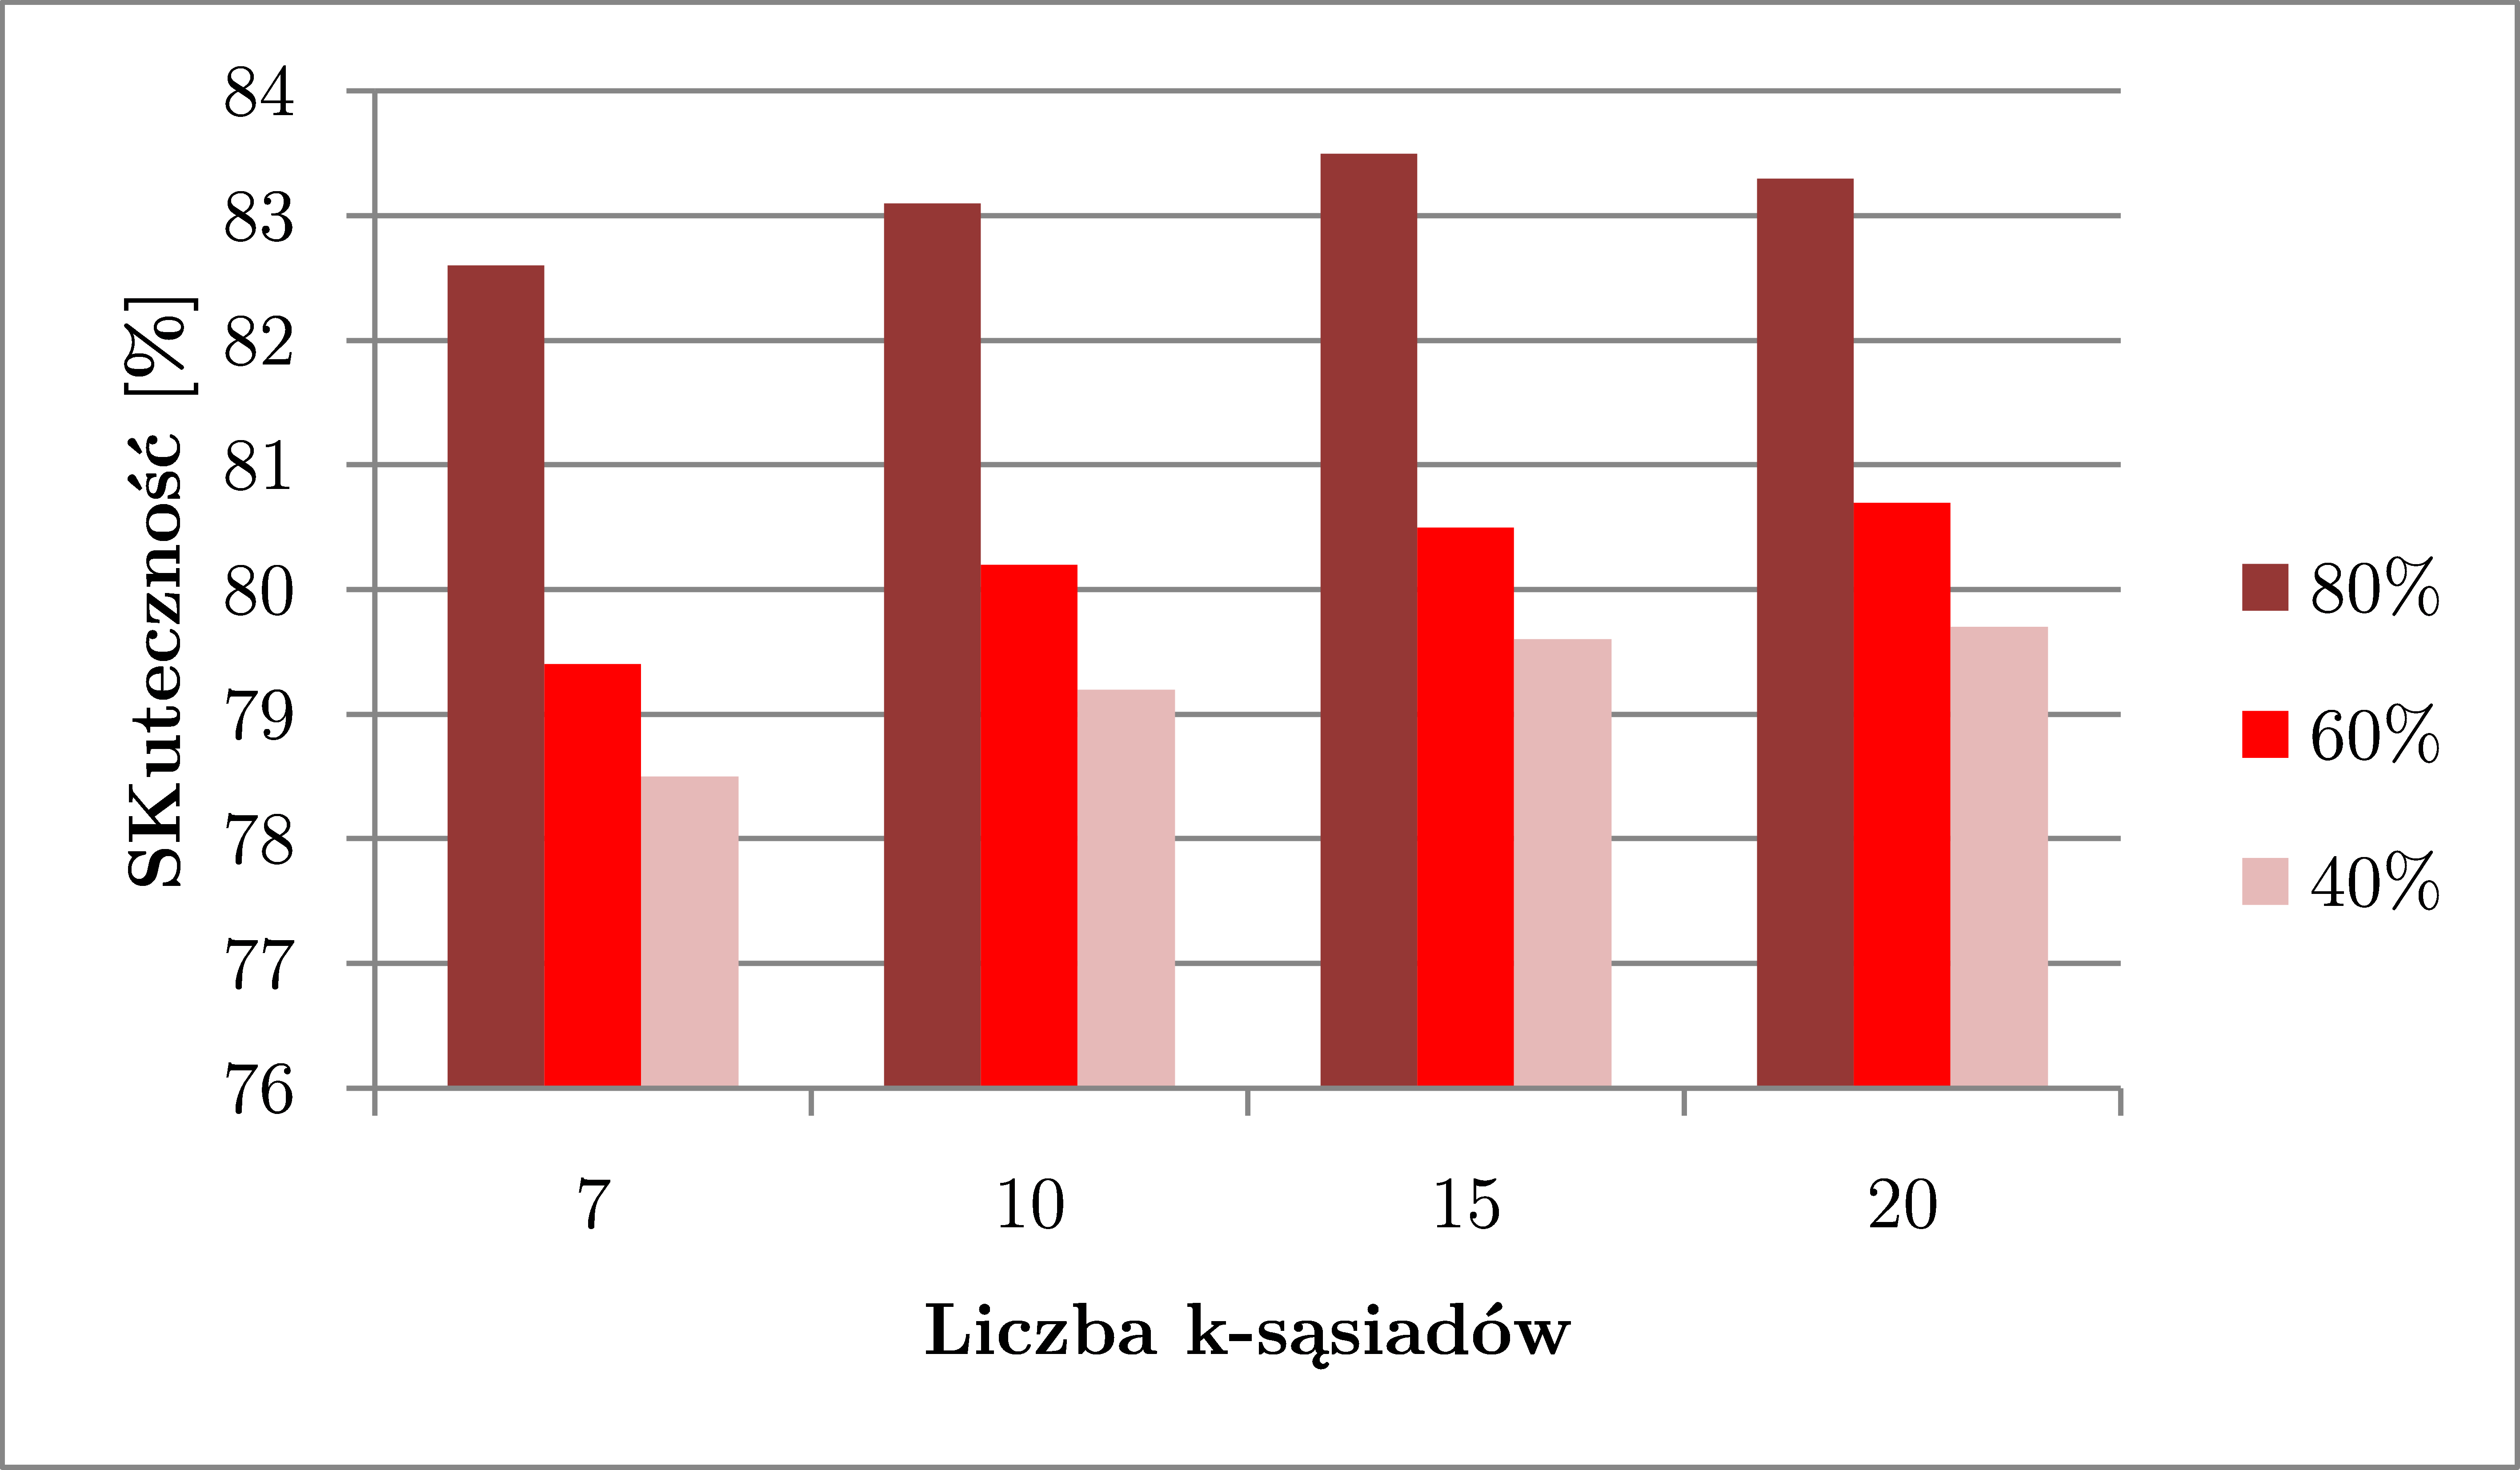
\includegraphics[width=0.9\textwidth]{{Rysunki/OWN-80-60-40-places.png}}
	\caption{Skuteczność klasyfikacji dla drugiego sposobu ekstrakcji, dla kategorii places}
\end{figure}

\begin{table}[H]
	\centering
	\begin{tabular}{c c c c} 
		\hline
		\textbf{k} & \textbf{80\%} & \textbf{60\%} &  \textbf{40\%} \\ [0.5ex]
		\hline
		\hline 
		3 & 55.2 & 53.0 & 43.3 \\
		5 & 55.2 & 47.0 & 43.8 \\
		7 & 55.2 & 48.5 & 42.3 \\
		10 & 55.2 & 49.3 & 40.8 \\
		\hline
	\end{tabular}
	\caption{Skuteczność klasyfikacji dla trzeciego sposobu ekstrakcji, dla kategorii topics}
\end{table}

\begin{figure}[H]
	\centering
	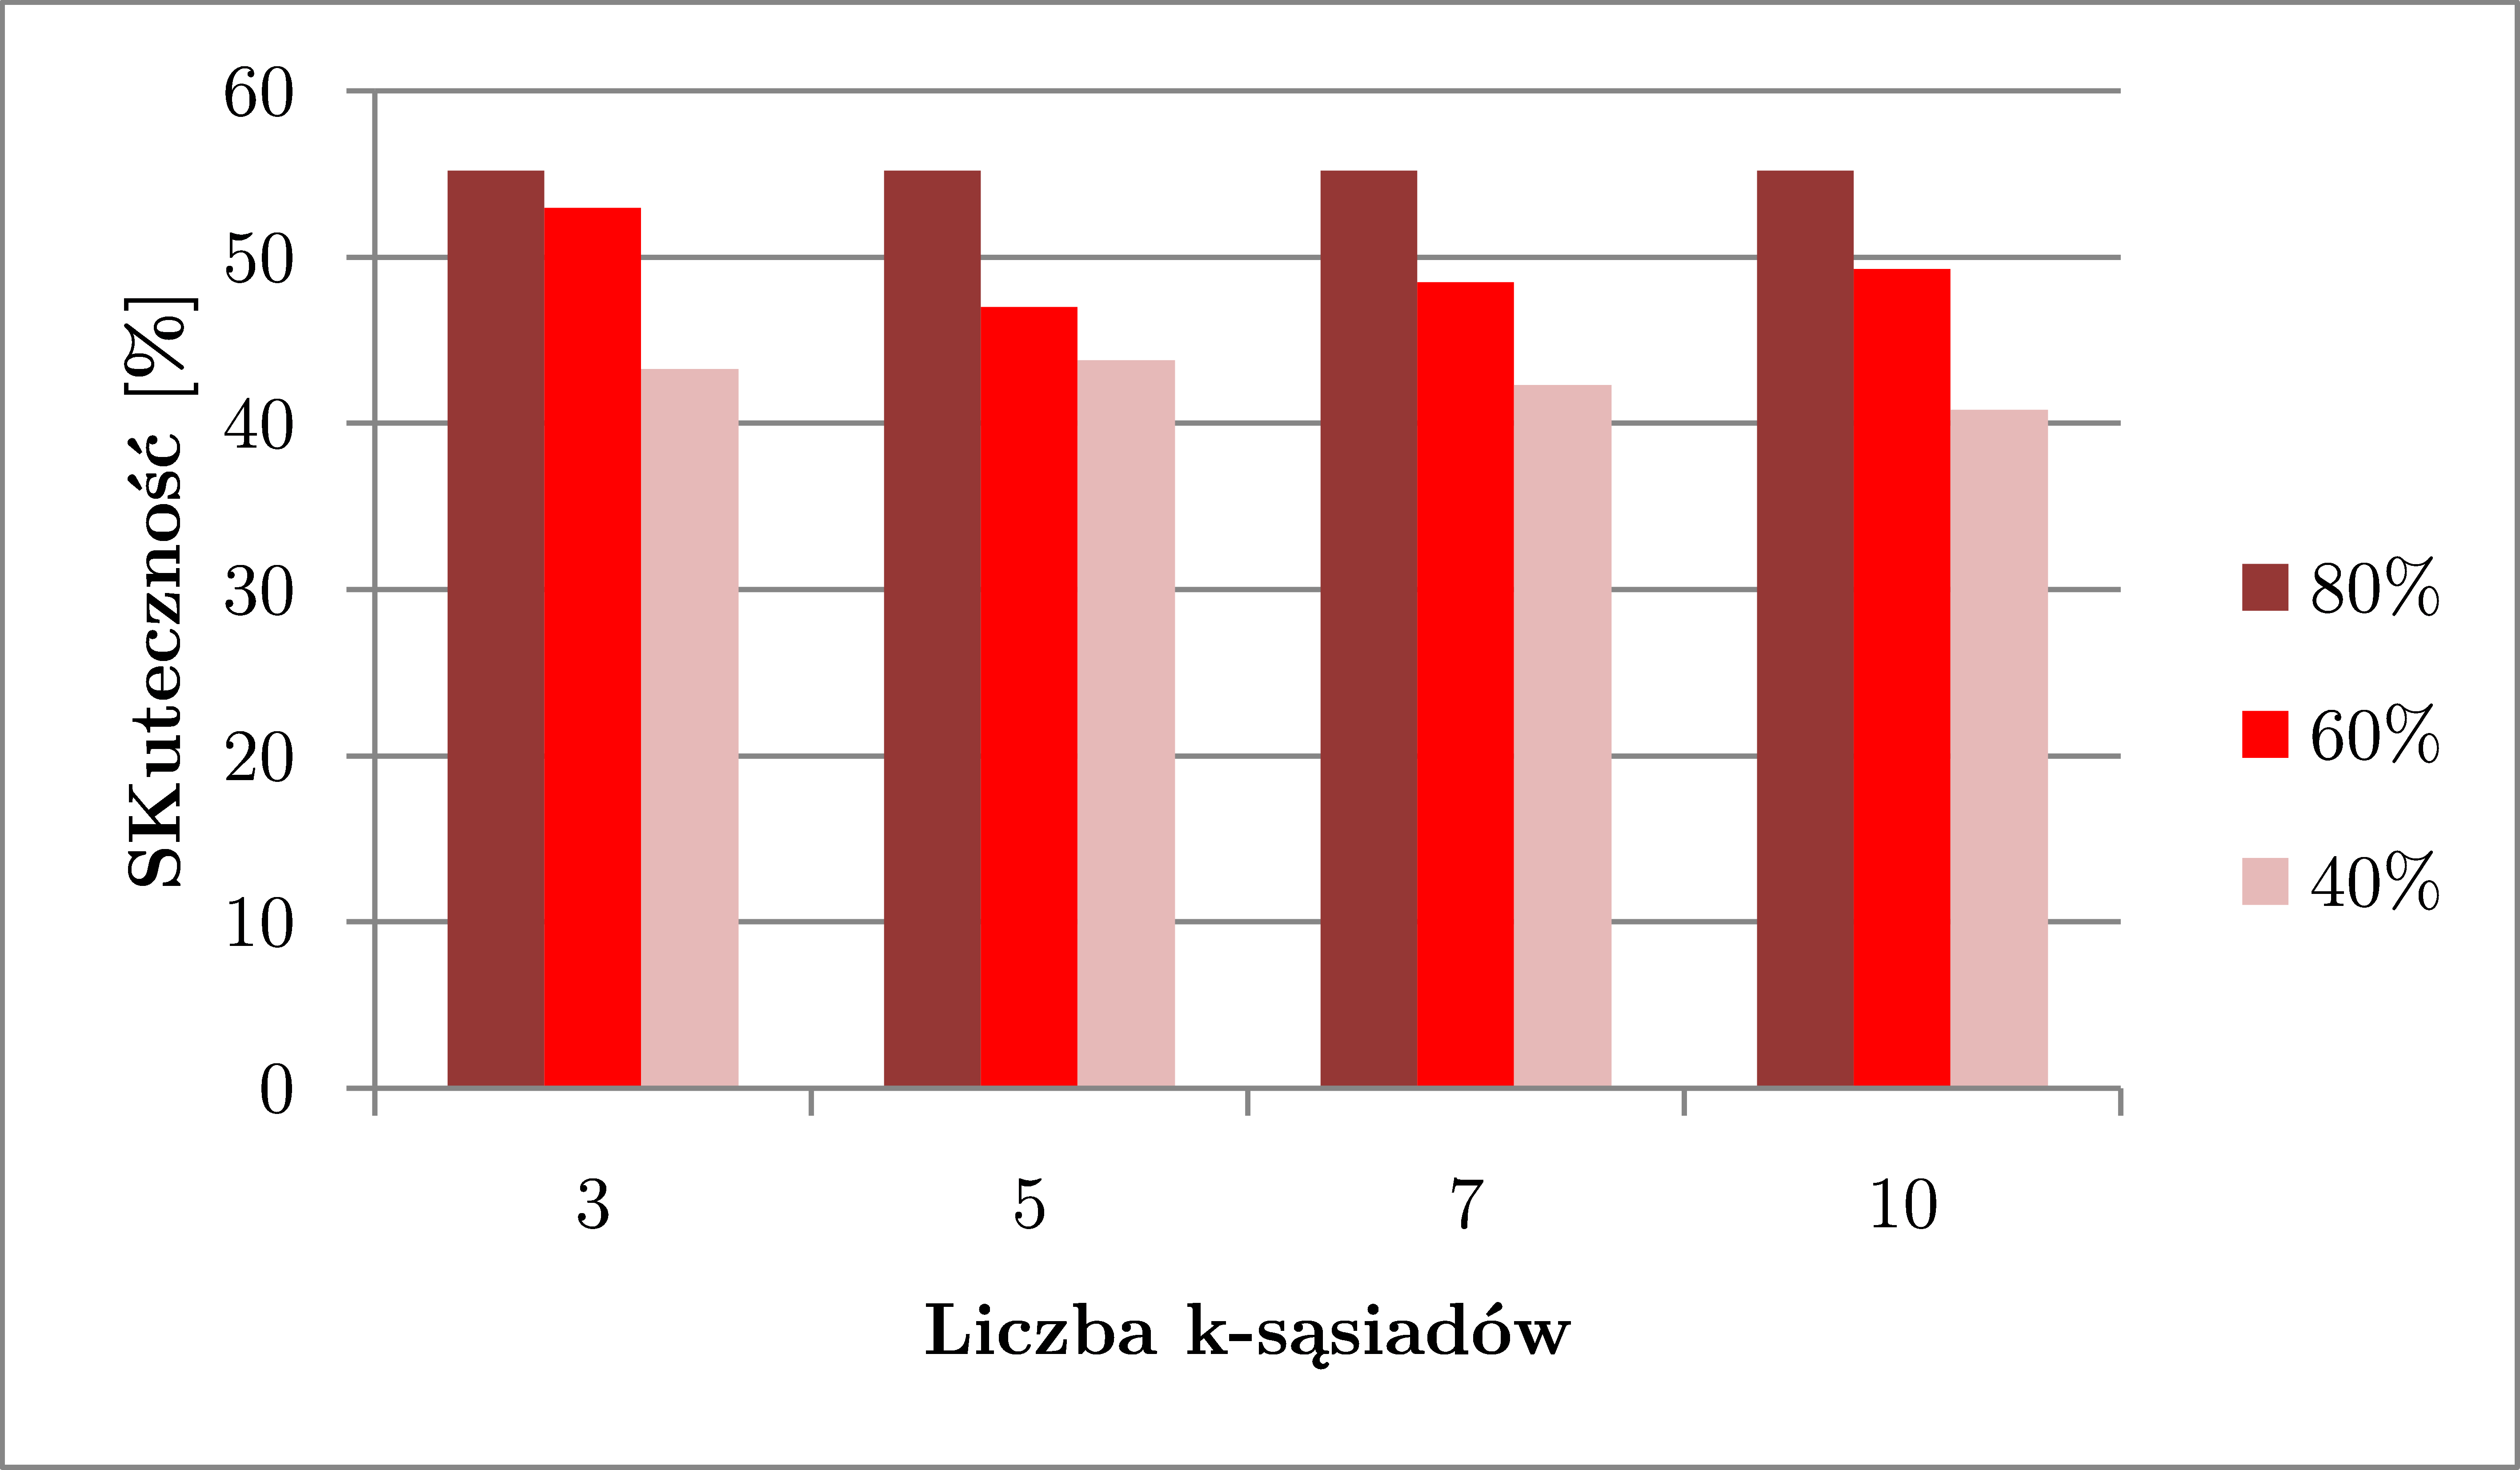
\includegraphics[width=0.9\textwidth]{{Rysunki/OWN-80-60-40-topics.png}}
	\caption{Skuteczność klasyfikacji dla trzeciego sposobu ekstrakcji, dla kategorii topics}
\end{figure}

\begin{table}[H]
	\centering
	\begin{tabular}{c c c c} 
		\hline
		\textbf{k} & \textbf{80\%} & \textbf{60\%} &  \textbf{40\%} \\ [0.5ex]
		\hline
		\hline 
		7 & 71.4 & 63.4 & 46.8 \\
		10 & 66.7 & 63.4 & 48.4 \\
		15 & 71.4 & 58.5 & 50.0 \\
		20 & 71.4 & 53.7 &  33.9 \\
		\hline
	\end{tabular}
	\caption{Skuteczność klasyfikacji dla trzeciego sposobu ekstrakcji, dla kategorii authors}
\end{table}

\begin{figure}[H]
	\centering
	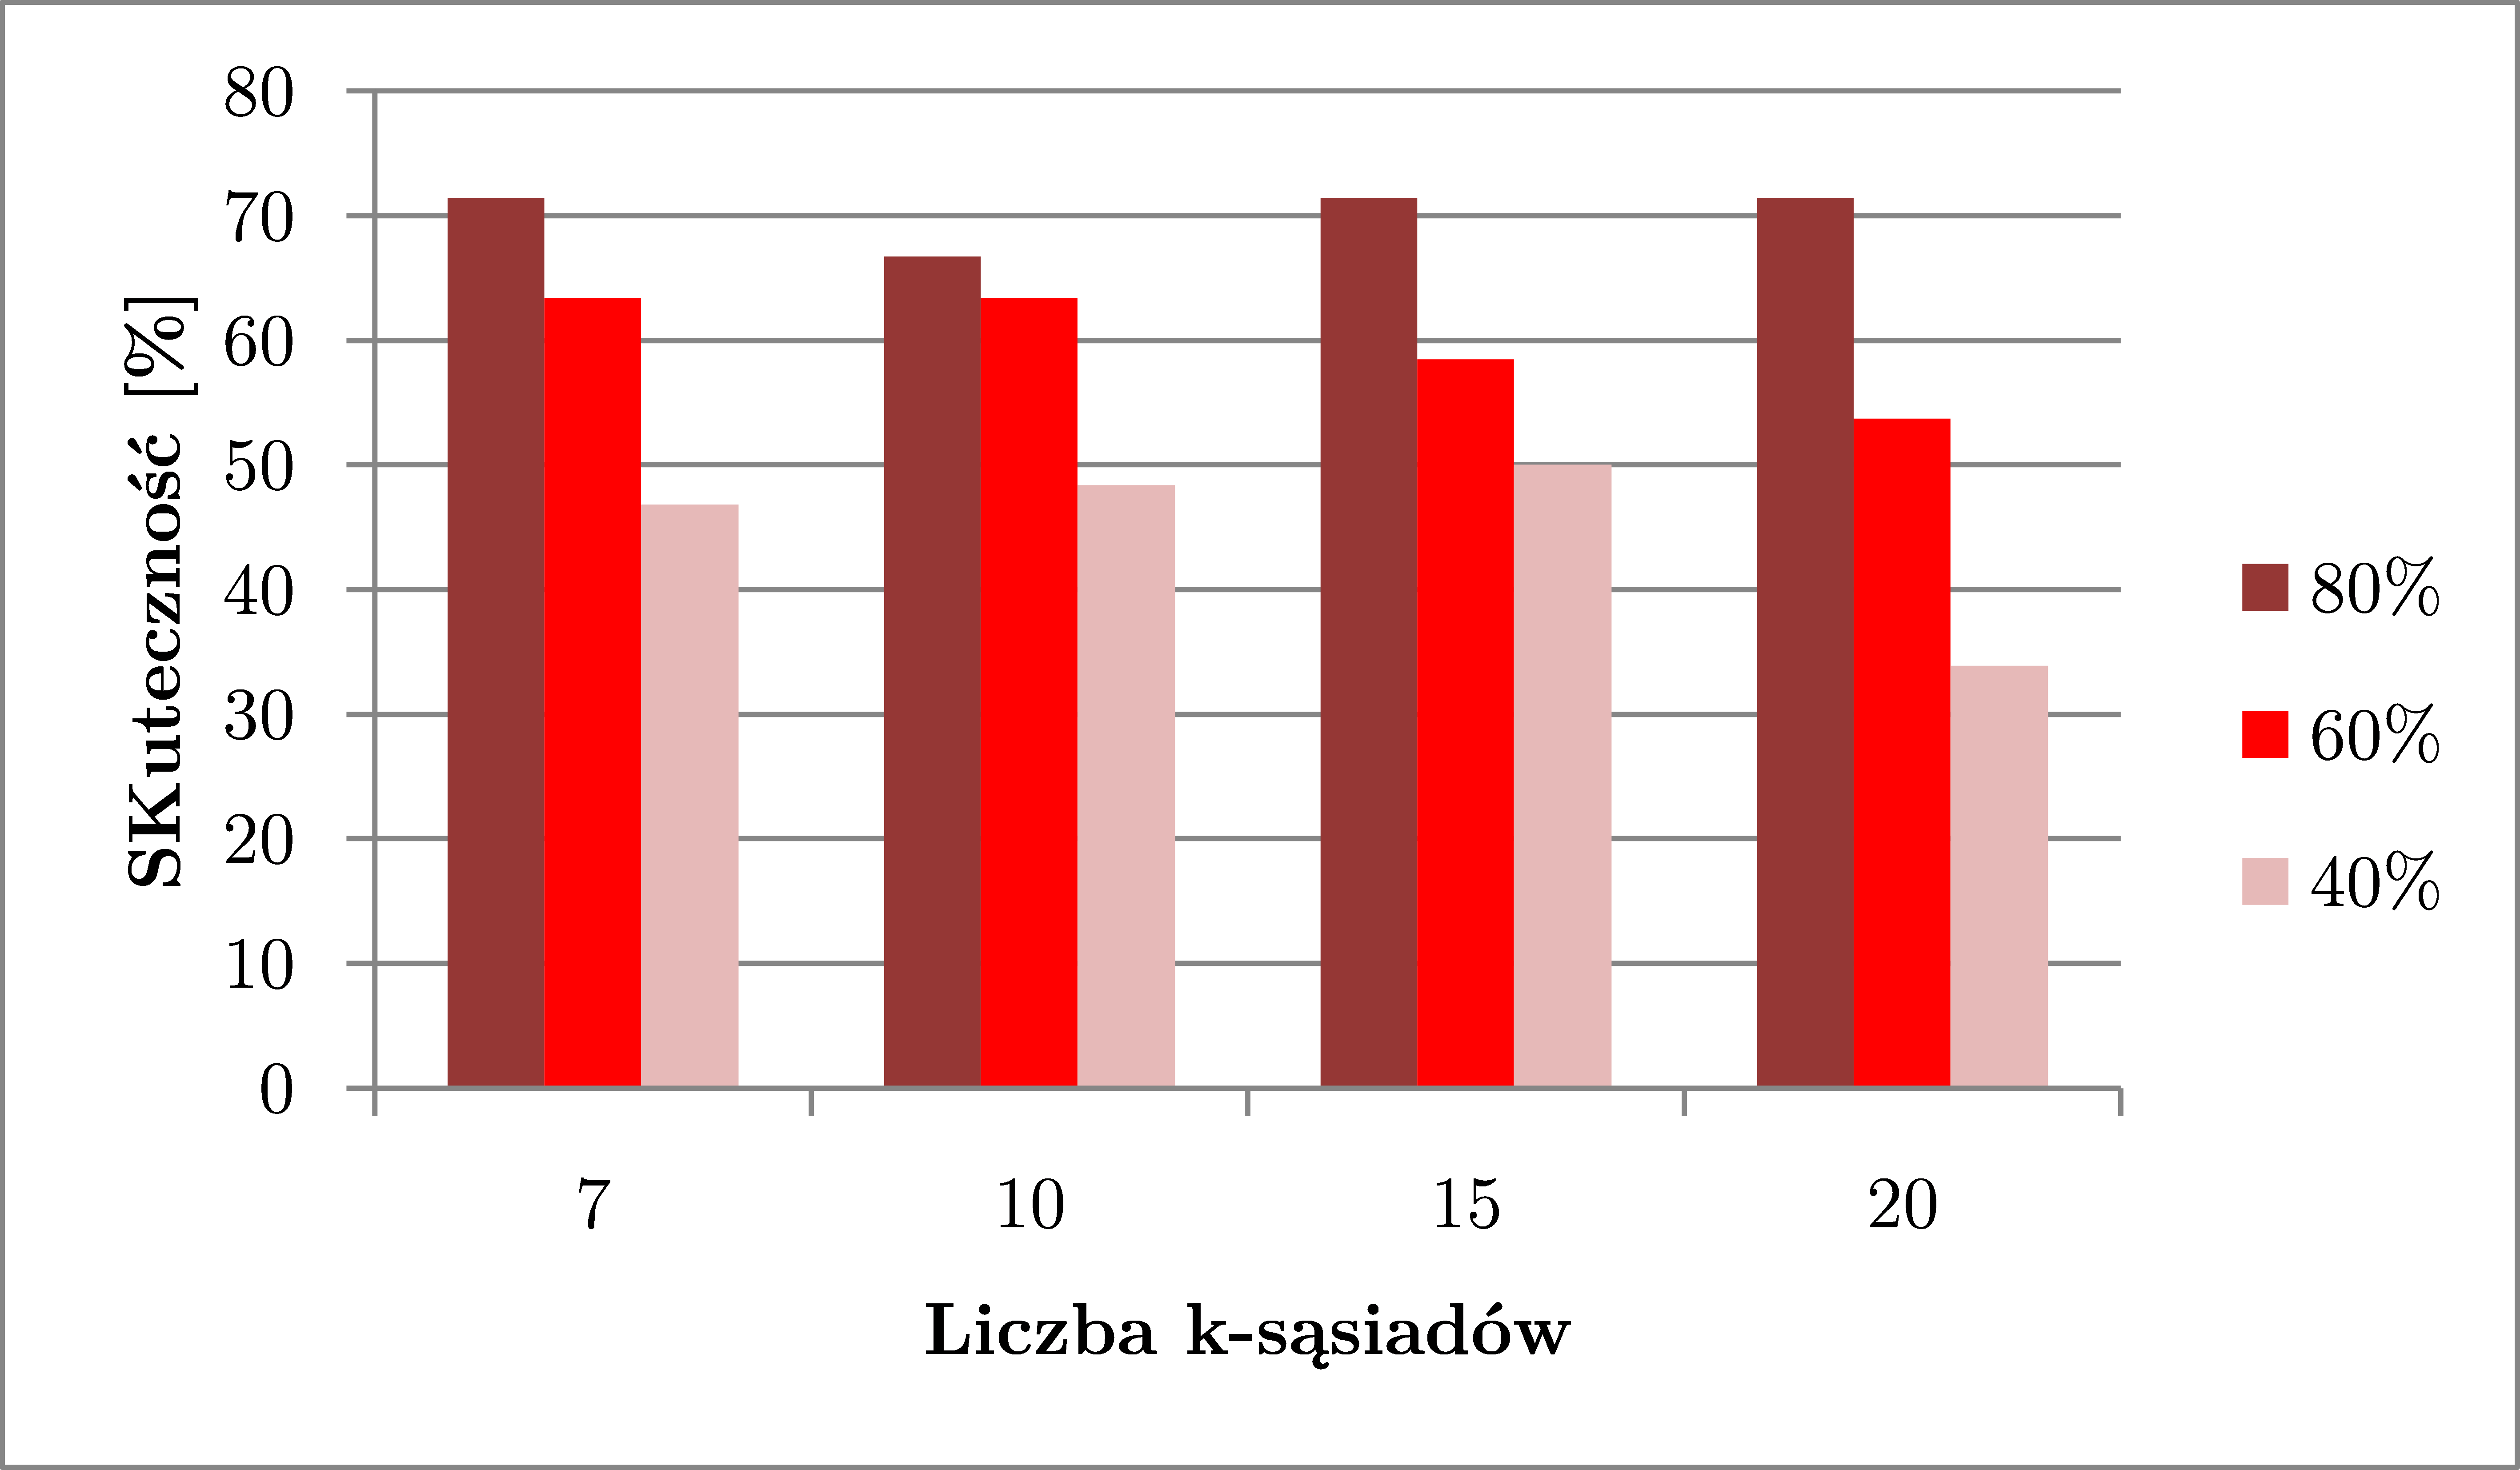
\includegraphics[width=0.9\textwidth]{{Rysunki/OWN-80-60-40-authors.png}}
	\caption{Skuteczność klasyfikacji dla trzeciego sposobu ekstrakcji, dla kategorii authors}
\end{figure}

\subsection{Wpływ konkretnych cech na klasyfikację}

Na wykresach widoczne są następujące oznaczenia:
\begin{description}
	\item [$c_{1})$] Liczba słów,
	\item [$c_{2})$] Liczba słów, których długość nie przekracza 3 znaków,
	\item [$c_{3})$] Liczba słów, których długość zawiera się w zakresie 4-7 znaków,
	\item [$c_{4})$] Liczba słów, których długość przekracza 8 znaków,
	\item [$c_{5})$] Liczba unikalnych słów,
	\item [$c_{6})$] Liczba słów napisanych wielką literą,
	\item [$c_{7})$] liczba słów rozpoczynających się wielką literą. 
\end{description}

\begin{figure}[H]
	\centering
	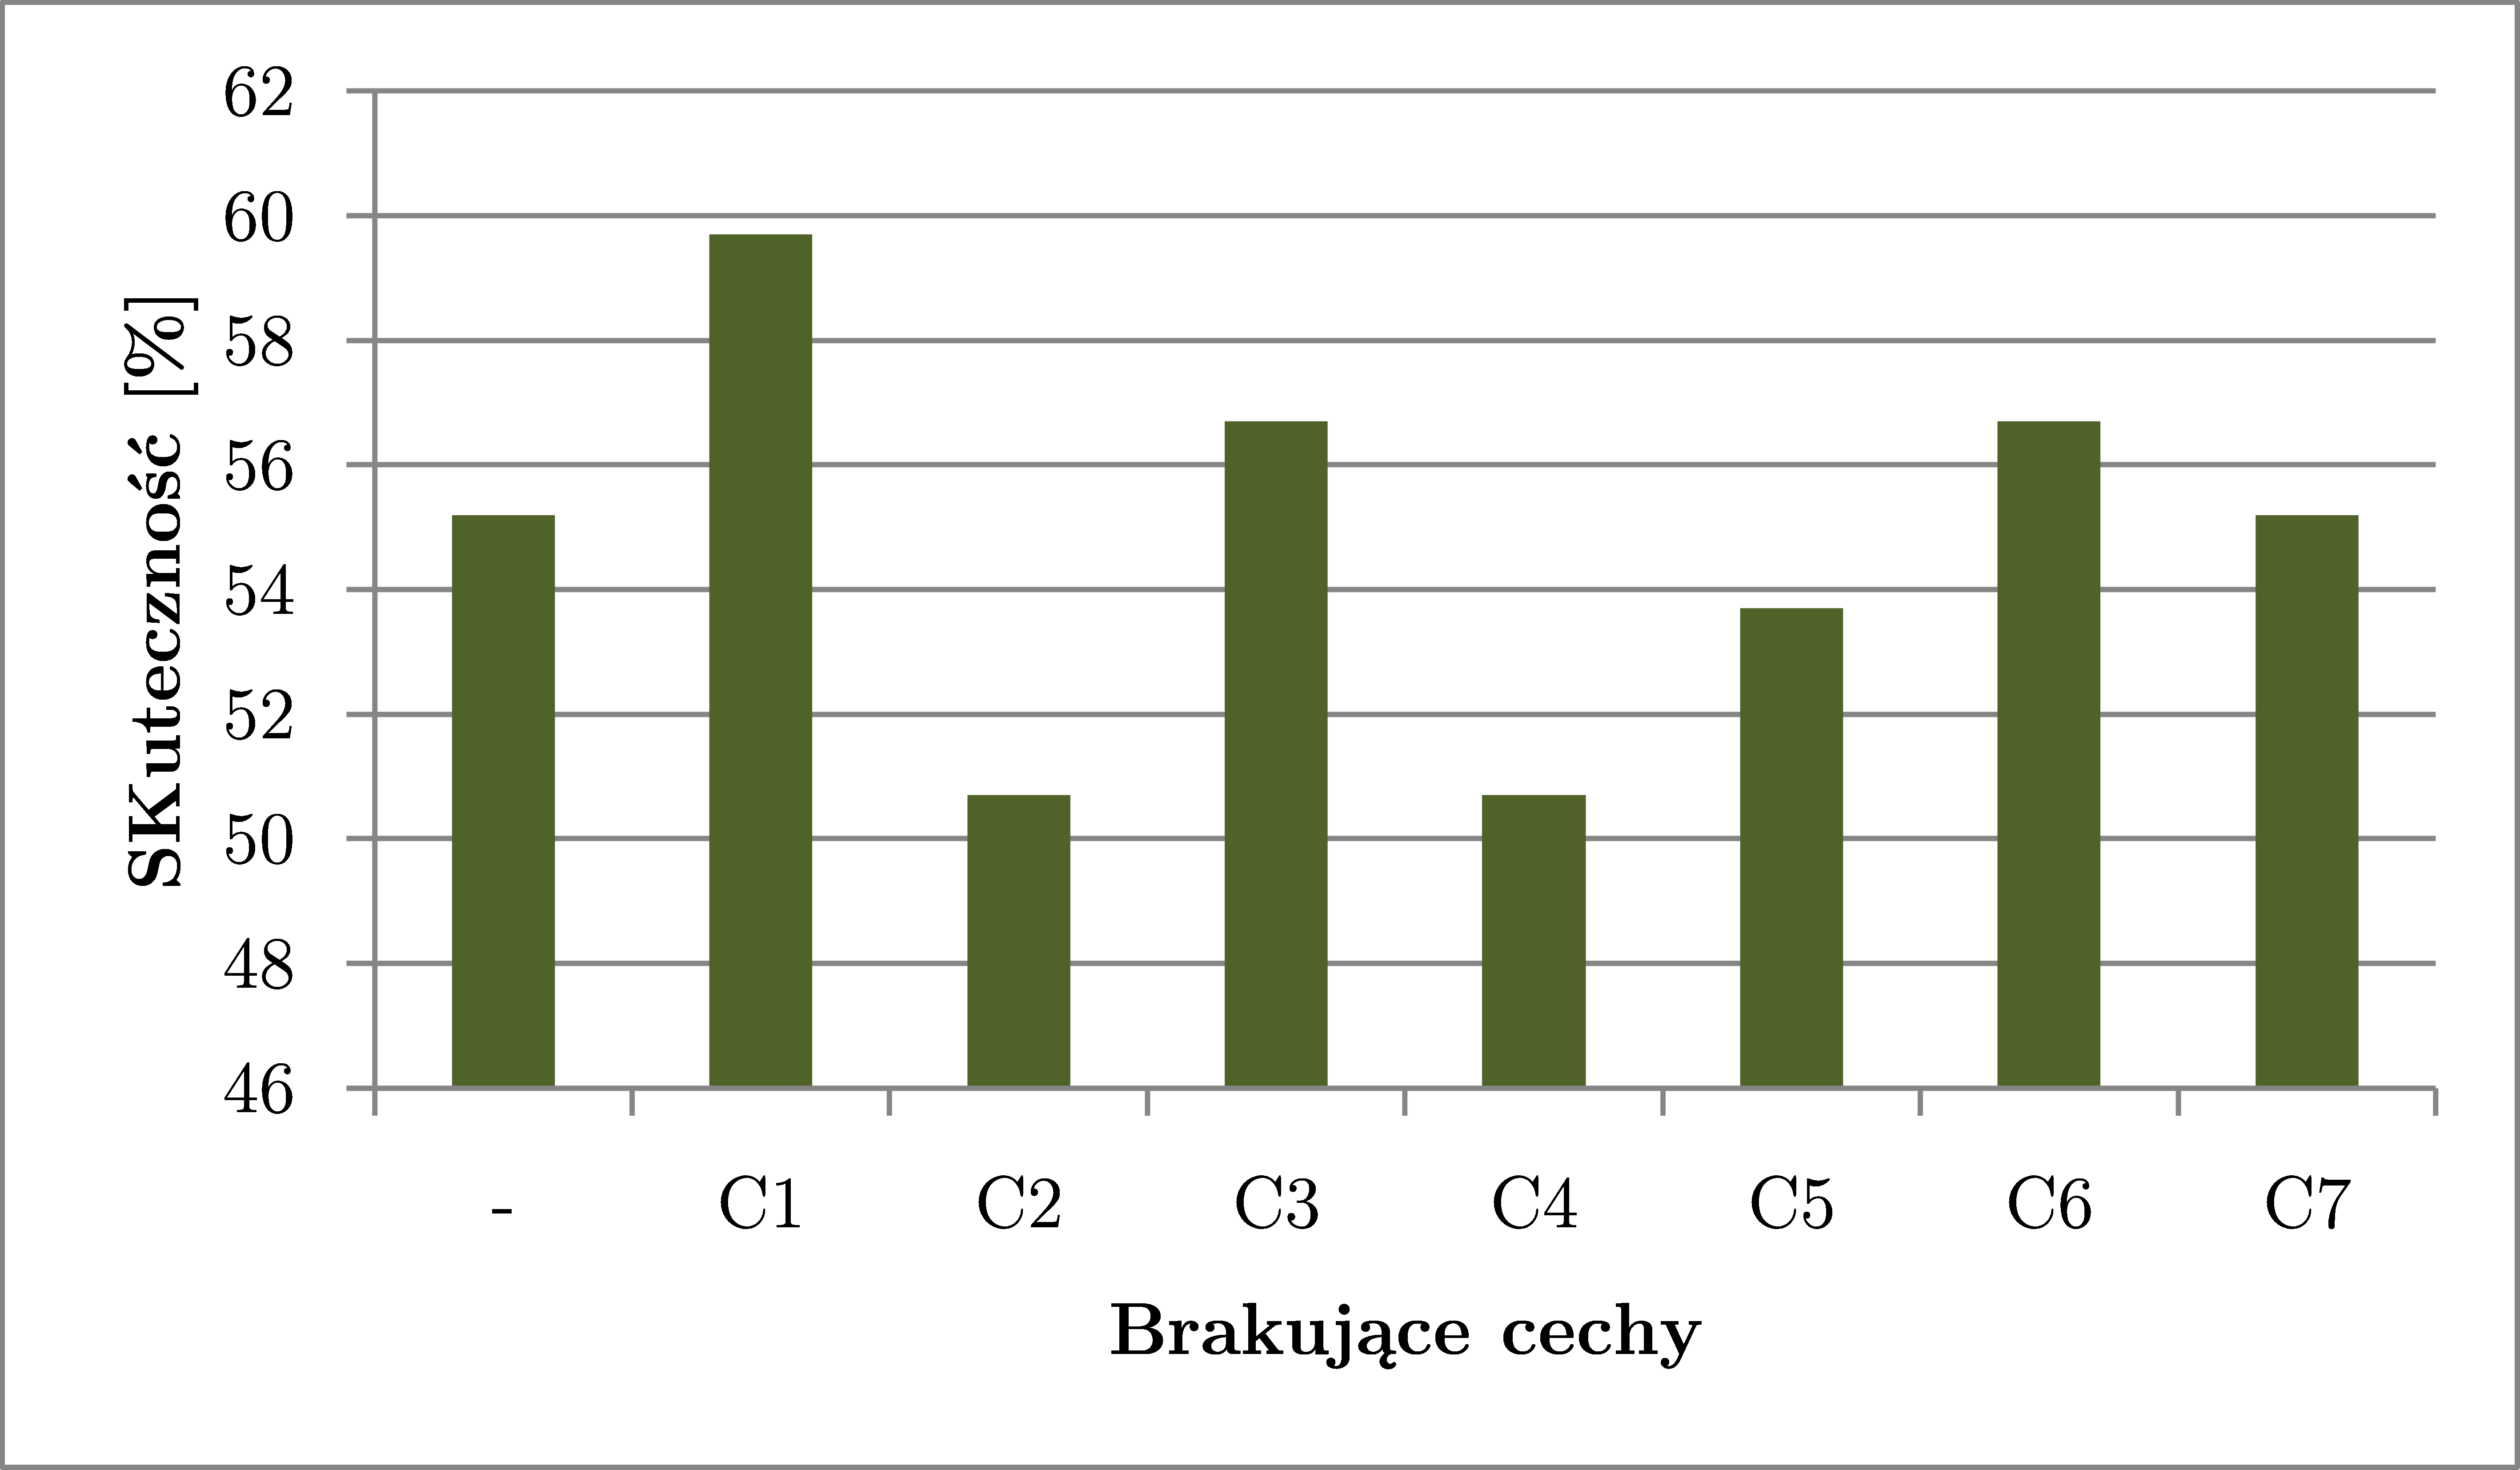
\includegraphics[width=0.9\textwidth]{{Rysunki/OWN-missing-topics.png}}
	\caption{Skuteczność klasyfikacji dla brakujących cech, dla kategorii topics}
\end{figure}

\begin{figure}[H]
	\centering
	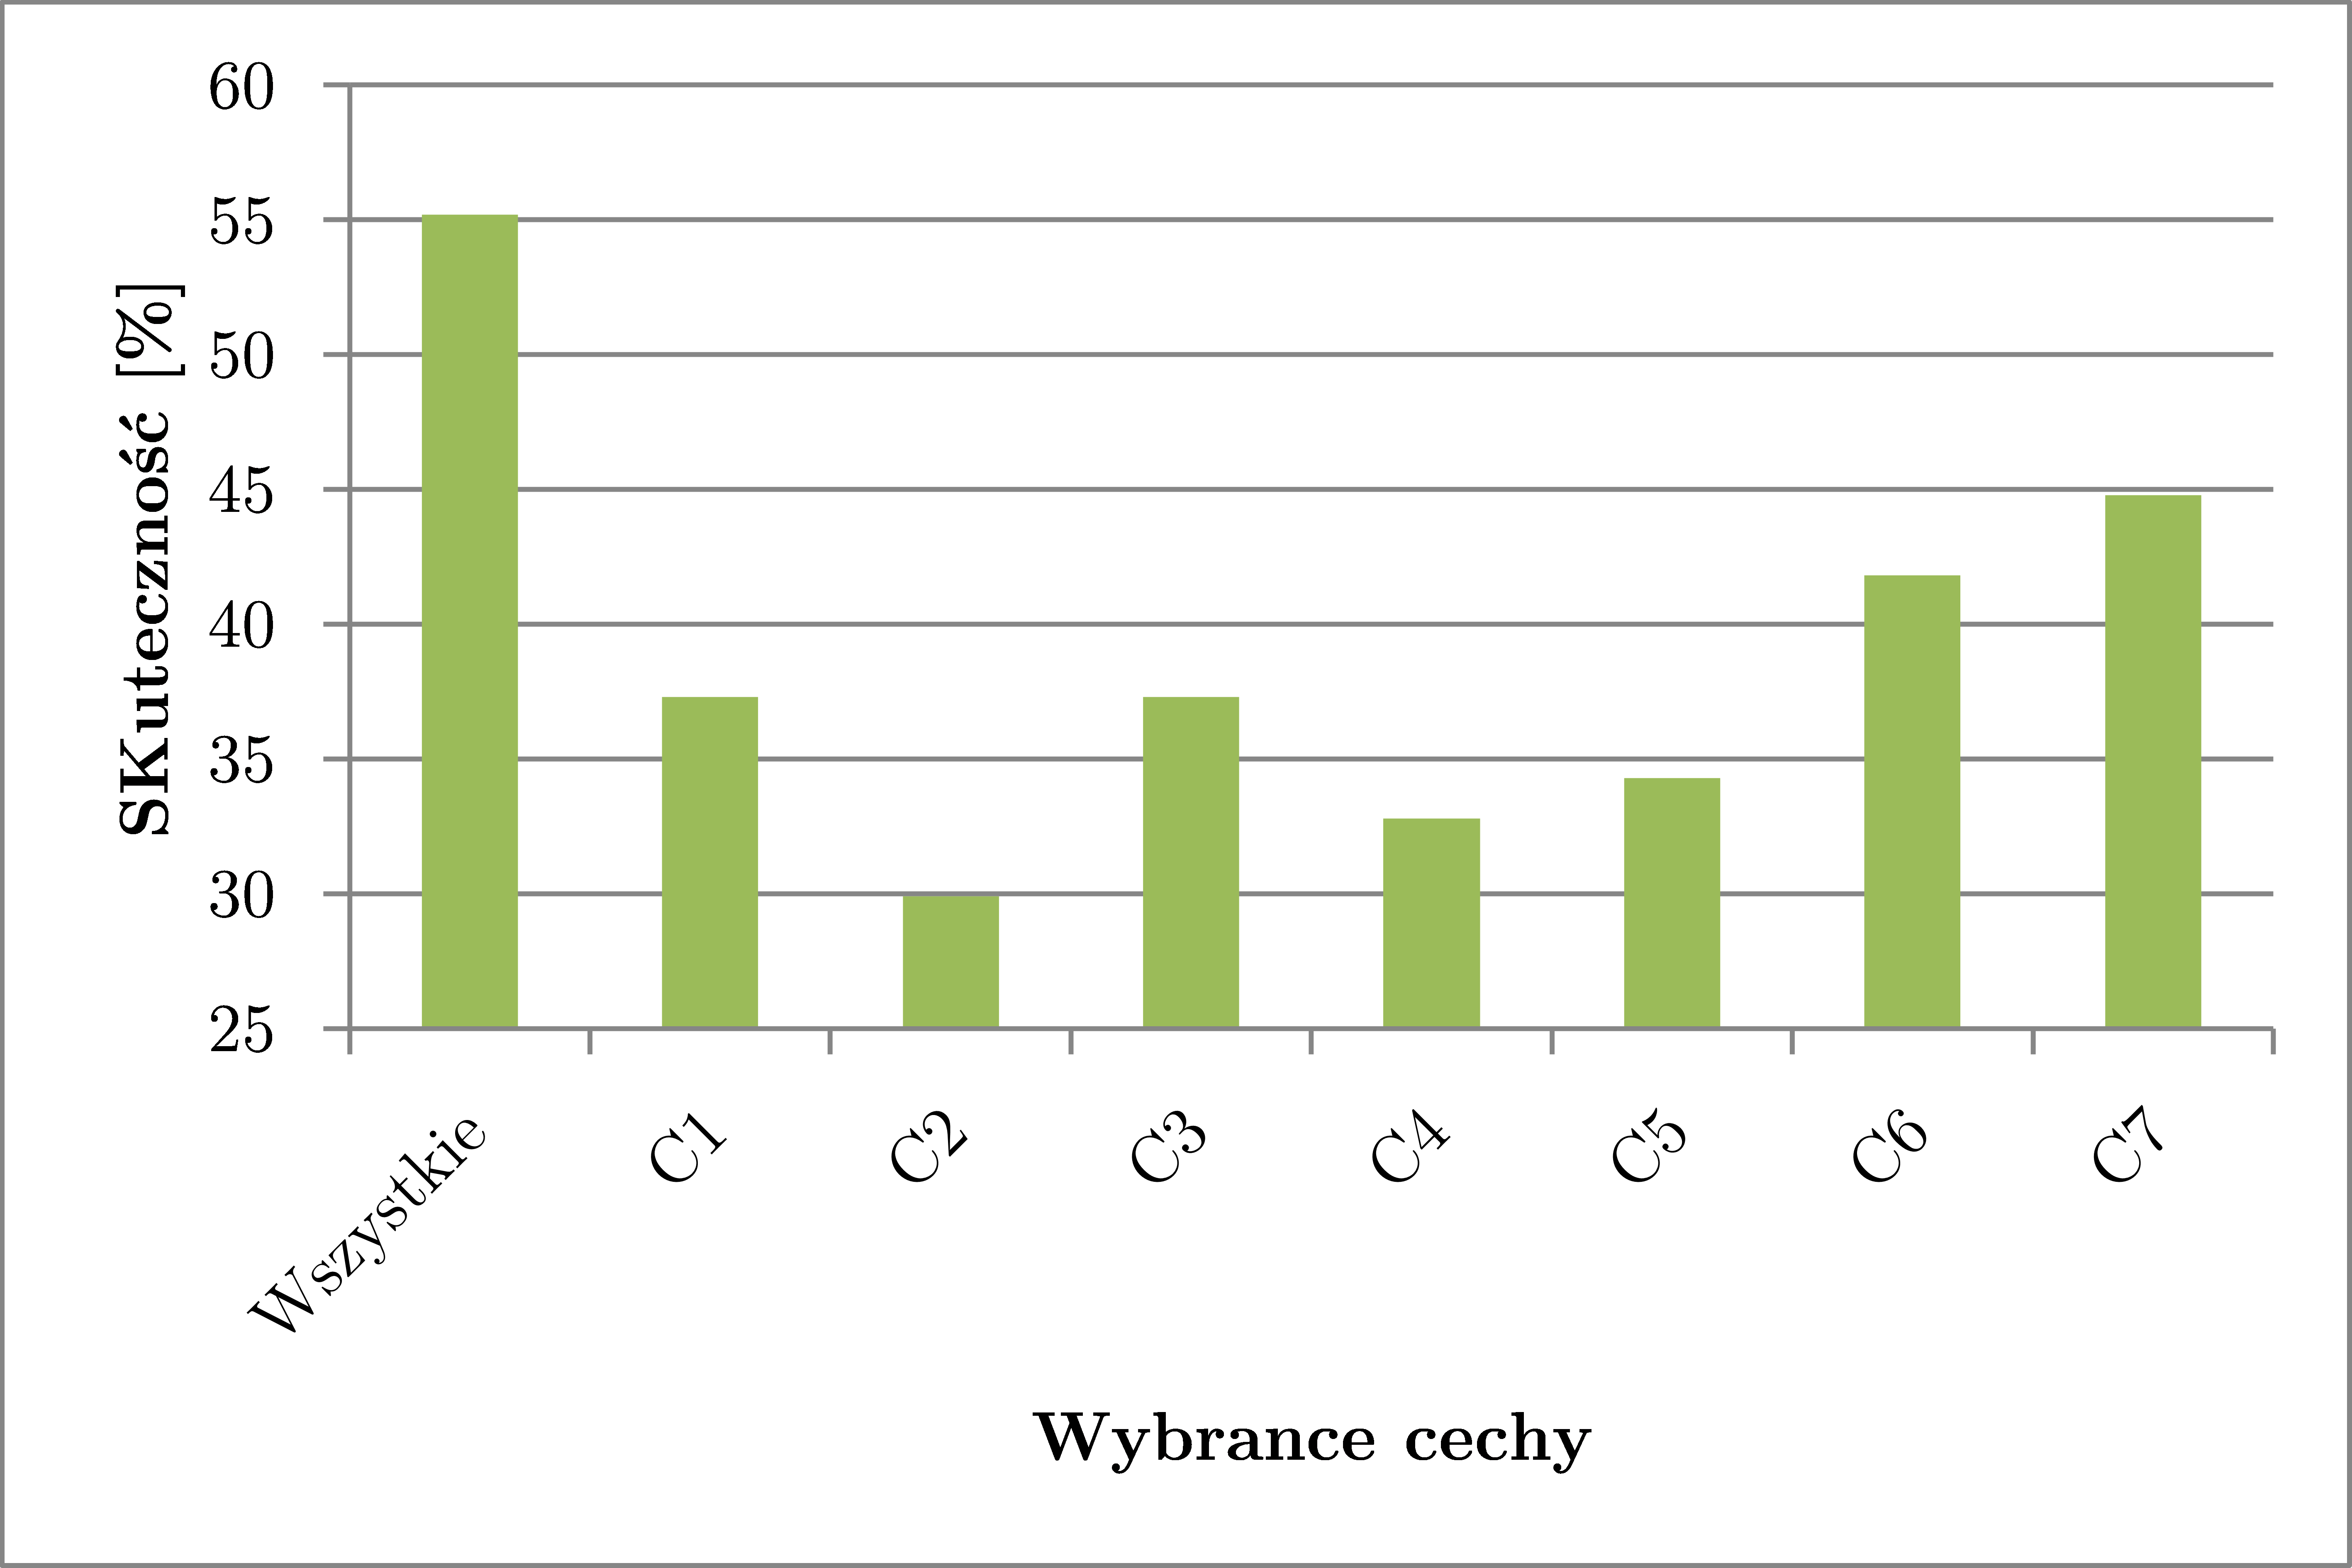
\includegraphics[width=0.9\textwidth]{{Rysunki/OWN-chosen-topics.png}}
	\caption{Skuteczność klasyfikacji dla wybranych cech, dla kategorii topics}
\end{figure}

\begin{figure}[H]
	\centering
	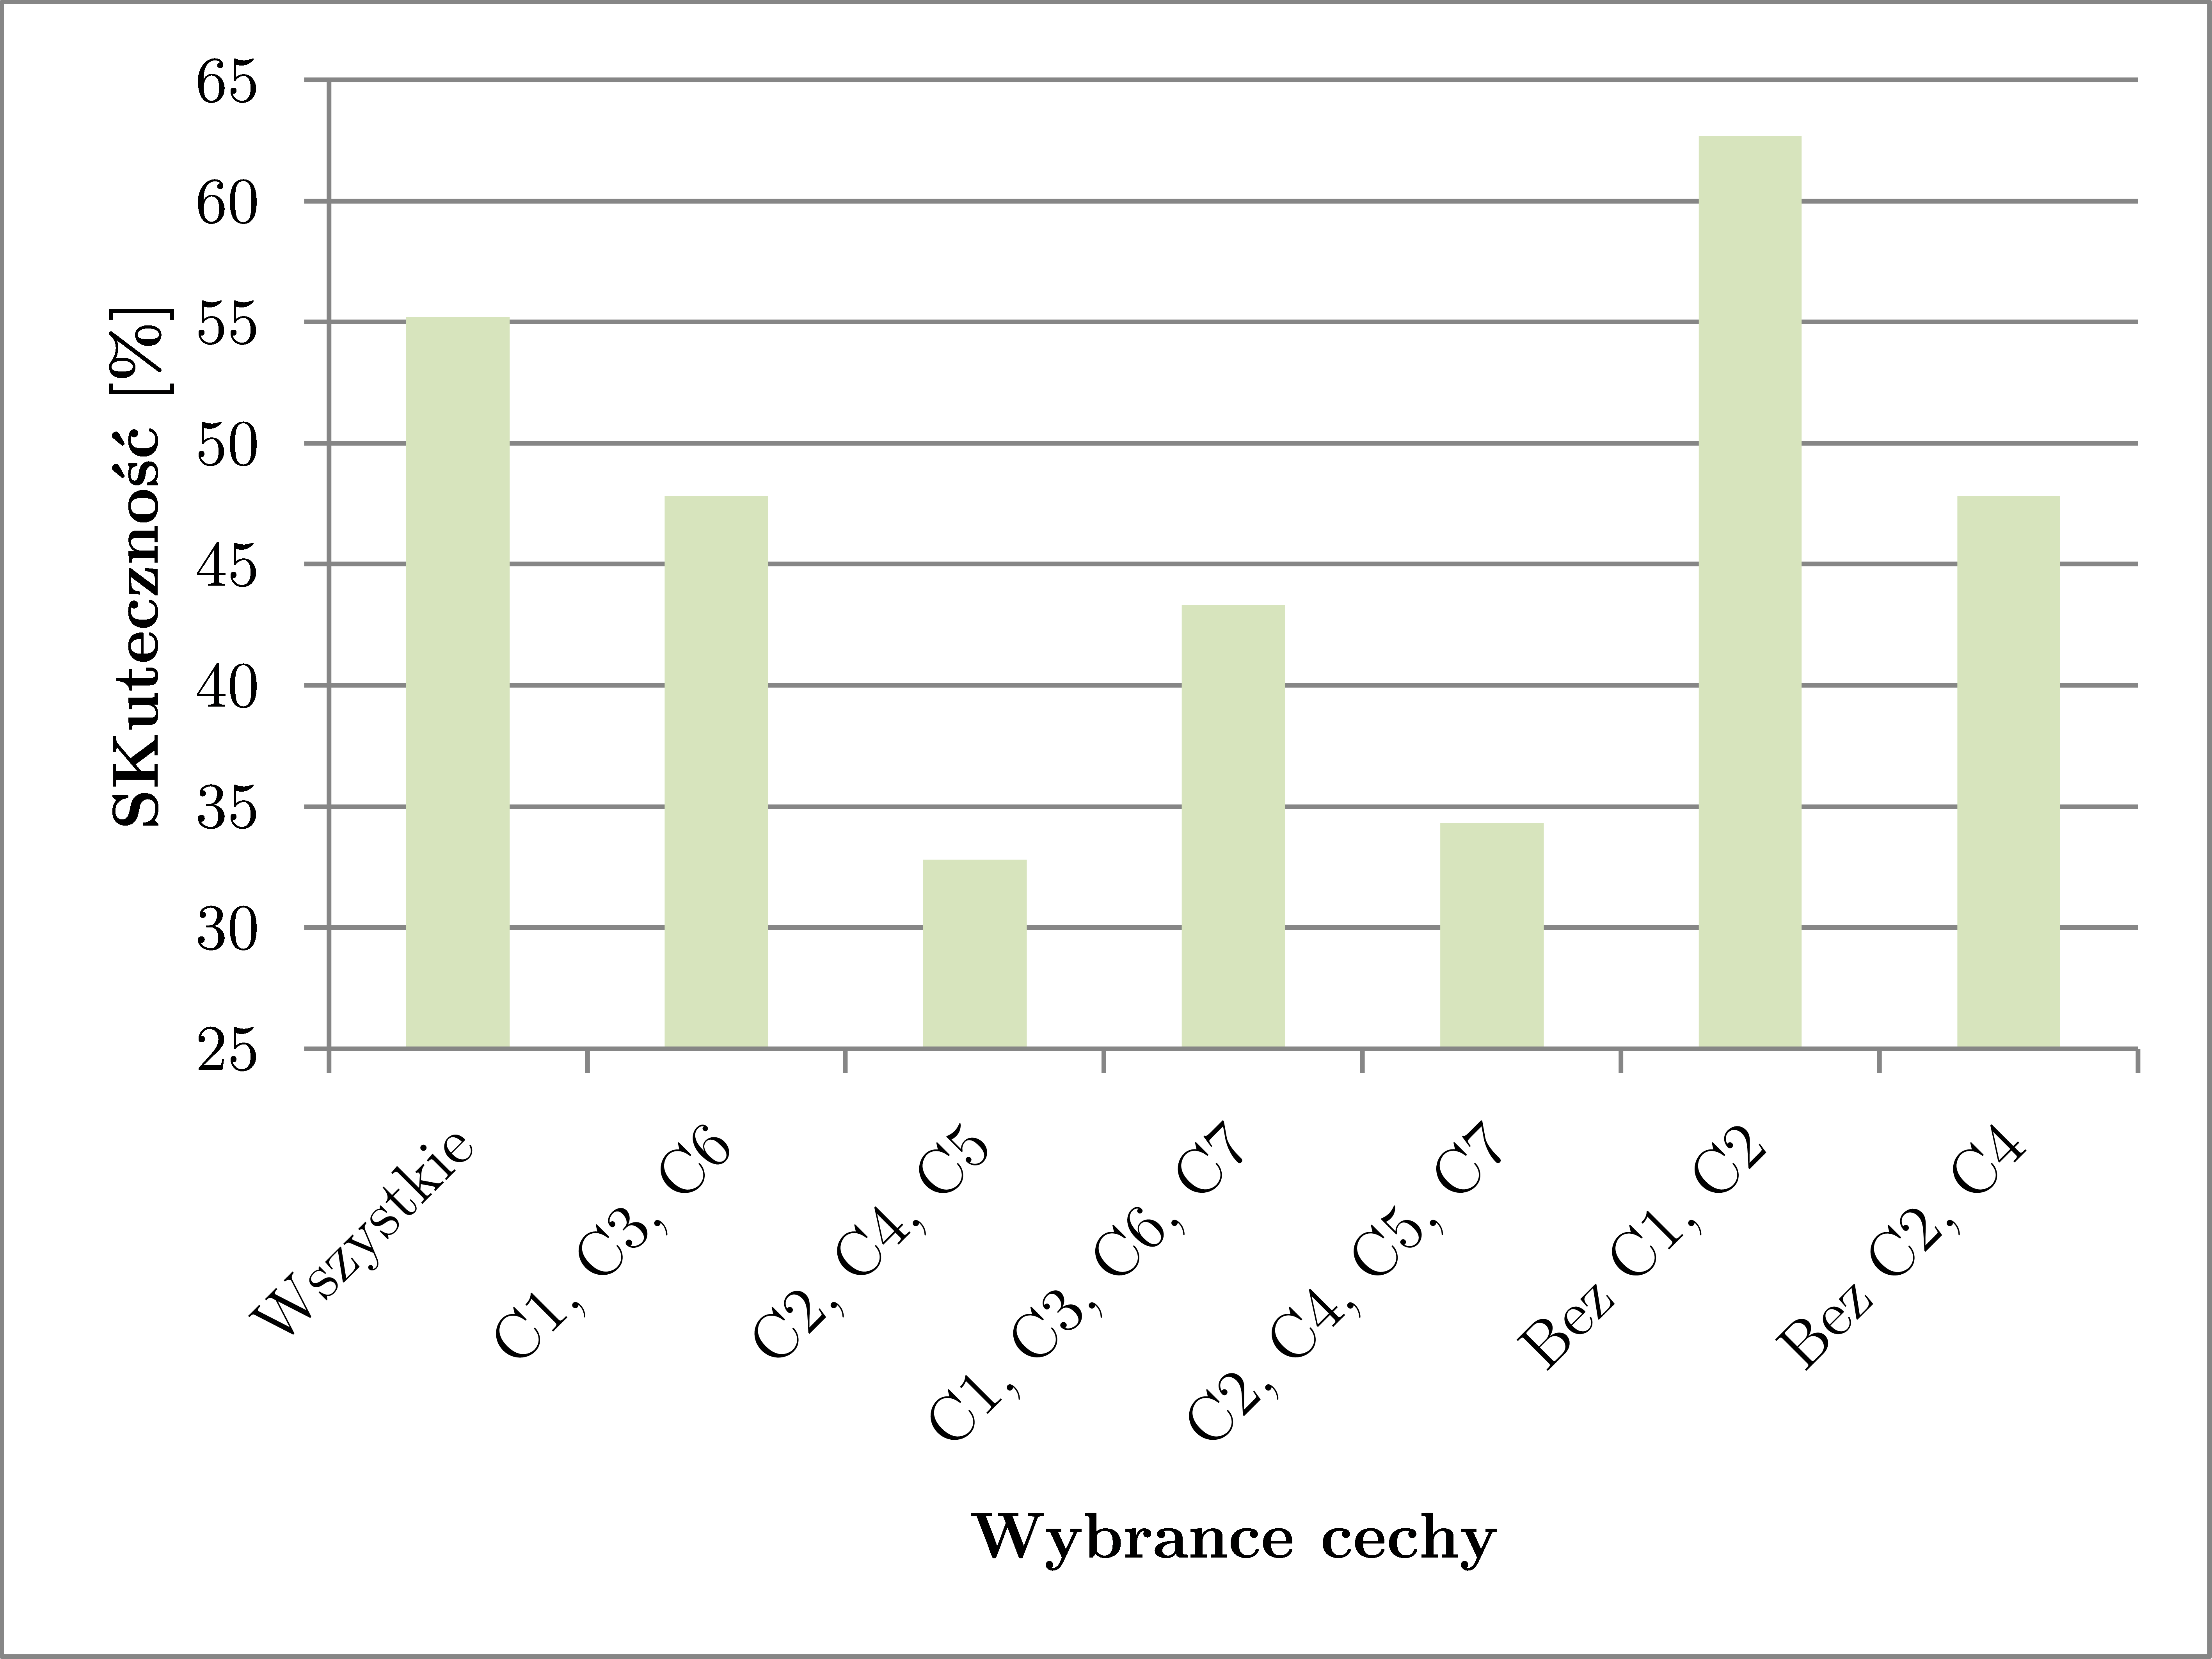
\includegraphics[width=0.9\textwidth]{{Rysunki/OWN-set-topics.png}}
	\caption{Skuteczność klasyfikacji dla zestawu cech, dla kategorii topics}
\end{figure}

\begin{figure}[H]
	\centering
	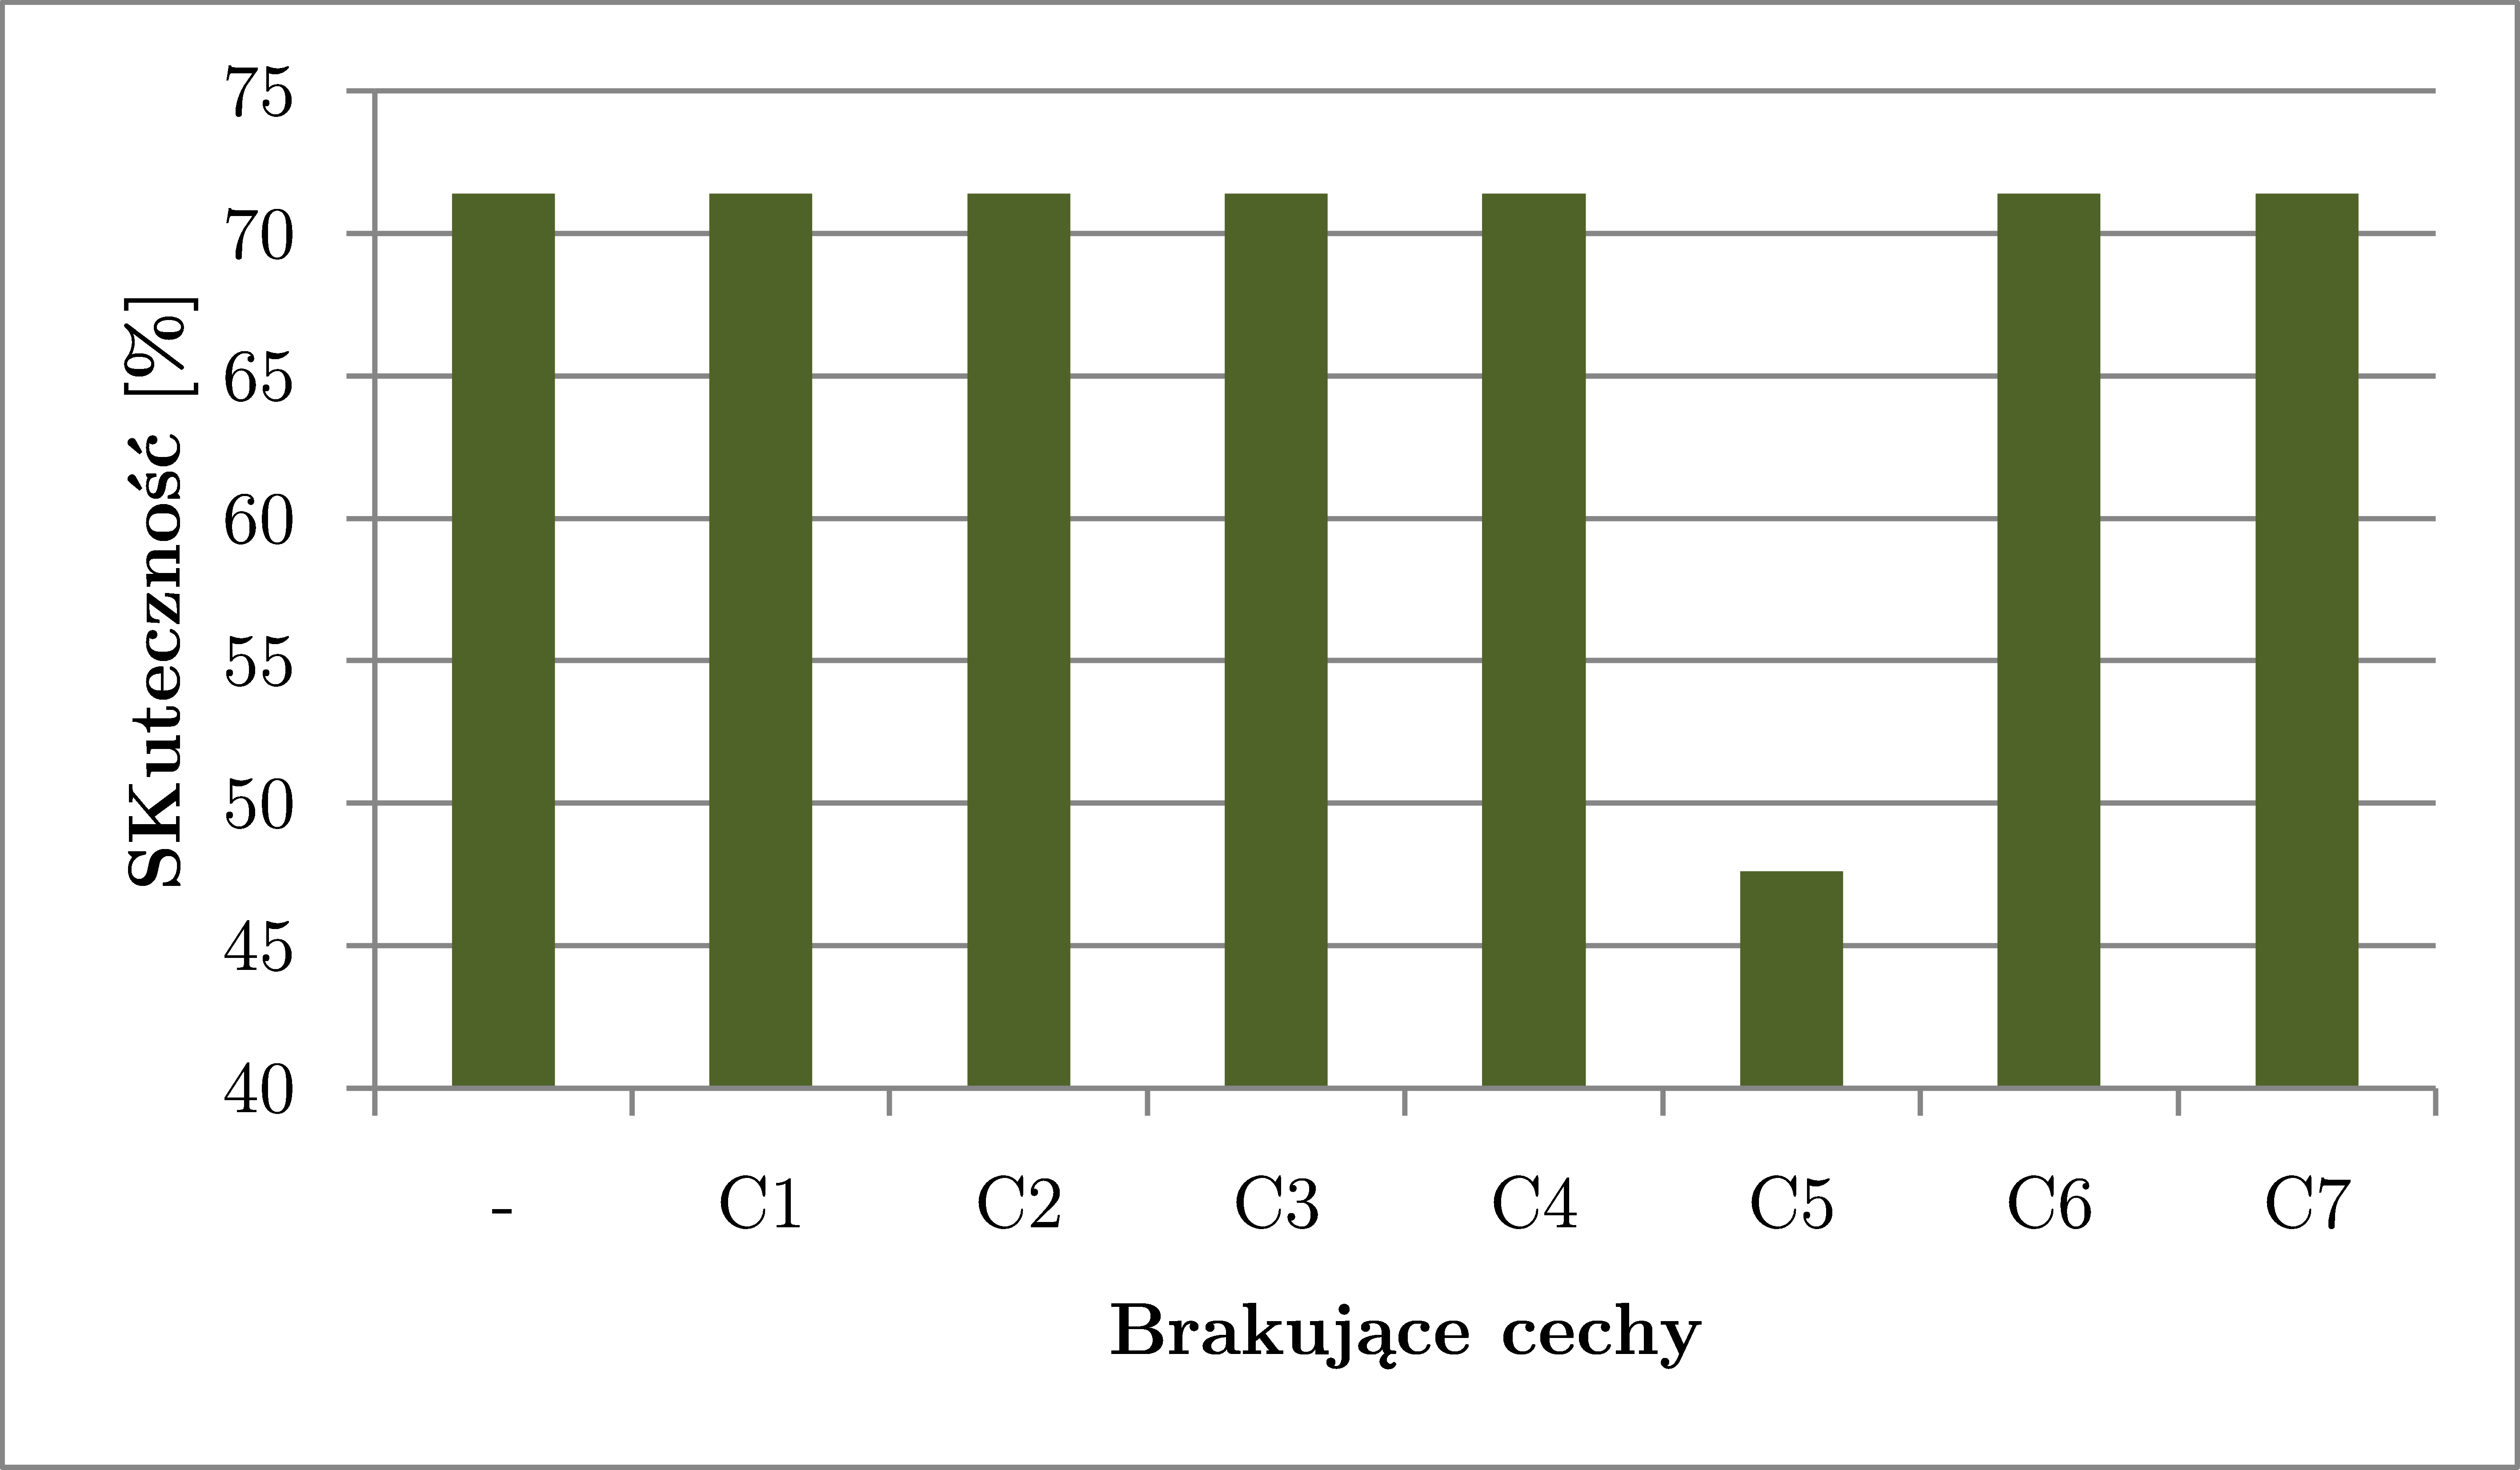
\includegraphics[width=0.9\textwidth]{{Rysunki/OWN-missing-authors.png}}
	\caption{Skuteczność klasyfikacji dla brakujących cech, dla kategorii authors}
\end{figure}

\begin{figure}[H]
	\centering
	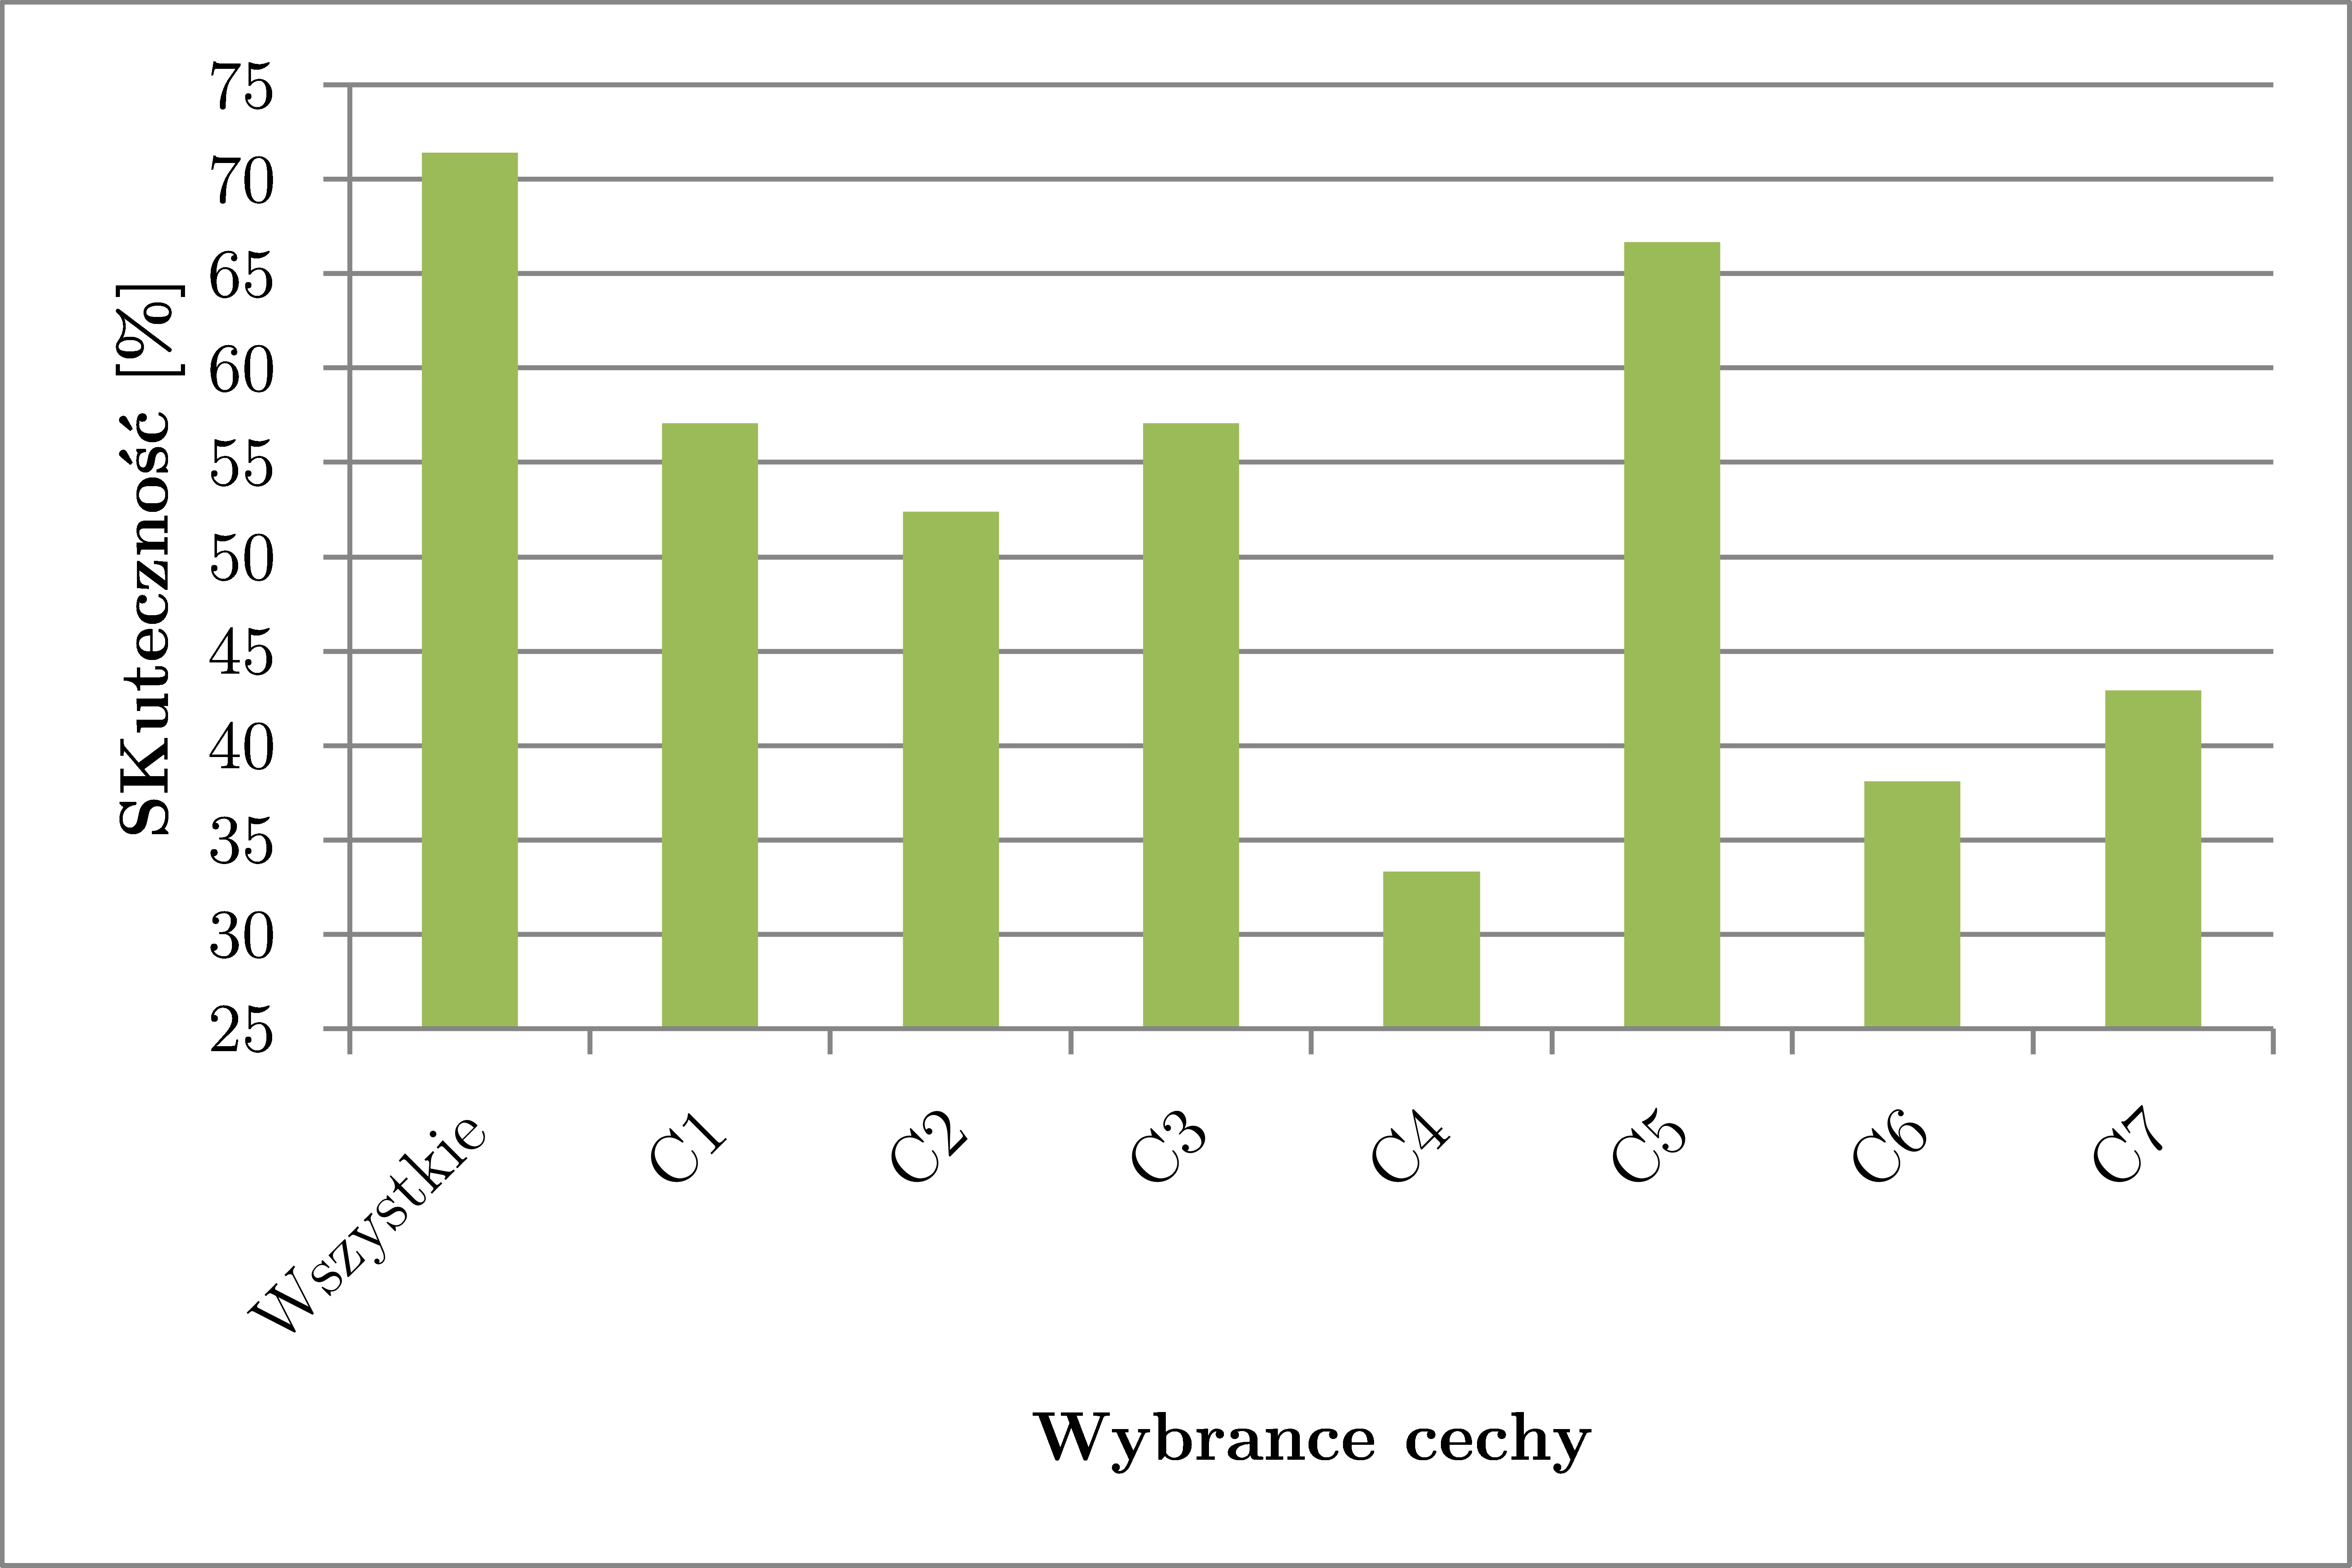
\includegraphics[width=0.9\textwidth]{{Rysunki/OWN-chosen-authors.png}}
	\caption{Skuteczność klasyfikacji dla wybranych cech, dla kategorii authors}
\end{figure}

\begin{figure}[H]
	\centering
	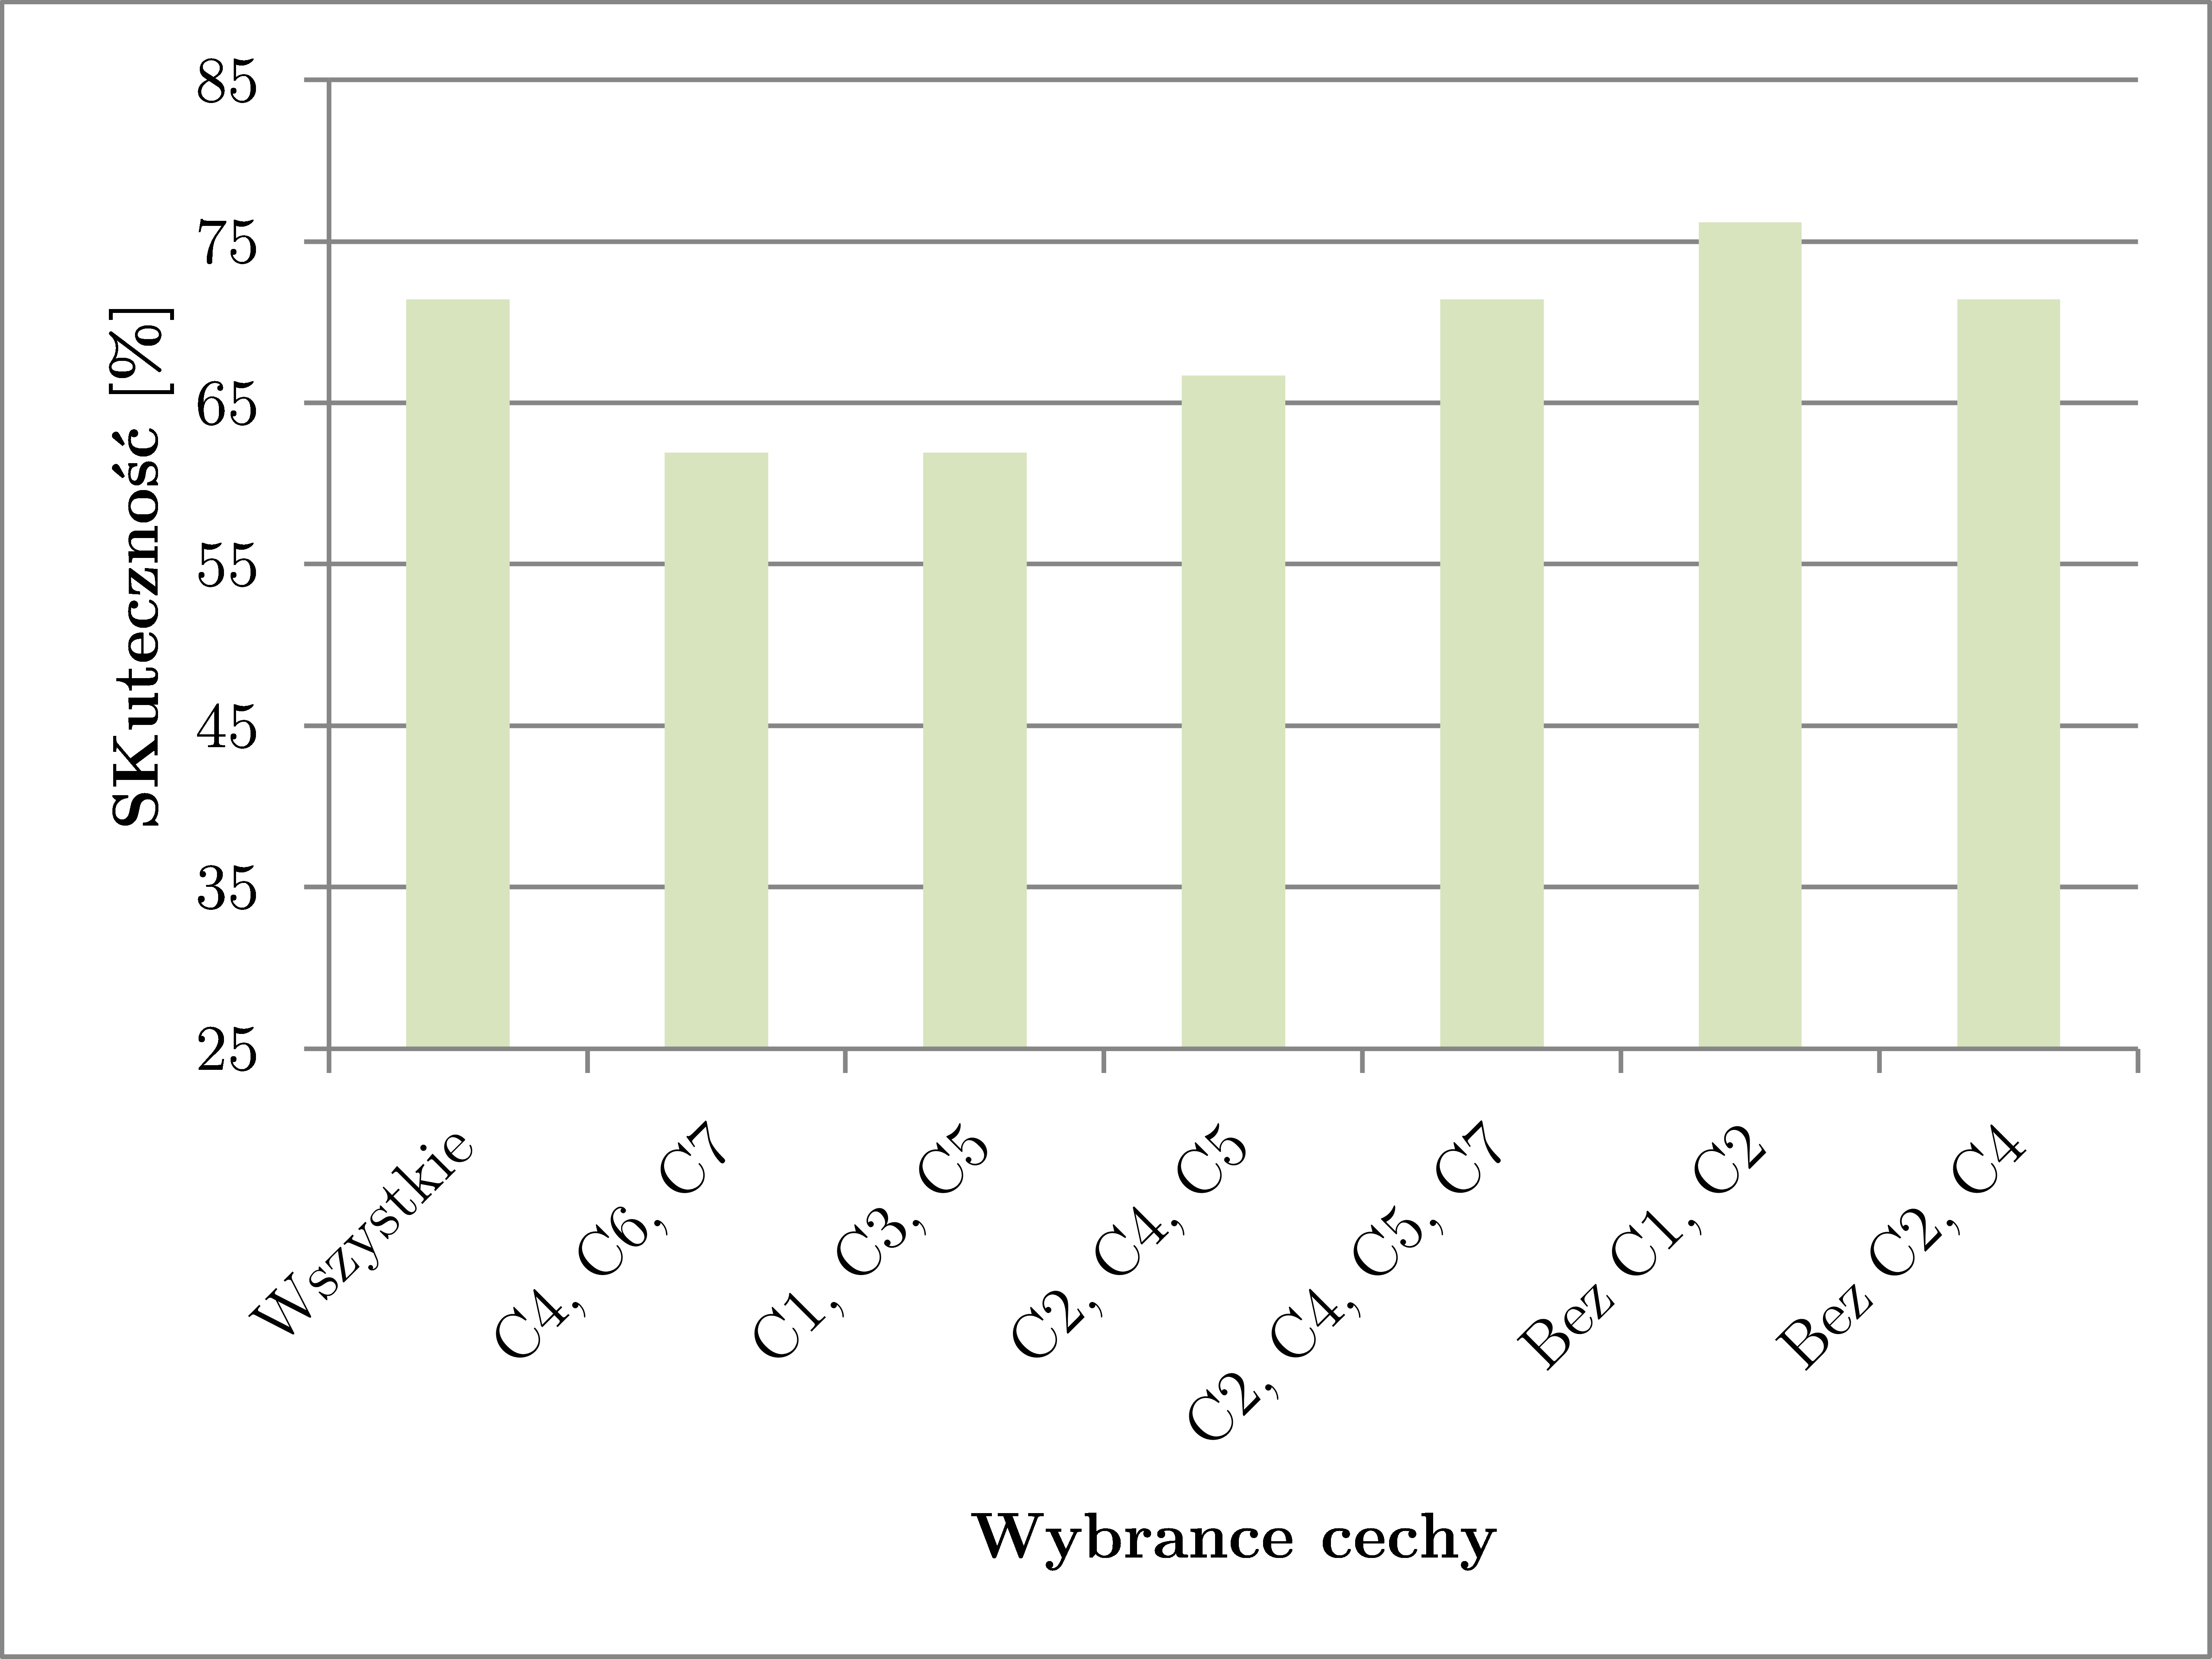
\includegraphics[width=0.9\textwidth]{{Rysunki/OWN-set-authors.png}}
	\caption{Skuteczność klasyfikacji dla zestawu cech, dla kategorii authors}
\end{figure}

\subsection{Najlepsze wyniki}
\begin{table}[H]
	\centering
	\begin{tabular}{c c c c c} 
		\hline
		\textbf{Kategoria} & \textbf{Skuteczność} & \textbf{Metryka} & \textbf{Ekstrakcja} &  \textbf{k} \\ [0.5ex]
		\hline
		\hline 
		Places & 83.3\% & Euklidesowa & IDF & 7 \\
		Places & 83.3\% & Uliczna & IDF & 7 \\
		Topics & 67.9\% & Euklidesowa & IDF & 15 \\
		Topics & 67.9\% & Uliczna & IDF & 20 \\
		Authors & 43.9\% & Euklidesowa & TF & 2, 3 \\
		\hline
	\end{tabular}
	\caption{Tabela przedstawiająca najlepsze wyniki z pierwszego eksperymentu (4.1)}
\end{table}

\begin{table}[H]
	\centering
	\begin{tabular}{c c c c c} 
		\hline
		\textbf{Kategoria} & \textbf{Skuteczność} & \textbf{Zb. treningowy} & \textbf{Ekstrakcja} &  \textbf{k} \\ [0.5ex]
		\hline
		\hline 
		Topics & 64.73\% & 40\% & TF & 15, 20 \\
		Authors & 43.9\% & 60\% & TF & 2, 3 \\
		Topics & 55.2\% & 80\% & Własne cechy & 3-10 \\
		Authors & 71.4\% & 80\% & Własne cechy & 7, 15, 20 \\
		\hline
	\end{tabular}
	\caption{Tabela przedstawiająca najlepsze wyniki z drugiego eksperymentu (4.2)}
\end{table}

\begin{table}[H]
	\centering
	\begin{tabular}{c c c} 
		\hline
		\textbf{Kategoria} & \textbf{Skuteczność} & \textbf{Wykorzystane cechy} \\ [0.5ex]
		\hline
		\hline 
		Topics & 62,7\% & $c_{3}$, $c_{4}$, $c_{5}$, $c_{6}$, $c_{7}$ \\
		Authors & 76,2\% & $c_{3}$, $c_{4}$, $c_{5}$, $c_{6}$, $c_{7}$ \\
		\hline
	\end{tabular}
	\caption{Tabela przedstawiająca najlepsze wyniki z trzeciego eksperymentu (4.3)}
\end{table}

\section{Dyskusja}

\subsection{Wpływ liczby k sąsiadów oraz wyboru metryki na klasyfikację}
W przypadku wszystkich trzech sposobów ekstrakcji, metryka Euklidesowa oraz metryka uliczna osiągają bardzo podobne wyniki i nie jesteśmy w stanie stwierdzić, która z nich wykazuje lepszą skuteczność. Metryka Czebyszewa charakteryzuje się zdecydowanie słabszą zdolnością do klasyfikacji. Osiąga niższe wyniki, niż dwie wcześniej wspomniane metryki.
 \newline

W przypadku pierwszego i drugiego sposobu ekstrakcji cech dla kategorii topics i places, zauważyliśmy, że wraz ze wzrostem liczby k sąsiadów zwiększała się także skuteczność. Najsłabsze wyniki osiągane były dla k równego 2. Jeśli zaś chodzi o kategorię authors, najwyższa skuteczność wykazywała mała liczba k sąsiadów (od 2 do 3). Wyraźny spadek wyników zaobserwowaliśmy, gdy k równało się 10. Podczas eksperymentu trzeciego sposobu ekstrakcji cech zauważyliśmy bardzo zmienną skuteczność w przypadku zmiany liczby k sąsiadów w zależności od wybranych kategorii. Kategoria places osiąga najsłabsze wyniki przy małej liczbie sąsiadów, z kolei kategoria topics najlepsze. Zauważyliśmy, że najwyższe wyniki w kategorii authors osiągane są przy liczbie sąsiadów równej 7 oraz 10. 


\subsection{Wpływ podziału tekstów na zbiory treningowe i testowe na klasyfikację}
W przeważającej większości najwyższe wyniki osiągane były przy 80\% zbioru treningowego. Tylko w jednym przypadku użycie 40\% zbioru treningowego pozwoliło osiągnąć najwyższą skuteczności (pierwszy sposób ekstrakcji, kategoria topics). Zazwyczaj jednak ten dobór procentowy okazywał się być najsłabszym ze względu na niedouczenie. 
\newline

\subsection{Wpływ konkretnych cech na klasyfikację}
Podczas klasyfikacji dla kategorii topics, zauważyliśmy, że liczba słów oraz liczba słów, których długość nie przekracza 3 znaków mają negatywny wpływ na osiąganą skuteczność. Świadczyć może o tym fakt, iż bez ww. cech osiągnęliśmy najwyższą skuteczność. Dużo ważniejsze okazały się cechy związane z unikalnością słów oraz wielkimi literami. \newline

Podczas klasyfikacji dla kategorii authors najważniejsza okazała się cecha odpowiadająca za liczbę unikalnych słów. Bez niej skuteczność spadła z 71\% na 47\%. Podobnie jak w przypadku kategorii topics, cechy sprawdzające liczbę słów oraz liczbę krótkich słów osłabiały nasze wyniki - dzięki wyłączeniu ich, uzyskaliśmy wyższe wyniki niż w przypadku wszystkich cech. 

	
\section{Wnioski}
\begin{itemize}
	\item Liczba k sąsiadów ma spory wpływ na skuteczność klasyfikacji, jednak nie ma jednej, optymalnej wartości - zmiana metryki, podziału zbiorów czy klasyfikowanych kategorii może spowodować obniżenie wyników dla stałego k.
	\item Dla mniejszych zbiorów tekstowych lepiej sprawdzają się mniejsze wartości k sąsiadów, dla większych - wyższe wartości.
	\item Metryka Czebyszewa nie powinna być wykorzystywana w klasyfikacji tekstów, gdyż osiąga bardzo słabe wyniki.
	\item Istotny jest podział tekstów na zbiory testowe oraz treningowe. W przypadku zbyt małego zbioru treningowego osiągamy zjawisko niedouczenia, w przypadku zbyt dużego - przeuczenia.
	\item Cechy odpowiedzialne za liczbę słów oraz liczbę krótkich słów (do 3 znaków)  nie sprawdzają się przy klasyfikacji tekstów.
	\item Wektor cech powinien się składać z przynajmniej kilku cech, żeby osiągnąć większą skuteczność.
\end{itemize}

	

\begin{thebibliography}{}
\bibitem{adam}
Methods for the linguistic summarization of data - aplications of fuzzy sets and their extensions, Adam Niewiadomski, Akademicka Oficyna Wydawnicza EXIT, Warszawa 2008
\bibitem{AGH}
http://home.agh.edu.pl/~horzyk/lectures/miw/KNN.pdf
\bibitem{Stop Lista}
https://github.com/hklemp/dotnet-stop-words
\bibitem{Stemizacja}
http://snowball.tartarus.org/algorithms/english/stemmer.html
\end{thebibliography}
\end{document}
